% MH6805 Machine Learning in Finance --- Group Project Final Report, Group B19
% Typeset with the NeurIPS 2021 style file supplied by the instructor.
% Build:  ./build_report_tex.sh      (body must stay within 7 pages INCLUDING references;
%                                     the appendix is exempt under the course guideline)
\documentclass{article}

% [preprint] is the option the template prescribes for a non-anonymous paper that is not a
% NeurIPS acceptance: it typesets the real \author block (the contribution statement is
% mandatory for this course) and does not load the anonymous-submission line numbers.
% [final] is deliberately NOT used --- the template reserves it for accepted papers.
\usepackage[preprint]{neurips_2021}

\usepackage[utf8]{inputenc}
\usepackage[T1]{fontenc}
\renewcommand{\ttdefault}{lmtt}      % Type 1 T1 typewriter: no bitmap fonts in the PDF
\usepackage{xcolor}                  % red draft percentages in the contribution statement
\usepackage[hidelinks]{hyperref}
\usepackage{url}
\usepackage{booktabs}
\usepackage{amsfonts}
\usepackage{graphicx}
\usepackage{array}
\usepackage{longtable}
\graphicspath{{../figures/}}

% Unicode characters that appear in the drafted text.
\DeclareUnicodeCharacter{2212}{\ensuremath{-}}
\DeclareUnicodeCharacter{2265}{\ensuremath{\ge}}
\DeclareUnicodeCharacter{2264}{\ensuremath{\le}}
\DeclareUnicodeCharacter{2248}{\ensuremath{\approx}}
\DeclareUnicodeCharacter{00D7}{\ensuremath{\times}}
\DeclareUnicodeCharacter{2192}{\ensuremath{\rightarrow}}
\DeclareUnicodeCharacter{2026}{\dots}
\DeclareUnicodeCharacter{00B1}{\ensuremath{\pm}}
\DeclareUnicodeCharacter{2013}{--}
\DeclareUnicodeCharacter{2014}{---}

% The style file prints a venue line at the foot of page 1. This is coursework, so the slot
% carries the course identification instead of "Preprint. Under review."
\makeatletter
\renewcommand{\@noticestring}{%
  MH6805 Machine Learning in Finance, Nanyang Technological University.
  Group project final report, Group B19.}
\makeatother

\newcolumntype{L}[1]{>{\raggedright\arraybackslash}p{#1}}

\title{Predicting Credit-Card Default:\\ A Comparative Study of\\ Machine-Learning Classifiers}

\author{%
  RUAN Hangjing\\
  G2607546F\\
  \texttt{hangjing001@e.ntu.edu.sg}
  \And
  LU Xinyu\\
  G2603537D\\
  \texttt{xinyu057@e.ntu.edu.sg}
  \And
  LI Jingwen\\
  G2607526K\\
  \texttt{jingwen013@e.ntu.edu.sg}
}

\begin{document}
\maketitle

\begin{abstract}
  Because a missed defaulter costs several times a false alarm, a default model
  must be judged at an operating point, not by ranking alone. We compare ten
  classifiers on the UCI credit-card default data (29,965 Taiwanese card holders,
  22.1\% defaulters) against a $K$-nearest-neighbour benchmark and a logistic
  baseline, every choice made on training rows and each configuration scored
  once on a frozen 30\% test set. Tree ensembles rank best (XGBoost: test
  AUC 0.789, average precision 0.578) but gain only 0.025 AUC over the logit, the
  random forest is indistinguishable from XGBoost, and six months of repayment
  status carry nearly all the signal, additively. Class weights, SMOTE and
  under-sampling inside the folds move the intercept, not the ranking. At a 5:1
  cost ratio, moving the logit's cut-off from 0.5 to 0.15 saves 1,937 [1,604,
  2,218] of its 7,063 test cost units; switching to XGBoost saves a further 145
  [$-$18, 299].
\end{abstract}

\paragraph{Contribution statement.}
Group B19. Model families are owned end to end (code, tuning, interpretation,
presentation): RUAN Hangjing the KNN benchmark, the logistic family, nested
cross-validation and PCA/K-means; LU Xinyu the pruned tree, random forest and
bagging, gradient boosting and XGBoost, TreeSHAP, monotone constraints and
partial dependence; LI Jingwen the support-vector machines, the neural network,
LDA/QDA/naive Bayes, the class-imbalance study and leakage demonstration, Platt
recalibration, and the freeze and aggregation code. Shares per section (RUAN/LU/LI, \%):
\S1~\textcolor{red}{30/20/50}; \S2~\textcolor{red}{25/15/60};
\S3~\textcolor{red}{30/25/45}; \S4~\textcolor{red}{30/35/35};
\S5~\textcolor{red}{15/60/25}; \S6~\textcolor{red}{40/15/45};
\S7~\textcolor{red}{34/33/33}; code and reproducibility
\textcolor{red}{20/25/55}; presentation \textcolor{red}{33/33/34}
(Table~\ref{tab:a-workload}; red = draft awaiting the group's confirmation). Not shared with any other module.

\section{Introduction}

Unsecured revolving credit is one of the largest sources of loss for a retail
bank: a defaulter's balance is written off, while the upside on a good customer
is a thin monthly margin. The two errors are not symmetric, so a model that merely ranks clients
well is not yet a decision; the question is which model, at which cut-off.

The study is comparative in the sense of the course [6] rather than a hunt for
a winner. Two models are the reference points --- a $K$-nearest-neighbour
classifier, the non-parametric benchmark, and a logistic regression, the
scorecard a credit department could defend to a regulator --- and every other
family is read against them, each gap explained by a mechanism rather than a
rank. Ranking is judged by ROC-AUC and average precision, calibration by the
Brier score and the decision by expected cost; accuracy is context only. Three
methods beyond the syllabus --- TreeSHAP [7], a monotonically constrained
XGBoost and partial dependence [4] --- carry the inference. Four questions
organise what follows. (1)~\emph{Value of complexity}: how much ranking quality do
non-linear and ensemble methods add over the two reference models, beyond
test-set noise? (2)~\emph{Operating point}: cut at 0.5, at maximum $F_1$, or at
the threshold implied by an asymmetric cost --- and does that choice outweigh the
model's? (3)~\emph{Class imbalance}: do class weights, SMOTE and under-sampling
inside the folds help, and what does resampling before the split fabricate?
(4)~\emph{Inference}: which characteristics drive default, in which direction, and
do the coefficient, impurity, permutation and Shapley accounts agree?
          % abstract, contribution statement, introduction, objectives
\section{Data}

\paragraph{Source, scope and what the label means.}
The data are 30,000 existing cardholders of one Taiwanese bank (\emph{Default of Credit Card Clients}, UCI Machine Learning Repository, \url{https://archive.ics.uci.edu/dataset/350/default+of+credit+card+clients}, doi:10.24432/C55S3H, CC~BY~4.0 [18]; described in [19]). We predict default on the October 2005 payment from April--September 2005 histories, so a flag triggers an account-management action on a current client (a call, a reminder, a limit review), not an approval. The monthly variables precede the label; the limit and demographics are undated snapshots, assumed recorded by September 2005 (if the bank cut limits after missed payments, the limit would partly record the outcome). Removing 35 rows that repeat another client's record exactly, label included (mostly dormant profiles), leaves 29,965 clients, 29 predictors (Table~\ref{tab:a-variables}) and 22.1\% defaulters: ``never default'' is 77.9\% accurate yet catches nobody. Code: \href{https://github.com/jingwen013-design/mh6805-credit-default}{\texttt{github.com/jingwen013-design/mh6805-credit-default}} (\texttt{code/run\_all.sh} regenerates every number).

\paragraph{Repayment codes are states, not a scale.}
PAY\_1--PAY\_6 record each month's status: $-2$ no consumption, $-1$ paid in full, 0 revolving credit, $k \ge 1$ = $k$ months late (UCI documents only $-1$ and 1--9; the readings of $-2$ and 0 are widely used, not documented). Non-delinquent codes have no order: September default is 13.7\% at $-2$, 16.9\% at $-1$ and 12.9\% at 0 (training rows). Code 1 also changes meaning: it appears 2,540 times in September but 21 times in the five earlier months, mixing dormant accounts with clients recovering from two months late (Table~\ref{tab:a-paycodes-rates}), so compare codes within a month. A scorecard should weight these states separately (\S4).

\paragraph{Where the risk gradients are.}
Default rates change steeply with recent arrears and the limit, not with bill size. September default climbs from 12.9\% at revolving credit to 67.6\% at two months late, two payments already missed (code 1 is the mixture above). It falls steadily as the limit rises, but the bank sets the limit: a high limit marks a client it already judged safe, so raising a limit would not make anyone safer. Bill size alone ranks no better than chance (univariate area under the ROC curve, AUC, 0.50--0.52). Utilisation (bill over limit) is U-shaped: default is lowest for light users and highest near the limit, where no buffer is left. It is also above average with no positive balance, but most such clients carry the odd September code 1, so that arm is of uncertain meaning. Sex and age move the rate by at most 8 points (training rows; Table~\ref{tab:a-gradients}, Figures~\ref{fig:eda-default-rate-by-pay1}--\ref{fig:eda-default-rate-util-delay}).

\paragraph{What happens before the split.}
Three fixed steps estimate nothing, so they precede the split; everything estimated (scaling, one-hot levels, resampling, thresholds) is re-fitted inside each fold's \texttt{Pipeline} (Table~\ref{tab:a-quality}). (i)~An a-priori mapping of EDUCATION and MARRIAGE codes the UCI dictionary does not list (\{0,5,6\} and 0 to ``others''), so the ``others'' education bucket (343 training clients, 6.7\% default) is a coding artefact. (ii)~Six engineered features: two utilisation ratios, a payment ratio capped at 5, months in arrears, worst delay and balance trend (the delay counters count $-2$, $-1$ and 0 as 0). (iii)~Removal of the 35 repeated rows. Filling the payment ratio with 0 when all six bills are non-positive makes owing nothing look like paying nothing. The fill is not neutral: these 633 training clients default at 37.0\% against 21.7\%, so a bank must document it.
           % data, pre-split argument, exploratory findings
\section{Methods}

\paragraph{Protocol.}
The cleaned sample is split once, stratified on the target, into 20{,}975 training and 8{,}990 test clients under seed 2607526. Every choice --- hyper-parameters, thresholds, the CV winner and the top four --- is made on training rows (5-fold stratified cross-validation). Each configuration was frozen at its first test scoring: round 1, 34 variants by 18 September, before the professor's 30 September comment; RUAN Hangjing's second pass of 30 September, which re-fitted and re-scored two already-frozen configurations (KNN, plain logit) under her freeze-before-test protocol; the nine Platt-recalibrated versions on 19 October; plus the SMOTE-before-split negative control. The 46 entries are in \texttt{results/frozen\_manifest.json} (Table~\ref{tab:a-freeze}), and \texttt{common.evaluate()} refuses to re-score a changed configuration. The bootstrap and cost curves read the test rows but select nothing. Gradient boosting, bagging and the monotone XGBoost are not in the proposal's method table; their configurations were fixed a priori and each was scored once in round 1 (16--18 September). TreeSHAP, partial dependence and the drop-column refits are diagnostics of the fitted models on training rows only (Tables~\ref{tab:a-importance}--\ref{tab:a-refit}, Figure~\ref{fig:pdp-main}); they never read the test set. The three beyond the syllabus are the rows below the rule in Table~\ref{tab:a-methods}.

\paragraph{Preprocessing and metrics.}
Preprocessing is part of the model: standardisation, one-hot encoding of the three categorical columns and, in the imbalance study, resampling sit inside a scikit-learn \texttt{Pipeline} and are re-fitted on the training part of every fold. Tree models are fitted unscaled. Tuning grids, software versions and the monotone constraint vector are Tables~\ref{tab:a-tuning}--\ref{tab:a-monotone}. Two metrics, deliberately different: hyper-parameters are chosen by cross-validated ROC-AUC, because at tuning time the operating point is unknown, and the cut-off is a later decision on training out-of-fold probabilities (maximum $F_1$, or minimum expected cost at an assumed 5:1 false-negative to false-positive ratio) --- ranking is a property of the model, the cut-off of the lender's loss function, and accuracy serves as neither.

\paragraph{Did the first round flatter the cross-validation figures?}
The second pass answers with nested cross-validation, hyper-parameters re-chosen inside each outer fold on training rows only (Table~\ref{tab:a-nestedcv}; reproduced 21 October). KNN gives $0.768 \pm 0.007$ against the plain 5-fold 0.770, and $K = 101$ uniform is re-selected on the full training set; the logistic family gives nested AUC 0.760 for plain, ridge and lasso alike, tied within one standard error, so the 1-SE rule fixed in advance keeps the plain model, and class weighting with Platt recalibration is 0.4\% \emph{costlier} in cross-fitted 5:1 cost (12,247 against 12,195 on the training rows), so the pre-registered rule --- adopt only if at least 1\% cheaper --- keeps the plain model. The frozen choices stand.\footnote{RUAN's 30 September refit of the same plain logit gave a test cost of 7,065 at 0.5 and a training out-of-fold cut-off of 0.17 costing 5,141, against 7,063 / 0.15 / 5,126 for the 16 September scoring reported throughout: two false positives apart, on a flat stretch of the plain 5-fold out-of-fold cost curve (12,054 at 0.15 against 12,064 at 0.17, 0.08\%, computed from \texttt{results/logistic\_p\_oof.npy}; the nested cross-fit behind Table~\ref{tab:a-nestedcv} is a different fold scheme, hence 0.17 there). The proposal's saving table (\texttt{results/threshold\_vs\_model\_saving\_v2.csv}) is that refit: 1,924 [1,634, 2,193] and 160 [$-$8, 331] at 5:1, and within a few tens of units of Table~\ref{tab:saving} elsewhere (703 against 684 at 3:1, where its cut-off is 0.26 against 0.30; 7,117 against 7,121 at 10:1); Table~\ref{tab:saving} uses the 16 September scoring.}

\paragraph{Weighting the loss versus moving the threshold.}
Class-weighted XGBoost is cost-sensitive learning, and on this data it is equivalent to moving the threshold: the weighted and unweighted boosters share a test AUC of 0.7887 and differ by 0.0005 in average precision, while the $F_1$-optimal cut-off shifts from 0.27 to 0.55. The price is calibration, Brier 0.1311 unweighted to 0.1772 weighted, because re-weighting fits a prior that is not the portfolio's; Platt scaling [9] fitted on training out-of-fold scores restores it (0.1311). The nine weighted or resampled models were recalibrated this way, scored once on 19 October and frozen (Table~\ref{tab:a-recal}): weight the decision, not the loss --- or recalibrate.
        % protocol and the method table
\section{Results}
\label{sec:results}

\paragraph{Four tiers, and a tie at the top.}
The four tiers of Table~\ref{tab:headline} hold in every fold (Figure~\ref{fig:a-foldstab}). The forest averages 500 de-correlated trees on bootstrap samples [3]; boosting adds small trees in turn, each fitting the errors left [6]. Both learn steps and curves unaided and tie: XGBoost leads the other two by 0.0013--0.0014 training-CV AUC, both intervals including zero (Table~\ref{tab:a-foldstab}). A bank may pick any on cost or explainability; XGBoost leads only by the preset highest-CV rule.

\begin{table}[t]
  \caption{Headline model per family by training CV AUC (mean of five fold AUCs $\pm$ sample SD; the selection score; ranks among 11; lasso logit not shown). Test columns ($n = 8{,}990$; frozen, ranking nothing): point estimates, 95\% paired-bootstrap intervals ($B = 500$); $t$: 5:1 cut-off (training OOF). $^\dagger$Mean of shared-fold OOF AUCs (pooled 0.761; 0.768 on its tuning subsample).}
  \label{tab:headline}
  \centering
  \footnotesize
  \setlength{\tabcolsep}{3pt}
  \begin{tabular}{@{}lccccccr@{}}
    \toprule
    Model & CV AUC $\pm$ SD & Ranks & Test AUC [95\% CI] & Test AP & Brier & $t$ & Cost at $t$ \\
    \midrule
    \multicolumn{8}{@{}l}{\emph{Tree ensembles --- tied (ranks 1--3 in every fold)}}\\
    XGBoost [6]                & 0.786 $\pm$ 0.008 & 1--2 & 0.789 [0.776, 0.800] & 0.578 & 0.131 & 0.15 & 4{,}981 \\
    Gradient boosting          & 0.785 $\pm$ 0.008 & 2--3 & 0.787 [0.775, 0.798] & 0.576 & 0.131 & 0.14 & 5{,}060 \\
    Random forest, 500 trees   & 0.785 $\pm$ 0.009 & 1--3 & 0.787 [0.774, 0.798] & 0.576 & 0.132 & 0.17 & 4{,}998 \\
    \multicolumn{8}{@{}l}{\emph{Neural network (4th in every fold)}}\\
    MLP (64--32)               & 0.776 $\pm$ 0.008 & 4    & 0.773 [0.760, 0.785] & 0.551 & 0.135 & 0.19 & 5{,}136 \\
    \multicolumn{8}{@{}l}{\emph{Benchmark tier (ranks 5--7)}}\\
    KNN ($K = 101$), benchmark & 0.770 $\pm$ 0.010 & 5--7 & 0.771 [0.758, 0.782] & 0.542 & 0.136 & 0.16 & 5{,}219 \\
    Pruned tree (17 leaves)    & 0.769 $\pm$ 0.008 & 5--6 & 0.776 [0.763, 0.787] & 0.535 & 0.133 & 0.16 & 5{,}085 \\
    SVM (RBF)                  & 0.764$^\dagger$ $\pm$ 0.013 & 6--7 & 0.762 [0.749, 0.774] & 0.494 & 0.145 & 0.12 & 5{,}155 \\
    \multicolumn{8}{@{}l}{\emph{Linear and generative (ranks 8--11)}}\\
    Logistic, baseline         & 0.760 $\pm$ 0.011 & 8--9 & 0.764 [0.751, 0.776] & 0.523 & 0.138 & 0.15 & 5{,}126 \\
    LDA                        & 0.757 $\pm$ 0.012 & 10   & 0.759 [0.746, 0.772] & 0.525 & 0.139 & 0.12 & 5{,}181 \\
    Gaussian naive Bayes       & 0.736 $\pm$ 0.012 & 11   & 0.740 [0.726, 0.753] & 0.504 & 0.203 & 0.25 & 5{,}337 \\
    \bottomrule
  \end{tabular}
\end{table}

\paragraph{Local and step-wise models: KNN and the tree.}
The KNN benchmark and the pruned tree tie because both, in effect, group clients by their repayment codes. KNN scores a client by the default share among its 101 nearest neighbours in 32 columns. As the status codes are discrete, a neighbourhood is in effect ``clients with the same recent record'', and compressing the columns to 15 principal components does not help (training CV, post-freeze; Table~\ref{tab:a-tuningchecks}). The pruned tree, 17 rules splitting first on the worst delay, ties KNN on CV (0.769 against 0.770, ahead in 3 of 5 folds); its higher test AUC is reported, not used to rank. An auditable tree matches the benchmark.

\paragraph{Why the logit trails: coding first, shape second.}
The logit reads each status code as one evenly spaced number, forcing $-2 < -1 < 0 < 1 < \dots$ onto a line. Coded by meaning (months late plus flags for $-2$ and $-1$), ``no consumption'' and ``paid in full'' get their own risk. This lifts the logit from 0.760 to 0.768 ($+0.0082$ [$+0.0021$, $+0.0143$], 5/5), within noise of KNN; KNN and the MLP, which already let each code act alone, gain nothing (training CV, post-freeze; Table~\ref{tab:a-paycoding}). Recoding closes most of the gap to KNN but only a third of the gap to XGBoost: even a one-hot logit, free to give each code any risk, still trails XGBoost by 0.017 (5/5 folds). Bills and utilisation move together, so their coefficients take opposite signs: read them as a block (Figure~\ref{fig:logistic-coefficients}). For a bank, recoding cheaply lifts a transparent scorecard to the benchmark.

\paragraph{Smooth and generative models: close in ranking, not in probabilities.}
Smooth models add little ranking; wrong assumptions about the data distort the PDs. The MLP is fourth in every fold, $+0.006$ over KNN in all five: suggestive, not decisive (one seed; CV AUC chose its grid). The radial-basis-function (RBF) SVM maximises a margin, so its scores become probabilities only after Platt scaling, a logistic map from score to PD fitted on held-out scores [17]. Linear discriminant analysis (LDA) assumes bell-shaped amounts with one shared covariance, though bills are heavily skewed, and naive Bayes counts one balance six times, as the bills are highly correlated. Their training OOF calibration slopes (post-freeze; 1 = calibrated, lower = PDs too extreme) are 0.749 and 0.141 against 1.015 for XGBoost (Table~\ref{tab:a-foldstab}): such PDs must not price or provision.

\paragraph{Class imbalance: weight the decision, not the data.}
Class weighting tells the logit there are more defaulters than exist. It mostly shifts the intercept ($+1.24$ log-odds), which moves the cut-off and spoils calibration until Platt scaling undoes it (Table~\ref{tab:a-recal}). Run inside the folds with fixed, untuned learners, SMOTE (synthetic defaulters interpolated between real neighbours [5]) costs the forest 0.0055 training-CV AUC, while weighting and under-sampling move it by under 0.001 (Figure~\ref{fig:imbalance-comparison}). Applied after one-hot encoding, SMOTE also invents impossible clients, with fractional dummies and status codes. Run before the split, SMOTE lifts the forest's ``test'' AUC to 0.914 against an honest 0.774, as synthetic ``test'' defaulters interpolate training ones. Set the cut-off from costs or recalibrate; never resample before splitting.

\paragraph{Segmentation stays descriptive.}
K-means on 10 principal components picks five segments, but they overlap (silhouette 0.27: weak to moderate separation) and shift across random starts (Table~\ref{tab:a-kselect}). A segment label is a coarse summary of columns the logit already sees, so in training CV it moves the logit's AUC by $+0.0001$ [$-0.0004$, $+0.0007$]. Not adopted, it was never test-scored (a round-1 $K = 4$ version was; Table~\ref{tab:a-allmodels}). Segment default rates differ largely because the inputs include delay and limit: segments describe the book; they do not price risk (Table~\ref{tab:a-kprofiles}).
        % benchmark-versus-the-rest comparison
\section{Interpretation}

\paragraph{Why repayment status dominates.}
Next month's default is largely the next step of a delinquency process, so the latest status is nearly a lagged copy of the label. Arrears persist or deepen: 59.1\% of clients two months late in September, and 85.9\% of those three months late, were two months late in August (training rows; Table~\ref{tab:a-paycodes-rates}). Repayment is also the only liquidity signal the bank sees (income and debts are unseen). Adding September's status, bill and payment to limit and demographics lifts XGBoost's CV AUC from 0.63 to 0.77. Older months add 0.013 as raw months, or 0.017 through six-month summaries such as months in arrears, which tell a new slip from a chronic one (5/5 folds each; training CV, post-freeze; Table~\ref{tab:a-ablation-history}, Figure~\ref{fig:a-ablation}). A crisis-vintage model thus learns crisis roll rates (how fast arrears deepen) and may overstate them in calmer years (\S7, iii).

\paragraph{Where the ensembles' edge comes from: shape, then small interactions.}
Most of XGBoost's edge over the logit is one-variable curves; interactions add little. A depth-1 booster (one split per tree) adds one-variable effects of any shape; depth 3 lets variables interact (trees re-tuned per depth). The additive booster recovers 0.0225 of the 0.0261 gap (5/5 folds) and depth 3 adds only 0.0036, an upper estimate (selected on the same folds; training CV, post-freeze; Table~\ref{tab:a-ablation-depth}; same split on raw columns). The one-hot logit gives each status code its own risk and still trails, so the remaining shape likely sits in other columns, such as utilisation's U in partial-dependence plots (PDPs [10]); we did not measure which. Friedman's $H$ (the share of a pair's effect beyond the two separate effects) is 0.061 for status $\times$ limit: little support for strong interactions in the pairs tested (Figures~\ref{fig:pdp-main}, \ref{fig:pdp-interaction}). A binned scorecard or additive model should thus recover most of the gain and stay explainable.

\paragraph{Which variables matter, and in which direction.}
All four measures put September status first, then disagree for known reasons. The forest's impurity importance (MDI) credits every training-row split. Each split sees only a random subset of columns, so when September status is not on offer, correlated delay columns stand in and collect its credit. Permutation, shuffling a column on rows a tree did not see (out of bag) [3], shows how much \emph{this fitted model} leans on it. There the August and July codes, 4th and 5th on MDI, rank only 22nd and 24th. Refitting without a column measures what is lost: of six columns refitted, only September status costs over 0.001 out-of-bag AUC, and the delay counters recover most of even that (Table~\ref{tab:a-refit}). Across models, SHAP (XGBoost) and permutation (forest) agree (rank correlation 0.77), MDI and permutation far less (Table~\ref{tab:a-importance}); September status, worst delay and months in arrears carry one signal, so read them as a block. A Shapley value [14] splits a client's score into feature contributions summing to its log-odds minus the average: arrears push towards default and a larger limit away (Figure~\ref{fig:shap-beeswarm}), an association (\S2). These are reasons a bank can give a customer [15]; they describe how the fitted model behaves, not the borrowers.

\paragraph{Monotone constraints: impose only what credit logic guarantees.}
A monotone constraint fixes a direction in advance: all else equal, the score never falls as a client falls further behind. The frozen version also forced it up from $-2$ to $-1$ to 0 and with utilisation and balance trend (Table~\ref{tab:a-monotone}). \S2 contradicts both the order and the rise, so this costs 0.0019 CV AUC (no fold better). Credit logic is certain only from revolving credit upwards. Up to three months late the free booster already obeys: moving 200 training clients from revolving credit to one, two and three months late (counters updated) never lowers a score. Its wrong-way steps lie among non-delinquent codes or in the thin 4- and 5-month cells (57 and 16 clients), where observed default also falls. Constraining only delay (score up) and limit (score down) is within 0.0005 of the free booster (training CV, post-freeze; Table~\ref{tab:a-monotone-respec}). A bank can thus promise, almost for free, that slipping from revolving credit into arrears never lowers a score (rare jumps from $-2$ or $-1$ into arrears still lower it slightly).

\paragraph{Personal attributes: little ranking power, real fairness trade-offs.}
Sex, age, marriage and education barely help ranking: removing them costs XGBoost 0.002 CV AUC (no fold better without; training CV, post-freeze; Table~\ref{tab:a-ablation-demo}). Yet its cross-fitted 5:1 cost rises in all five folds, as age carries information the limit does not. When groups default at different rates, no score can be both calibrated within each group and equal in its error rates [7, 13]. Men default 1.19 times as often as women. XGBoost's PDs match each large group's observed rate, so it flags men 1.18 times as often, partly through SEX and MARRIAGE; men who would repay are therefore flagged more often too (training OOF, post-freeze; Table~\ref{tab:a-fairness}). The logit flags men more often still, as one SEX coefficient shifts every man's log-odds alike and more of its scores sit near the cut-off. Dropping the columns narrows the sex gap but under-predicts men, flags more under-30s (without age, their low limits make them look riskier) and leaves proxies, mainly the limit (Figure~\ref{fig:a-fairness}). ``Fairness through unawareness'' is thus a trade-off a bank must choose and document, not a fix; present-day frameworks class such scoring as high-risk [8] and want attributes justified and reviewed [15].
 % why trees, four importance measures, SHAP, monotone, PDP
\section{Choosing the operating point}

A credit model is deployed as a cut-off, and 0.5 is optimal only when both errors cost the same. On the test set the logit at 0.5
is 81.5\% accurate (majority rule 77.9\%) yet recovers only 32\% of defaulters,
and at 5:1 it costs 7{,}063 units against 7{,}001 for flagging \emph{every} customer (the $F_1$-optimal cut-offs, 0.25--0.42, and their costs: Table~\ref{tab:a-operating}).

\begin{table}[t]
\caption{Threshold saving versus model saving at six cost ratios $r$ (FN\,:\,FP), test set $n = 8{,}990$; all nine ratios in Table~\ref{tab:a-saving}. Threshold saving: the frozen logit moved from 0.5 to its training out-of-fold cut-off $t_{\mathrm{log}}$; model saving: the further reduction from XGBoost at its own training cut-off; ``Flagged'': share of the test book the logit flags at $t_{\mathrm{log}}$; brackets: 95\% paired-bootstrap intervals over test rows ($B = 1{,}000$).}
\label{tab:saving}
\centering
\footnotesize
\setlength{\tabcolsep}{5pt}
\begin{tabular}{@{}rccrrrr@{}}
\toprule
$r$ & $1/(1+r)$ & $t_{\mathrm{log}}$ & Logit cost at 0.5 & Threshold saving [95\% CI] & Model saving [95\% CI] & Flagged \\
\midrule
1  & 0.500 & 0.50 & 1{,}659  & 0                               & 87 [44, 131]      & 10.5\% \\
2  & 0.333 & 0.33 & 3{,}010  & 238 [141, 338]                  & 123 [65, 185]     & 22.2\% \\
3  & 0.250 & 0.30 & 4{,}361  & 684 [541, 830]                  & 127 [47, 214]     & 24.3\% \\
5  & 0.167 & 0.15 & 7{,}063  & 1{,}937 [1{,}604, 2{,}218]      & 145 [$-$18, 299]  & 44.4\% \\
10 & 0.091 & 0.10 & 13{,}818 & 7{,}121 [6{,}395, 7{,}791]      & 420 [187, 646]    & 79.9\% \\
20 & 0.048 & 0.01 & 27{,}328 & 20{,}335 [18{,}909, 21{,}621]   & 150 [$-$52, 333]  & 99.9\% \\
\bottomrule
\end{tabular}
\end{table}

\paragraph{Why 5:1, and why a range.} The ratio is an assumption with anchors: 5:1 is the
Statlog German Credit cost matrix [5]; our own training rows imply more --- a defaulter's median
bill is NT\$19{,}868, so at 50--70\% loss given default a missed default
destroys NT\$10--14k, while a false alarm forgoes about NT\$340 a month of margin
(1.5\% of the median good bill, NT\$22,915) for 1--3 months, an implied 10:1 to
40:1 --- so 5:1 is one point of a 1:1--20:1 sweep (Table~\ref{tab:saving}; every ratio and
model: Table~\ref{tab:a-costsens}).

\paragraph{The cut-off is worth more than the model.}
At 5:1 (Table~\ref{tab:saving}), moving the logit's cut-off from 0.5 to the
training out-of-fold optimum 0.15 saves 1,937 [1,604, 2,218] of its 7,063 test
cost units (27\%); replacing it by XGBoost at its own cut-off saves a further 145 [$-$18, 299], an interval that includes zero. At
every ratio above 1:1 the threshold saving grows with the ratio while the model
saving stays between 123 and 450 units, its interval including zero at 5:1 and again at
20:1 --- where the exercise degenerates: the cut-off is 0.01, flagging 99.9\% of the book, the
trivial flag-everyone rule. The ratio is an operational dial, not a model-selection criterion: the two indistinguishable ensembles are 17 units apart at 5:1 and 20 the other way at 10:1
(Table~\ref{tab:a-costsens}), within noise.

\paragraph{Theory and search agree --- if the scores are probabilities.}
Minimising expected cost gives the closed form $t = C_{FP}/(C_{FN}+C_{FP}) =
1/(1+r)$, 0.167 at 5:1; the search over training out-of-fold probabilities
returns 0.15 for both the logit and XGBoost (Tables~\ref{tab:headline} and \ref{tab:saving}). The agreement is a calibration test passed (XGBoost: Brier 0.131); naive Bayes, Brier 0.203,
fails it: its
searched cut-off is 0.25, and 0.15 costs more (5{,}473 against 5{,}337 on the frozen test scores).

\paragraph{Different objectives point to different models.} XGBoost, the CV winner,
serves ranking (test AUC 0.789, AP 0.578; at its training cut-off 0.15 its test cost is 4{,}981, recall
0.784, 25\% below its 6{,}642 at 0.5); the monotone XGBoost serves
governance, where nine cost units (4{,}990 at 0.14, 0.2\%) buy a score that can
never fall when a borrower delays another month; and the 17-leaf tree serves where every rule
must be readable to a customer or an auditor (CV 0.769, test 0.776).
      % threshold, cost, sensitivity
\section{Conclusion and limitations}

\paragraph{(1) Complexity.}
XGBoost [3] reaches test AUC 0.7887 / AP 0.5784 against 0.7636 / 0.5234 for the logistic
scorecard and 0.7706 for the KNN benchmark; the field spans 0.05 AUC, the ensembles are tied
(XGBoost over the forest, 0.0020 [$-0.0010$, $+0.0051$]) and nested cross-validation confirms
the frozen choices: boosting gains only what step effects in arrears are worth.

\paragraph{(2) Operating point.}
The cut-off is worth more than the model at every cost ratio from 2:1 to 20:1: at 5:1,
moving the logit from 0.5 to 0.15 saves 1,937 [1,604, 2,218] of 7,063 test cost units,
switching to XGBoost a further 145 [$-$18, 299], an interval that includes zero.

\paragraph{(3) Imbalance.}
Nothing improves ranking: weights, SMOTE and under-sampling inside the folds leave the
logit within 0.0012 AUC and cost the forest 0.0076; re-weighting moves the intercept
($+1.24$), buying recall with calibration (Brier 0.138 to 0.190) that Platt scaling restores
(0.139). Resampling before the split fabricates 0.914.

\paragraph{(4) Inference.}
Recent and repeated arrears dominate --- mean $|$SHAP$|$ 0.298, 0.281 and 0.230 log-odds for
PAY\_1, MAX\_DELAY and N\_MONTHS\_DELAYED, all pushing towards default --- and SHAP tracks
out-of-bag permutation (Spearman 0.77) while impurity importance tracks neither (0.31).
Friedman's $H = 0.061$ for PAY\_1 $\times$ LIMIT\_BAL refutes the proposal's interaction
hypothesis; monotone constraints cost 0.0016 AUC and remove every violation; the K-means
segments add nothing to the logit and are descriptive only.

\paragraph{Limitations.}
One split of one 2005 Taiwanese portfolio: the figures are a point estimate for one economy
and vintage, and the bootstrap prices test-row noise only. Six
months of history caps what any model can learn, the likeliest reason no family passes 0.79
AUC. SHAP and permutation describe the fitted model, not causation, and the
PAY\_RATIO\_MEAN zero bucket conflates 936 imputed non-borrowers (37.0\% default in
training) with genuine non-payers. The test set was read by 46 frozen scorings and by the
reporting-only bootstrap and cost curves: a report card, not a fresh holdout.

\paragraph{Future work.}
Repeated splits and a fresh holdout for honest intervals, with an indicator separating the
imputed zero bucket from genuine non-payment. Bureau, income and transaction data over a
longer window, measured loss-given-default in place of 5:1, and isotonic in place of Platt
recalibration.

\section*{References}

\footnotesize\setlength{\parskip}{2pt}

[1] Breiman, L.\ (2001) Random forests. {\it Machine Learning} {\bf 45}(1):5--32.

[2] Chawla, N.\,V., Bowyer, K.\,W., Hall, L.\,O.\ \& Kegelmeyer, W.\,P.\ (2002) SMOTE:
synthetic minority over-sampling technique. {\it J.\ Artificial Intelligence Research}
{\bf 16}:321--357.

[3] Chen, T.\ \& Guestrin, C.\ (2016) XGBoost: a scalable tree boosting system. {\it Proc.\ 22nd
ACM SIGKDD}, pp.\ 785--794.

[4] Friedman, J.\,H.\ (2001) Greedy function approximation: a gradient boosting machine.
{\it Annals of Statistics} {\bf 29}(5):1189--1232.

[5] Hofmann, H.\ (1994) {\it Statlog (German Credit Data)}. UCI Machine Learning Repository,
dataset 144.

[6] James, G., Witten, D., Hastie, T.\ \& Tibshirani, R.\ (2021) {\it An Introduction to
Statistical Learning}, 2nd ed. Springer.

[7] Lundberg, S.\,M.\ \& Lee, S.-I.\ (2017) A unified approach to interpreting model
predictions. {\it Advances in Neural Information Processing Systems} {\bf 30}:4765--4774.

[8] Nadeau, C.\ \& Bengio, Y.\ (2003) Inference for the generalization error. {\it Machine
Learning} {\bf 52}(3):239--281.

[9] Platt, J.\,C.\ (1999) Probabilistic outputs for support vector machines and comparisons
to regularized likelihood methods. In {\it Advances in Large Margin Classifiers}, MIT Press,
pp.\ 61--74.

[10] Yeh, I.-C.\ \& Lien, C.-H.\ (2009) The comparisons of data mining techniques for the
predictive accuracy of probability of default of credit card clients. {\it Expert Systems
with Applications} {\bf 36}(2):2473--2480.
     % conclusion, limitations, references

% ---------------------------------------------------------------------------------------
% Everything below is the appendix, which the course guideline exempts from the page limit.
% ---------------------------------------------------------------------------------------
\clearpage                      % the appendix starts on a fresh page, so the body page count is exact
\appendix
\setcounter{table}{0}\renewcommand{\thetable}{A\arabic{table}}\renewcommand{\theHtable}{A\arabic{table}}
\setcounter{figure}{0}\renewcommand{\thefigure}{A\arabic{figure}}\renewcommand{\theHfigure}{A\arabic{figure}}
\section{Appendix}

Everything in this appendix is generated from \texttt{results/} by \texttt{code/make\_report\_appendix.py}, so the tables cannot drift from the artefacts submitted with the code. The course guideline exempts appendices from the seven-page limit on the body.

\begin{table}[!htbp]
  \caption{Variables in the cleaned data set: 29 predictors and the target, 29,965 clients after removing 35 exact duplicate rows.}
  \label{tab:a-variables}
  \centering
  \small
  \begin{tabular}{@{}L{0.14\linewidth}L{0.25\linewidth}L{0.12\linewidth}L{0.35\linewidth}@{}}
    \toprule
    Group & Variables & Type & Meaning \\
    \midrule
    Credit line & \texttt{LIMIT\_\allowbreak{}BAL} & numeric & credit limit granted (NT\$), individual plus family \\
    Demographics & \texttt{SEX},\allowbreak\ \texttt{EDUCATION},\allowbreak\ \texttt{MARRIAGE},\allowbreak\ \texttt{AGE} & 3 categorical, 1 numeric & gender; graduate / university / high school / others; married / single / others; age in years \\
    Repayment status & \texttt{PAY\_\allowbreak{}1},\allowbreak\ \dots,\allowbreak\ \texttt{PAY\_\allowbreak{}6} & ordinal ($-2 \dots 8$) & monthly status Sep $\rightarrow$ Apr 2005: $-2$ no consumption, $-1$ paid in full, $0$ revolving credit, $k \ge 1$ = $k$ months of delay \\
    Bill statements & \texttt{BILL\_\allowbreak{}AMT1},\allowbreak\ \dots,\allowbreak\ \texttt{BILL\_\allowbreak{}AMT6} & numeric & monthly bill amount Sep $\rightarrow$ Apr (NT\$); may be negative \\
    Payments & \texttt{PAY\_\allowbreak{}AMT1},\allowbreak\ \dots,\allowbreak\ \texttt{PAY\_\allowbreak{}AMT6} & numeric & amount paid in each month Sep $\rightarrow$ Apr (NT\$) \\
    Engineered & \texttt{UTIL\_\allowbreak{}1},\allowbreak\ \texttt{UTIL\_\allowbreak{}MEAN},\allowbreak\ \texttt{PAY\_\allowbreak{}RATIO\_\allowbreak{}MEAN},\allowbreak\ \texttt{N\_\allowbreak{}MONTHS\_\allowbreak{}DELAYED},\allowbreak\ \texttt{MAX\_\allowbreak{}DELAY},\allowbreak\ \texttt{BILL\_\allowbreak{}TREND} & numeric & utilisation of the limit (latest, mean); mean payment-to-bill ratio; months in arrears; worst delay; six-month balance trend relative to the limit \\
    Target & \texttt{DEFAULT} & binary & 1 = default on the October 2005 payment (22.1\% in training) \\
    \bottomrule
  \end{tabular}
\end{table}

\begin{table}[!htbp]
  \caption{Default rate along the two strongest credit-risk gradients, training partition only ($n = 20,975$; overall rate 22.1\%). Source: \texttt{results/eda\_summary.json}.}
  \label{tab:a-gradients}
  \centering
  \small
  \begin{tabular}{@{}lrrlrr@{}}
    \toprule
    September status & Clients & Default & Credit-limit quintile & Clients & Default \\
    \midrule
    No consumption ($-2$) & 1,904 & 13.7\% & NT\$10k--50k & 5,429 & 32.0\% \\
    Paid in full ($-1$) & 3,941 & 16.9\% & NT\$50k--100k & 3,370 & 25.5\% \\
    Revolving credit (0) & 10,380 & 12.9\% & NT\$100k--180k & 4,224 & 19.5\% \\
    1 month late & 2,540 & 33.9\% & NT\$180k--270k & 3,810 & 17.1\% \\
    2 months late & 1,871 & 67.6\% & NT\$270k--1M & 4,142 & 13.7\% \\
    3 months late & 234 & 77.3\% &  &  &  \\
    \bottomrule
  \end{tabular}
\end{table}

\begin{table}[!htbp]
  \caption{Data-quality checks run on the raw download before modelling, and what was done about each finding. Reproduced verbatim from \texttt{results/eda\_data\_quality.csv}; the three cleaning steps that precede the split (duplicate removal, the fixed recoding of undocumented codes, the row-wise engineered features) estimate nothing from the data, and everything else is left to the in-fold pipeline.}
  \label{tab:a-quality}
  \centering
  \footnotesize
  \setlength{\tabcolsep}{3pt}
  \begin{tabular}{@{}L{0.19\linewidth}L{0.36\linewidth}L{0.39\linewidth}@{}}
    \toprule
    Check & Finding & Action \\
    \midrule
    Missing values & 0 cells (all 24 columns complete) & None needed — no imputation step in the pipeline \\
    Exact duplicate rows & 35 of 30,000 (0.12\%) & Dropped in common.clean() → 29,965 rows \\
    Data types & All 24 columns integer; no strings, no dates & --- \\
    EDUCATION undocumented codes 0/5/6 & 0: 14, 5: 280, 6: 51 (total 345, 1.15\%) & Recoded to 4 = others/unknown \\
    MARRIAGE undocumented code 0 & 54 rows (0.18\%) & Recoded to 3 = others \\
    PAY\_1..6 undocumented codes -2 and 0 & PAY\_1: -2 in 2,759 rows, 0 in 14,737 rows (codebook lists only -1 and 1..9) & Kept as ordinal: -2 = no consumption, -1 = paid in full, 0 = revolving credit / minimum paid, k>0 = k months late \\
    Negative bill amounts & 3,932 cells in 1,930 rows (6.4\%); min BILL\_AMT = -339,603 & Kept — a negative bill is a credit balance (overpayment / refund) \\
    Zero payments & PAY\_AMT = 0 in at least one month for 14,542 rows (48.5\%); all six months zero for 1,432 rows (4.8\%) & Kept — 'no payment' is informative; PAY\_RATIO\_MEAN handles zero bills \\
    Zero bills in all six months & 866 of the raw 30,000 rows (2.9\%); 936 of the 29,965 cleaned rows (3.12\%) have all six bills NON-POSITIVE & Kept — inactive or credit-balance accounts. For the non-positive group PAY\_RATIO\_MEAN is undefined and imputed 0; in the training partition that group defaults at 37.0\% against 21.7\% for the rest, so the imputed value is informative rather than neutral \\
    Bill above credit limit (UTIL\_1 > 1) & 2,115 rows (7.1\%); max UTIL\_1 = 6.46 & Kept — over-limit usage is a genuine risk signal \\
    LIMIT\_BAL range & 10,000 – 1,000,000 NT\$ (median 140,000) & Plausible; heavy right tail → StandardScaler inside the pipeline, no trimming \\
    AGE range & 21 – 79 years (median 34) & Plausible; no outlier removal \\
    Class imbalance & 6,630 defaults of 29,965 = 22.1\% & Kept as is; addressed downstream by class\_weight / threshold tuning; AUC \& AP as metrics \\
    Train / test split & 20,975 / 8,990 rows, stratified 70/30, seed 2607526; default rate 22.13\% / 22.12\% & Fixed once in data/processed; test set untouched in this EDA \\
    \bottomrule
  \end{tabular}
\end{table}

\begin{table}[!htbp]
  \caption{Contribution by section. Percentages are of the writing and analysis behind each section; the model families below are owned end to end --- data, tuning, interpretation and presentation --- by the member named. The percentages are the group's draft of 21 October 2026 and are typeset in red until all three members have confirmed them.}
  \label{tab:a-workload}
  \centering
  \small
  \begin{tabular}{@{}L{0.20\linewidth}cccL{0.34\linewidth}@{}}
    \toprule
    Section & RUAN & LU & LI & Basis \\
    \midrule
    Abstract, \S1 Introduction & \textcolor{red}{30\%} & \textcolor{red}{20\%} & \textcolor{red}{50\%} & LI drafted; RUAN and LU revised \\
    \S2 Data & \textcolor{red}{25\%} & \textcolor{red}{15\%} & \textcolor{red}{60\%} & LI wrote the cleaning and split contract and the exploratory analysis \\
    \S3 Methods & \textcolor{red}{30\%} & \textcolor{red}{25\%} & \textcolor{red}{45\%} & shared protocol; RUAN the nested cross-validation, LI the freeze and recalibration protocol \\
    \S4 Results & \textcolor{red}{30\%} & \textcolor{red}{35\%} & \textcolor{red}{35\%} & RUAN: KNN, logistic family, second pass; LU: tree, forest, GBM, XGBoost; LI: SVM, MLP, LDA/QDA/NB, imbalance study, aggregation and bootstrap \\
    \S5 Interpretation & \textcolor{red}{15\%} & \textcolor{red}{60\%} & \textcolor{red}{25\%} & LU owns TreeSHAP, the monotone constraints, partial dependence and the forest importances \\
    \S6 Choosing the operating point & \textcolor{red}{40\%} & \textcolor{red}{15\%} & \textcolor{red}{45\%} & RUAN: cost-ratio table and nested CV; LI: recalibration and threshold analysis \\
    \S7 Conclusion and limitations & \textcolor{red}{34\%} & \textcolor{red}{33\%} & \textcolor{red}{33\%} & drafted jointly \\
    Code and reproducibility & \textcolor{red}{20\%} & \textcolor{red}{25\%} & \textcolor{red}{55\%} & LI: \texttt{common.py}, aggregation, freeze, recalibration \\
    Presentation & \textcolor{red}{33\%} & \textcolor{red}{33\%} & \textcolor{red}{34\%} & three presenters, 10 minutes \\
    \bottomrule
  \end{tabular}
  \\[3pt]\begin{minipage}{\linewidth}\footnotesize Each model family is run end to end by its owner: \textbf{RUAN Hangjing} --- KNN benchmark; logistic family (plain, ridge, lasso, class-weighted); PCA and K-means; \textbf{LU Xinyu} --- Pruned tree; random forest and bagging; gradient boosting and XGBoost; TreeSHAP; monotone-constrained XGBoost; partial dependence; \textbf{LI Jingwen} --- Support-vector machines; feed-forward neural network; LDA, QDA and naive Bayes; class-imbalance study and the leakage demonstration. The owner of every file in \texttt{results/} is recorded in its \texttt{member} field, so this table is checkable against the submitted code. This project is not shared with any other module.\end{minipage}
\end{table}

\begin{table}[htbp]
  \caption{Model families, the lecture that introduces each one, and what each is in the study to test. The last three rows are beyond the syllabus.}
  \label{tab:a-methods}
  \centering
  \small
  \begin{tabular}{@{}L{0.30\linewidth}L{0.62\linewidth}@{}}
    \toprule
    Family (lecture) & What it is there to test \\
    \midrule
    PCA, K-means, hierarchical clustering (B2--B3) & Whether default risk lies along the directions of largest variance, and whether a segment label carries anything a supervised model has not already found. \\
    K-nearest neighbours (B4) & Benchmark: how much of the signal a scaled distance and a local default rate recover with no model of the risk at all. \\
    Class weights, SMOTE, under-sampling (B4) & Whether re-balancing changes the ordering of clients or only the prior behind it; and what resampling before the split fabricates. \\
    Logistic regression: plain, ridge, lasso (B5--B6) & Whether the ceiling on this data is variance, which shrinkage can cut, or the bias of a model linear in the features, which it cannot. \\
    LDA, QDA, naive Bayes (B6) & The price of distributional assumptions: a shared covariance, class-specific covariances on skewed amounts, and independence among near-collinear balances. \\
    Decision tree, cost-complexity pruning (B7) & The bias--variance trade-off made readable: delay thresholds and their interactions, bought at the cost of very few distinct scores. \\
    Random forest and bagging (B7) & Whether de-correlating trees, not merely averaging them, is what removes variance; out-of-bag error and permutation importance come free. \\
    Gradient boosting and XGBoost (B7) & Whether sequential bias reduction beats variance reduction on a noisy target, and how much of that depends on shrinkage. \\
    Support-vector machines, linear and RBF (B8) & Whether a margin loss that ignores ordering beyond the margin can rank risk as well as a proper scoring rule. \\
    Feed-forward neural network (B9) & Whether learned interactions help when the strongest predictors are ordinal delay codes with step-like effects. \\
    \midrule
    TreeSHAP (beyond the syllabus) & Direction and size of each variable's push on each individual client, rather than one global ranking; additive by construction, so it can be checked. \\
    Monotonically constrained XGBoost (beyond the syllabus) & The cost, in ranking quality, of the scorecard requirement that more arrears may never lower predicted risk. \\
    Partial dependence and ICE (beyond the syllabus) & Whether the fitted surface carries the U-shaped utilisation effect a linear term cannot express, and whether effects add or interact. \\
    \bottomrule
  \end{tabular}
\end{table}

\begin{table}[!htbp]
  \caption{Hyper-parameter grids searched for the headline models and the setting chosen, read from \texttt{results/<slug>.json}. Every grid is scored by 5-fold stratified cross-validation on the training partition (seed 2607526); the test set plays no part. The last column is the training-set selection score of the chosen setting (CV AUC; out-of-fold AUC for the subsample-tuned RBF SVM).}
  \label{tab:a-tuning}
  \centering
  \small
  \setlength{\tabcolsep}{3pt}
  \begin{tabular}{@{}L{0.15\linewidth}L{0.40\linewidth}L{0.29\linewidth}c@{}}
    \toprule
    Model & Grid searched & Chosen & Sel.\ AUC \\
    \midrule
    XGBoost & \texttt{max\_\allowbreak{}depth} \{3, 4, 6\} $\times$ \texttt{learning\_\allowbreak{}rate} \{0.03, 0.1\} $\times$ \texttt{n\_\allowbreak{}estimators} \{300, 600\} $\times$ \texttt{min\_\allowbreak{}child\_\allowbreak{}weight} \{5, 1\} (24 settings); \texttt{subsample} = 0.8, \texttt{colsample\_\allowbreak{}bytree} = 0.8 fixed; rounds then checked on a learning curve to 1500 & \texttt{max\_\allowbreak{}depth} = 3, \texttt{learning\_\allowbreak{}rate} = 0.03, \texttt{n\_\allowbreak{}estimators} = 300, \texttt{min\_\allowbreak{}child\_\allowbreak{}weight} = 5 & 0.7863 \\
    Gradient boosting (sklearn) & \texttt{learning\_\allowbreak{}rate} \{0.03, 0.1\} $\times$ \texttt{max\_\allowbreak{}depth} \{3, 2, 4\} $\times$ \texttt{n\_\allowbreak{}estimators} \{200, 500\} (12 settings) on a 10,487-row training subsample; staged CV curve on the full training set & \texttt{learning\_\allowbreak{}rate} = 0.03, \texttt{max\_\allowbreak{}depth} = 3, \texttt{n\_\allowbreak{}estimators} = 200, \texttt{subsample} = 0.8 & 0.7850 \\
    Random forest & \texttt{max\_\allowbreak{}features} \{sqrt, 0.3, 0.5\} $\times$ \texttt{min\_\allowbreak{}samples\_\allowbreak{}leaf} \{20, 5, 1\} (9 settings) at 200 trees; top two re-run at 500 trees & \texttt{max\_\allowbreak{}features} = sqrt, \texttt{min\_\allowbreak{}samples\_\allowbreak{}leaf} = 20, \texttt{n\_\allowbreak{}estimators} = 500 & 0.7849 \\
    MLP (feed-forward NN) & \texttt{hidden\_\allowbreak{}layer\_\allowbreak{}sizes} \{32, 64, 64x32, 128x64\} $\times$ \texttt{alpha} \{0.0001, 0.001, 0.01\} $\times$ \texttt{learning\_\allowbreak{}rate\_\allowbreak{}init} \{0.001, 0.003\} (24 settings); \texttt{relu}, \texttt{adam}, early stopping fixed & \texttt{hidden\_\allowbreak{}layer\_\allowbreak{}sizes} = 64x32, \texttt{alpha} = 0.001, \texttt{learning\_\allowbreak{}rate\_\allowbreak{}init} = 0.001 & 0.7762 \\
    KNN & \texttt{K} \{5 \dots\ 151\} (12 values) $\times$ \texttt{weights} \{uniform, distance\} (24 settings) & \texttt{n\_\allowbreak{}neighbors} = 101, \texttt{weights} = uniform & 0.7700 \\
    Decision tree (pruned) & \texttt{ccp\_\allowbreak{}alpha} \{0 \dots\ 0.02493\} (21 values) (cost-complexity path) $\times$ \texttt{max\_\allowbreak{}depth} \{None, 4, 6, 8\} & \texttt{criterion} = entropy, \texttt{ccp\_\allowbreak{}alpha} = 0.000663, \texttt{max\_\allowbreak{}depth} = 6 & 0.7689 \\
    SVM (RBF kernel) & \texttt{C} \{0.1, 1, 10\} $\times$ \texttt{gamma} \{scale, 0.01, 0.1\} $\times$ \texttt{class\_\allowbreak{}weight} \{None, balanced\} on a 6,000-row training subsample; one-standard-error rule & \texttt{C} = 1, \texttt{gamma} = 0.01, \texttt{class\_\allowbreak{}weight} = balanced; Platt-scaled & 0.7606 \\
    Logistic regression (plain) & none: unpenalised reference fit & \texttt{C} = inf (unpenalised), \texttt{solver} = lbfgs & 0.7602 \\
    Logistic regression (L1 lasso, C tuned) & \texttt{C} \{0.001 \dots\ 100\} (11 values) & \texttt{C} = 100, \texttt{penalty} = l1 (l1\_ratio=1) & 0.7602 \\
    LDA (linear discriminant analysis) & \texttt{shrinkage} \{None, auto, 0.05, 0.2, 0.5\} & \texttt{solver} = lsqr, \texttt{shrinkage} = None & 0.7572 \\
    Gaussian naive Bayes & \texttt{var\_\allowbreak{}smoothing} \{1e-09 \dots\ 0.1\} (9 values) & \texttt{var\_\allowbreak{}smoothing} = 0.01 & 0.7356 \\
    \bottomrule
  \end{tabular}
\end{table}

\begin{table}[!htbp]
  \caption{Software versions and the single seed behind every result in this report. Versions are the ones recorded in the result files by the scripts that produced them.}
  \label{tab:a-software}
  \centering
  \small
  \begin{tabular}{@{}L{0.42\linewidth}L{0.50\linewidth}@{}}
    \toprule
    Component & Version / value \\
    \midrule
    Python & 3.13.5 \\
    scikit-learn & 1.9.0 \\
    XGBoost & 3.4.1 \\
    SHAP & 0.52.0 \\
    NumPy & 2.5.1 \\
    pandas & 3.0.5 \\
    imbalanced-learn & 0.14.2 \\
    SciPy & 1.18.0 \\
    Random seed (split, folds, samplers, every model) & 2607526 \\
    Cross-validation & 5 stratified folds of the training partition, shuffled with the seed \\
    Split & stratified 70/30, 20,975 training / 8,990 test rows \\
    \bottomrule
  \end{tabular}
\end{table}
\clearpage

\begin{table}[!htbp]
  \caption{The monotone constraint vector of the constrained XGBoost, fixed a priori from credit logic and read back from the fitted booster: \texttt{(-1,\allowbreak 0,\allowbreak 1,\allowbreak 1,\allowbreak 1,\allowbreak 1,\allowbreak 1,\allowbreak 1,\allowbreak 0,\allowbreak 0,\allowbreak 0,\allowbreak 0,\allowbreak 0,\allowbreak 0,\allowbreak 0,\allowbreak 0,\allowbreak 0,\allowbreak 0,\allowbreak 0,\allowbreak 0,\allowbreak 1,\allowbreak 1,\allowbreak -1,\allowbreak 1,\allowbreak 1,\allowbreak 1,\allowbreak 0,\allowbreak 0,\allowbreak 0,\allowbreak 0,\allowbreak 0,\allowbreak 0)} over the 32 preprocessed columns (one-hot categories count once per raw variable here). Hyper-parameters are inherited unchanged from the tuned unconstrained model.}
  \label{tab:a-monotone}
  \centering
  \small
  \begin{tabular}{@{}L{0.30\linewidth}L{0.54\linewidth}c@{}}
    \toprule
    Sign & Variables & $n$ \\
    \midrule
    $+1$ (more may only raise the predicted risk) & \texttt{PAY\_\allowbreak{}1},\allowbreak\ \texttt{PAY\_\allowbreak{}2},\allowbreak\ \texttt{PAY\_\allowbreak{}3},\allowbreak\ \texttt{PAY\_\allowbreak{}4},\allowbreak\ \texttt{PAY\_\allowbreak{}5},\allowbreak\ \texttt{PAY\_\allowbreak{}6},\allowbreak\ \texttt{N\_\allowbreak{}MONTHS\_\allowbreak{}DELAYED},\allowbreak\ \texttt{MAX\_\allowbreak{}DELAY},\allowbreak\ \texttt{UTIL\_\allowbreak{}1},\allowbreak\ \texttt{UTIL\_\allowbreak{}MEAN},\allowbreak\ \texttt{BILL\_\allowbreak{}TREND} & 11 \\
    $-1$ (more may only lower it) & \texttt{LIMIT\_\allowbreak{}BAL},\allowbreak\ \texttt{PAY\_\allowbreak{}RATIO\_\allowbreak{}MEAN} & 2 \\
    $0$ (unconstrained) & \texttt{AGE},\allowbreak\ \texttt{BILL\_\allowbreak{}AMT1},\allowbreak\ \texttt{BILL\_\allowbreak{}AMT2},\allowbreak\ \texttt{BILL\_\allowbreak{}AMT3},\allowbreak\ \texttt{BILL\_\allowbreak{}AMT4},\allowbreak\ \texttt{BILL\_\allowbreak{}AMT5},\allowbreak\ \texttt{BILL\_\allowbreak{}AMT6},\allowbreak\ \texttt{PAY\_\allowbreak{}AMT1},\allowbreak\ \texttt{PAY\_\allowbreak{}AMT2},\allowbreak\ \texttt{PAY\_\allowbreak{}AMT3},\allowbreak\ \texttt{PAY\_\allowbreak{}AMT4},\allowbreak\ \texttt{PAY\_\allowbreak{}AMT5},\allowbreak\ \texttt{PAY\_\allowbreak{}AMT6},\allowbreak\ \texttt{SEX},\allowbreak\ \texttt{EDUCATION},\allowbreak\ \texttt{MARRIAGE} & 19 \\
    \bottomrule
  \end{tabular}
  \\[3pt]\begin{minipage}{\linewidth}\footnotesize Sweeping each constrained variable with the others at their training median, the unconstrained booster moves against the required direction on 24 grid steps in total (3 of them on \texttt{PAY\_1}); over 200 random training profiles it violates monotonicity in \texttt{PAY\_1} on 576 of 2,000 steps (largest fall 0.036); the constrained booster on none. Price of the constraint: CV AUC $-0.0019$, test AUC $-0.0016$ (paired bootstrap, $B=500$: mean $-0.0017$, 95\,\% interval [$-0.0030$, $-0.0002$]).\end{minipage}
\end{table}

\begin{table}[!htbp]
  \caption{Freeze timeline: the 46 entries of \texttt{results/frozen\_manifest.json} grouped by round. A configuration is frozen the first time it is scored on the test set, and \texttt{common.evaluate()} refuses to score a changed configuration under a frozen slug (\texttt{code/freeze.py -{}-check} verifies every stored prediction vector).}
  \label{tab:a-freeze}
  \centering
  \small
  \setlength{\tabcolsep}{3pt}
  \begin{tabular}{@{}cL{0.12\linewidth}cL{0.40\linewidth}L{0.26\linewidth}@{}}
    \toprule
    Round & Scored & $n$ & What & Selection basis \\
    \midrule
    1 & 16 Sep--18 Sep & 34 & every model variant of Table~\ref{tab:a-allmodels}: each configuration tuned on training CV, then scored on the test set once and frozen (before the professor's 30 September comment); none re-scored since & 5-fold CV AUC on the training partition; both thresholds on training out-of-fold probabilities \\
    2 & 30 Sep & 2 & RUAN Hangjing's second pass under her freeze-before-test protocol (\texttt{frozen\_choices\_ruan\_v2.json}): the KNN ($K=101$, uniform) and plain-logistic configurations re-fitted and re-scored; adopted on 21 October unchanged; the headline tables keep the round-1 scoring (predictions differ by $\le 10^{-2}$, test AUC by $5\times10^{-5}$) & nested CV with the pre-registered 1-SE and 1\,\% cost rules (Table~\ref{tab:a-nestedcv}); training rows only \\
    3 & 19 Oct & 9 & Platt-recalibrated versions of the nine class-weighted or resampled models (Table~\ref{tab:a-recal}), each scored once & Platt map fitted on training out-of-fold scores; thresholds re-chosen on cross-fitted training scores \\
    --- & 17 Sep & 1 & negative control: SMOTE applied before the split (the leakage demonstration); its `test' rows are not the real test set and it is not a model result & none --- deliberately leaky \\
    \bottomrule
  \end{tabular}
\end{table}

\begin{table}[!htbp]
  \caption{Nested cross-validation of the KNN and logistic families, RUAN Hangjing's second pass of 30 September 2026 (\texttt{logistic\_\allowbreak{}nested\_\allowbreak{}cv\_\allowbreak{}v2.csv}, \texttt{knn\_\allowbreak{}v2.json}). The 21 October reproduction on the training rows (\texttt{nested\_\allowbreak{}cv\_\allowbreak{}summary\_\allowbreak{}repro.json}, \texttt{logistic\_\allowbreak{}nested\_\allowbreak{}cv\_\allowbreak{}repro.csv}) matched the nested AUCs and standard errors, the logistic rows and the selected configurations; the KNN Brier and calibration-slope columns are RUAN's 30 September out-of-fold figures (\texttt{knn\_\allowbreak{}v2.json}), which the reproduction (\texttt{nested\_\allowbreak{}cv\_\allowbreak{}knn\_\allowbreak{}repro.json}) puts at 0.1395 and 0.966. The pre-registered rules re-select the configurations frozen on 16 September.}
  \label{tab:a-nestedcv}
  \centering
  \footnotesize
  \setlength{\tabcolsep}{3pt}
  \begin{tabular}{@{}L{0.30\linewidth}cccccc@{}}
    \toprule
    Model & Nested AUC & Nested AP & Brier & Cal.\ slope & 5:1 cut-off & 5:1 cost \\
    \midrule
    Logistic, plain (unpenalised) & 0.7602 $\pm$ 0.0050 & 0.5049 & 0.1410 & 0.982 & 0.17 & 12,195 \\
    Logistic, ridge ($C$ tuned inside each fold) & 0.7601 $\pm$ 0.0051 & 0.5049 & 0.1410 & 0.985 & 0.17 & 12,205 \\
    Logistic, lasso ($C$ tuned inside each fold) & 0.7602 $\pm$ 0.0050 & 0.5049 & 0.1410 & 0.982 & 0.15 & 12,188 \\
    Logistic, class-weighted & 0.7608 $\pm$ 0.0055 & 0.5020 & 0.1920 & 0.974 & 0.39 & 12,263 \\
    Logistic, class-weighted + Platt & 0.7608 $\pm$ 0.0055 & 0.5022 & 0.1412 & 1.004 & 0.15 & 12,247 \\
    KNN ($K$, weights tuned in-fold; $K=101$ uniform chosen) & 0.7684 $\pm$ 0.0073 & --- & 0.1392 & 0.989 & --- & --- \\
    \bottomrule
  \end{tabular}
  \\[3pt]\begin{minipage}{\linewidth}\footnotesize Nested CV: outer loop = the project's five folds, inner loop = a 5-fold grid search inside each outer training fold, so the AUC is that of the whole tuning procedure. Columns: nested AUC $\pm$ its standard error over the outer folds (for KNN, the standard deviation), nested average precision, Brier score and calibration slope of the nested out-of-fold scores, the 5:1 cut-off chosen on those scores (closed form $1/6 = 0.167$) and the cross-fitted 5:1 cost on the 20,975 training rows. Pre-registered rule: 1-SE on nested AUC among plain > ridge > lasso; adopt Platt-calibrated class weighting only if its cross-fitted 5:1 cost is > 1\% lower. Outcome: plain kept; the Platt-calibrated weighting is 0.43\,\% costlier (12,247 against 12,195), so the rule (adopt only if $>1\,\%$ cheaper) is not met and it is not adopted.  For comparison, the plain 5-fold out-of-fold 5:1 cost of the frozen 16 September logit (\texttt{results/logistic\_\allowbreak{}p\_\allowbreak{}oof.npy} against the 20,975 training labels) is 12,054 at 0.15 and 12,064 at 0.17 (+0.08\,\%): a different cross-fit from the nested one, which is why the two costs at 0.17 differ. The test set is not read anywhere in this table.\end{minipage}
\end{table}

\begin{table}[!htbp]
  \caption{Every model variant fitted in this project (34 in total), ordered by CV AUC, the training-set selection score (for the two SVMs, tuned on a subsample, the out-of-fold AUC on the full training partition). CV AUC is the mean 5-fold out-of-fold AUC on the training partition; the remaining columns are on the held-out test set, reported once and not used to rank. RUAN Hangjing's 30 September re-scoring of the KNN and plain-logistic configurations (Table~\ref{tab:a-freeze}) is not a separate model and is not listed.}
  \label{tab:a-allmodels}
  \centering
  \small
  \begin{tabular}{@{}L{0.40\linewidth}cccc@{}}
    \toprule
    Model & CV AUC & Test AUC & Test AP & Brier \\
    \midrule
    XGBoost & 0.786 & 0.789 & 0.578 & 0.131 \\
    XGBoost (class-weighted) & 0.786 & 0.789 & 0.579 & 0.177 \\
    Gradient boosting (sklearn) & 0.785 & 0.787 & 0.576 & 0.131 \\
    Random forest & 0.785 & 0.787 & 0.576 & 0.132 \\
    XGBoost (monotone constraints) & 0.784 & 0.787 & 0.573 & 0.132 \\
    Bagging (RF, max\_features=None) & 0.781 & 0.783 & 0.571 & 0.133 \\
    Random forest (500 trees) - class\_weight='balanced' & 0.781 & 0.782 & 0.569 & 0.161 \\
    Random forest (500 trees) - none & 0.780 & 0.782 & 0.569 & 0.133 \\
    Random forest (500 trees) - under-sampling in folds & 0.779 & 0.781 & 0.558 & 0.185 \\
    MLP (feed-forward NN) & 0.776 & 0.773 & 0.551 & 0.135 \\
    Random forest (500 trees) - SMOTE in folds & 0.774 & 0.774 & 0.554 & 0.153 \\
    MLP (tuned, balanced sample weights) & 0.774 & 0.771 & 0.535 & 0.185 \\
    KNN & 0.770 & 0.771 & 0.542 & 0.136 \\
    Decision tree (pruned) & 0.769 & 0.776 & 0.535 & 0.133 \\
    LinearSVC + Platt calibration & 0.761 & 0.763 & 0.515 & 0.139 \\
    Logistic regression (plain, class\_weight=balanced) & 0.761 & 0.763 & 0.517 & 0.190 \\
    Logistic (C=1) - class\_weight='balanced' & 0.761 & 0.763 & 0.517 & 0.190 \\
    SVM (RBF kernel)$^{\dagger}$ & 0.761 & 0.762 & 0.494 & 0.145 \\
    Logistic regression (L2 ridge, C tuned) & 0.760 & 0.764 & 0.523 & 0.138 \\
    Logistic regression (plain) & 0.760 & 0.764 & 0.523 & 0.138 \\
    Logistic regression (L1 lasso, C tuned) & 0.760 & 0.764 & 0.523 & 0.138 \\
    Logistic (C=1) - none & 0.760 & 0.764 & 0.523 & 0.138 \\
    Logistic (C=1) - SMOTE in folds & 0.760 & 0.762 & 0.516 & 0.191 \\
    Logistic + K-means segment dummies (round-1 scoring; not adopted by the pre-registered rule) & 0.760 & 0.763 & 0.522 & 0.138 \\
    Logistic (C=1) - under-sampling in folds & 0.760 & 0.763 & 0.515 & 0.190 \\
    LDA (linear discriminant analysis) & 0.757 & 0.759 & 0.525 & 0.139 \\
    Logistic regression on principal components only & 0.755 & 0.762 & 0.518 & 0.139 \\
    Gaussian naive Bayes (log1p amounts) & 0.754 & 0.756 & 0.508 & 0.193 \\
    QDA (quadratic discriminant analysis) & 0.751 & 0.755 & 0.516 & 0.166 \\
    Gaussian naive Bayes & 0.736 & 0.740 & 0.504 & 0.203 \\
    SVM (linear kernel)$^{\dagger}$ & 0.717 & 0.751 & 0.506 & 0.148 \\
    KNN (K=5) & 0.706 & 0.709 & 0.421 & 0.161 \\
    MLP over-parameterised (256,256) & 0.692 & 0.678 & 0.400 & 0.212 \\
    Decision tree (unpruned full tree) & 0.615 & 0.613 & 0.290 & 0.272 \\
    \bottomrule
  \end{tabular}
  \\[3pt]\begin{minipage}{\linewidth}\footnotesize $^{\dagger}$Tuned on a 6,000-row training subsample; the CV AUC shown is the out-of-fold AUC of the chosen setting refitted on the full training partition (the same figure as Table~\ref{tab:headline}). The CV AUC on the tuning subsample, not comparable with the other rows, was SVM (RBF kernel) 0.768; SVM (linear kernel) 0.763.\end{minipage}
\end{table}

\begin{table}[!htbp]
  \caption{Operating points of the 11 headline configurations of \texttt{aggregate\_summary.json} (ten model families: the lasso logit duplicates the plain logit to four decimals and is omitted from Table~\ref{tab:headline}). Both thresholds are chosen on training out-of-fold probabilities (maximum $F_1$; minimum 5:1 cost); recall is at the cost threshold; the cost columns are the expected test cost at a 5:1 false-negative to false-positive ratio.}
  \label{tab:a-operating}
  \centering
  \small
  \setlength{\tabcolsep}{4pt}
  \begin{tabular}{@{}L{0.27\linewidth}cccccc@{}}
    \toprule
    Model & $F_1$ thr. & Cost thr. & Recall & Cost @0.5 & Cost @$F_1$ & Cost @cost thr. \\
    \midrule
    KNN & 0.25 & 0.16 & 0.75 & 6,854 & 5,224 & 5,219 \\
    Logistic regression (plain) & 0.30 & 0.15 & 0.74 & 7,063 & 5,417 & 5,126 \\
    Logistic regression (L1 lasso, C tuned) & 0.30 & 0.15 & 0.74 & 7,064 & 5,417 & 5,125 \\
    LDA (linear discriminant analysis) & 0.27 & 0.12 & 0.70 & 6,618 & 5,352 & 5,181 \\
    Gaussian naive Bayes & 0.41 & 0.25 & 0.64 & 5,422 & 5,385 & 5,337 \\
    Decision tree (pruned) & 0.28 & 0.16 & 0.76 & 6,933 & 5,308 & 5,085 \\
    Random forest & 0.31 & 0.17 & 0.76 & 6,598 & 5,293 & 4,998 \\
    Gradient boosting (sklearn) & 0.26 & 0.14 & 0.80 & 6,630 & 5,186 & 5,060 \\
    XGBoost & 0.27 & 0.15 & 0.78 & 6,642 & 5,164 & 4,981 \\
    SVM (RBF kernel) & 0.42 & 0.12 & 0.69 & 9,316 & 5,355 & 5,155 \\
    MLP (feed-forward NN) & 0.27 & 0.19 & 0.71 & 6,625 & 5,282 & 5,136 \\
    \bottomrule
  \end{tabular}
  \\[3pt]\begin{minipage}{\linewidth}\footnotesize Trivial rules for reference: flagging every client costs 7,001, flagging none costs 9,945.\end{minipage}
\end{table}

\begin{table}[!htbp]
  \caption{Cost-ratio sensitivity: expected test cost of each model at its own cost-minimising threshold, as the false-negative to false-positive ratio varies.}
  \label{tab:a-costsens}
  \centering
  \small
  \setlength{\tabcolsep}{4pt}
  \begin{tabular}{@{}L{0.24\linewidth}ccccccc@{}}
    \toprule
    Model & 1:1 & 2:1 & 3:1 & 5:1 & 8:1 & 10:1 & 20:1 \\
    \midrule
    Gradient boosting & 1,566 & 2,617 & 3,562 & 5,060 & 5,910 & 6,278 & 6,856 \\
    KNN & 1,638 & 2,720 & 3,662 & 5,219 & 6,221 & 6,525 & 6,898 \\
    Logistic regression & 1,659 & 2,772 & 3,677 & 5,126 & 6,381 & 6,697 & 6,976 \\
    MLP & 1,594 & 2,711 & 3,664 & 5,136 & 6,121 & 6,468 & 6,998 \\
    Pruned tree & 1,573 & 2,685 & 3,582 & 5,085 & 6,027 & 6,359 & 7,001 \\
    Random forest & 1,573 & 2,671 & 3,559 & 4,998 & 5,992 & 6,257 & 6,850 \\
    SVM (RBF) & 1,684 & 2,726 & 3,637 & 5,155 & 6,364 & 6,702 & 7,088 \\
    XGBoost & 1,572 & 2,649 & 3,550 & 4,981 & 5,892 & 6,277 & 6,843 \\
    \bottomrule
  \end{tabular}
\end{table}
\clearpage

\begin{table}[!htbp]
  \caption{Threshold saving against model saving at nine false-negative to false-positive cost ratios $r$. Threshold saving: expected test cost of the frozen plain logistic at the 0.5 cut-off minus its cost at the cut-off chosen on training out-of-fold scores. Model saving: the logistic at its own cut-off minus the frozen XGBoost at its own cut-off. Brackets are 95\,\% paired-bootstrap intervals. Source: \texttt{results/threshold\_\allowbreak{}vs\_\allowbreak{}model\_\allowbreak{}saving.csv} (Table~\ref{tab:saving} in the body is the six-ratio excerpt).}
  \label{tab:a-saving}
  \centering
  \small
  \setlength{\tabcolsep}{3.5pt}
  \begin{tabular}{@{}lcccccc@{}}
    \toprule
    $r$ & $1/(1+r)$ & Logit cut-off & XGB cut-off & Logit cost @0.5 & Threshold saving & Model saving \\
    \midrule
    1:1 & 0.500 & 0.50 & 0.48 & 1,659 & 0 [0, 0] & 87 [44, 131] \\
    2:1 & 0.333 & 0.33 & 0.32 & 3,010 & 238 [141, 338] & 123 [65, 185] \\
    3:1 & 0.250 & 0.30 & 0.27 & 4,361 & 684 [541, 830] & 127 [47, 214] \\
    4:1 & 0.200 & 0.19 & 0.19 & 5,712 & 1,228 [1,003, 1,450] & 167 [46, 287] \\
    5:1 & 0.167 & 0.15 & 0.15 & 7,063 & 1,937 [1,604, 2,218] & 145 [$-$18, 299] \\
    7:1 & 0.125 & 0.12 & 0.13 & 9,765 & 3,682 [3,186, 4,146] & 442 [218, 649] \\
    10:1 & 0.091 & 0.10 & 0.09 & 13,818 & 7,121 [6,395, 7,791] & 420 [187, 646] \\
    15:1 & 0.062 & 0.06 & 0.06 & 20,573 & 13,507 [12,415, 14,473] & 450 [243, 652] \\
    20:1$^{\dagger}$ & 0.048 & 0.01 & 0.05 & 27,328 & 20,335 [18,909, 21,621] & 150 [$-$52, 333] \\
    \bottomrule
  \end{tabular}
  \\[3pt]\begin{minipage}{\linewidth}\footnotesize Paired bootstrap of the 8,990 test rows, $B=1000$, seed 2607526; the test set is read for these intervals but selects nothing (both cut-offs are chosen on training out-of-fold scores; the closed form is $1/(1+r)$). The model-saving interval includes zero at 5:1, 20:1. $^{\dagger}$At 20:1 the logistic cut-off flags 99.9\,\% of clients, i.e.\ the trivial flag-everyone rule, so the threshold `saving' there is not a model result. Proposal-stage table (RUAN Hangjing's 30 September refit of the same plain logit, cut-off 0.17): threshold saving 1,924 [1,634, 2,193], model saving 160 [$-$8, 331] at 5:1.\end{minipage}
\end{table}

\begin{table}[!htbp]
  \caption{Platt recalibration of the nine class-weighted or resampled models. The Platt map is fitted on each model's training out-of-fold scores; the 5:1 cut-off is re-chosen on cross-fitted training scores; each recalibrated version was then scored on the test set once (19 October) and frozen. Columns: mean predicted probability on test (prevalence 0.221); test Brier score, with the unweighted twin in brackets; 5:1 cut-off; test cost at the closed-form threshold 1/6.}
  \label{tab:a-recal}
  \centering
  \small
  \setlength{\tabcolsep}{4pt}
  \begin{tabular}{@{}L{0.28\linewidth}cccc@{}}
    \toprule
    Model & Mean $p$ & Brier (twin) & 5:1 cut-off & Cost at $1/6$ \\
    \midrule
    Logistic, class-weighted & 0.440 $\to$ 0.221 & 0.1901 $\to$ 0.1389 (0.1383) & 0.39 $\to$ 0.15 & 6,828 $\to$ 5,093 \\
    Logistic (C=1), class-weighted & 0.440 $\to$ 0.221 & 0.1901 $\to$ 0.1389 (0.1383) & 0.41 $\to$ 0.15 & 6,829 $\to$ 5,086 \\
    Logistic (C=1), SMOTE in folds & 0.440 $\to$ 0.222 & 0.1909 $\to$ 0.1391 (0.1383) & 0.41 $\to$ 0.18 & 6,732 $\to$ 5,138 \\
    Logistic (C=1), under-sampled & 0.441 $\to$ 0.221 & 0.1904 $\to$ 0.1390 (0.1383) & 0.41 $\to$ 0.15 & 6,831 $\to$ 5,086 \\
    Forest, class-weighted & 0.371 $\to$ 0.220 & 0.1606 $\to$ 0.1335 (0.1332) & 0.36 $\to$ 0.18 & 5,860 $\to$ 5,023 \\
    Forest, SMOTE in folds & 0.339 $\to$ 0.222 & 0.1529 $\to$ 0.1359 (0.1332) & 0.32 $\to$ 0.18 & 5,679 $\to$ 5,124 \\
    Forest, under-sampled & 0.432 $\to$ 0.222 & 0.1850 $\to$ 0.1345 (0.1332) & 0.44 $\to$ 0.18 & 6,201 $\to$ 5,020 \\
    XGBoost, class-weighted & 0.423 $\to$ 0.220 & 0.1772 $\to$ 0.1311 (0.1311) & 0.37 $\to$ 0.14 & 6,251 $\to$ 4,950 \\
    MLP, balanced sample weights & 0.433 $\to$ 0.227 & 0.1855 $\to$ 0.1377 (0.1353) & 0.42 $\to$ 0.19 & 6,608 $\to$ 5,088 \\
    \bottomrule
  \end{tabular}
\end{table}

\begin{table}[!htbp]
  \caption{Choice of $K$ for K-means on the first 10 principal components of the 32 preprocessed columns (81.8\,\% of the variance; 2, 5 and 15 components carry 48, 65 and 92\,\%), training partition only. RUAN Hangjing's analysis of 30 September 2026 (\texttt{kmeans\_selection\_v2.csv}), reproduced on 21 October (\texttt{kmeans\_selection\_repro.csv}, identical). Bold: the $K$ with the highest silhouette, chosen by the rule fixed in advance.}
  \label{tab:a-kselect}
  \centering
  \small
  \begin{tabular}{@{}ccccc@{}}
    \toprule
    $K$ & Silhouette & Bootstrap ARI (mean) & ARI 5th pct. & Min.\ cluster Jaccard \\
    \midrule
    2 & 0.260 & 0.986 & 0.971 & 0.993 \\
    3 & 0.267 & 0.987 & 0.976 & 0.980 \\
    4 & 0.257 & 0.976 & 0.939 & 0.974 \\
    \textbf{5} & \textbf{0.269} & 0.941 & 0.745 & 0.768 \\
    6 & 0.209 & 0.787 & 0.544 & 0.670 \\
    7 & 0.215 & 0.957 & 0.905 & 0.889 \\
    8 & 0.218 & 0.954 & 0.863 & 0.404 \\
    \bottomrule
  \end{tabular}
  \\[3pt]\begin{minipage}{\linewidth}\footnotesize Two bootstrap runs, not one. The three right-hand columns come from the selection sweep over $K$ (for $K=5$: ARI 0.941, minimum cluster Jaccard 0.768). The stability figures quoted in the body and in Table~\ref{tab:a-kprofiles} come from the separate 100-refit stability run of the chosen $K=5$ (\texttt{unsupervised\_\allowbreak{}summary\_\allowbreak{}v2.json}): ARI 0.957 [0.745, 0.990], per-cluster Jaccard 0.972/0.974/0.791/0.970/0.953; agreement with Ward's hierarchical clustering at the same $K$: ARI 0.45--0.59 over five bootstrap samples (moderate).\end{minipage}
\end{table}

\begin{table}[!htbp]
  \caption{Profiles of the 5 K-means segments on the training partition (RUAN Hangjing, 30 September 2026, \texttt{kmeans\_profiles\_v2.csv}; reproduced 21 October). Jaccard: per-cluster stability over the bootstrap refits. The default rates differ because the inputs contain the delay and limit variables; the segments are descriptive, not economically distinct.}
  \label{tab:a-kprofiles}
  \centering
  \small
  \setlength{\tabcolsep}{4pt}
  \begin{tabular}{@{}cccccccc@{}}
    \toprule
    Cluster & $n$ & Share & Default rate & Mean limit (NT\$) & Months delayed & Utilisation & Jaccard \\
    \midrule
    0 & 7,977 & 38.0\% & 16.8\% & 214,213 & 0.30 & 0.04 & 0.972 \\
    1 & 2,619 & 12.5\% & 58.5\% & 79,798 & 4.32 & 0.58 & 0.974 \\
    2 & 886 & 4.2\% & 6.9\% & 324,323 & 0.15 & 0.22 & 0.791 \\
    3 & 7,560 & 36.0\% & 17.9\% & 98,695 & 0.35 & 0.57 & 0.970 \\
    4 & 1,933 & 9.2\% & 18.2\% & 285,867 & 0.53 & 0.75 & 0.953 \\
    \bottomrule
  \end{tabular}
  \\[3pt]\begin{minipage}{\linewidth}\footnotesize Incremental value of the one-hot segment label as an extra predictor of the plain logit, $5\times5$ repeated CV on the training rows with the Nadeau--Bengio corrected interval: $\Delta$AUC $+0.0001$ [$-0.0004$, $+0.0007$], $\Delta$AP $-0.0003$ [$-0.0016$, $+0.0010$]; adoption rule (both lower bounds $> 0$) not met, adopted = False, so the test set was not consulted for it. The label used as a score alone has AUC 0.648 against 0.724 for months-in-arrears alone; the logit on the 10 PCs alone changes AUC by $-0.034$ against the logit on the raw columns.\end{minipage}
\end{table}

\begin{table}[!htbp]
  \caption{Four ways to rank the same 29 predictors: mean $|$SHAP$|$ on the tuned XGBoost over the 20,975 training clients, and the random forest's impurity decrease, training-set permutation and out-of-bag permutation importances. Ranks, not magnitudes, are comparable across columns.}
  \label{tab:a-importance}
  \centering
  \small
  \setlength{\tabcolsep}{3.5pt}
  \begin{tabular}{@{}L{0.20\linewidth}cccccccc@{}}
    \toprule
    Feature & mean $|$SHAP$|$ & rank & MDI & rank & perm.\ (train) & rank & perm.\ (OOB) & rank \\
    \midrule
    \texttt{PAY\_\allowbreak{}1} & 0.2980 & 1 & 0.1876 & 1 & 0.0423 & 1 & 0.0114 & 1 \\
    \texttt{MAX\_\allowbreak{}DELAY} & 0.2815 & 2 & 0.1018 & 2 & 0.0145 & 7 & 0.0009 & 7 \\
    \texttt{N\_\allowbreak{}MONTHS\_\allowbreak{}DELAYED} & 0.2303 & 3 & 0.0935 & 3 & 0.0097 & 17 & 0.0000 & 19 \\
    \texttt{BILL\_\allowbreak{}AMT1} & 0.1128 & 4 & 0.0274 & 12 & 0.0158 & 5 & 0.0018 & 3 \\
    \texttt{UTIL\_\allowbreak{}MEAN} & 0.1100 & 5 & 0.0368 & 6 & 0.0187 & 2 & 0.0021 & 2 \\
    \texttt{LIMIT\_\allowbreak{}BAL} & 0.1024 & 6 & 0.0264 & 13 & 0.0163 & 4 & 0.0017 & 4 \\
    \texttt{PAY\_\allowbreak{}AMT1} & 0.0858 & 7 & 0.0299 & 9 & 0.0158 & 6 & 0.0007 & 8 \\
    \texttt{UTIL\_\allowbreak{}1} & 0.0709 & 8 & 0.0313 & 7 & 0.0185 & 3 & 0.0010 & 6 \\
    \texttt{BILL\_\allowbreak{}TREND} & 0.0709 & 9 & 0.0292 & 10 & 0.0134 & 9 & 0.0004 & 10 \\
    \texttt{PAY\_\allowbreak{}AMT3} & 0.0667 & 10 & 0.0233 & 17 & 0.0123 & 10 & 0.0002 & 15 \\
    \texttt{PAY\_\allowbreak{}AMT2} & 0.0646 & 11 & 0.0240 & 15 & 0.0139 & 8 & 0.0011 & 5 \\
    \texttt{MARRIAGE} & 0.0600 & 12 & 0.0045 & 29 & 0.0034 & 26 & 0.0002 & 14 \\
    \texttt{BILL\_\allowbreak{}AMT5} & 0.0484 & 13 & 0.0222 & 18 & 0.0108 & 14 & $-$0.0000 & 23 \\
    \texttt{PAY\_\allowbreak{}AMT4} & 0.0441 & 14 & 0.0212 & 19 & 0.0119 & 11 & 0.0007 & 9 \\
    \texttt{SEX} & 0.0436 & 15 & 0.0048 & 28 & 0.0035 & 25 & 0.0004 & 11 \\
    \texttt{EDUCATION} & 0.0319 & 16 & 0.0054 & 27 & 0.0041 & 24 & 0.0001 & 18 \\
    \texttt{AGE} & 0.0220 & 17 & 0.0191 & 22 & 0.0078 & 21 & 0.0003 & 12 \\
    \texttt{BILL\_\allowbreak{}AMT3} & 0.0207 & 18 & 0.0205 & 20 & 0.0108 & 15 & 0.0002 & 16 \\
    \texttt{PAY\_\allowbreak{}AMT5} & 0.0190 & 19 & 0.0178 & 25 & 0.0093 & 19 & $-$0.0007 & 28 \\
    \texttt{PAY\_\allowbreak{}AMT6} & 0.0189 & 20 & 0.0182 & 24 & 0.0102 & 16 & 0.0001 & 17 \\
    \texttt{PAY\_\allowbreak{}2} & 0.0168 & 21 & 0.0558 & 4 & 0.0064 & 22 & 0.0000 & 22 \\
    \texttt{PAY\_\allowbreak{}RATIO\_\allowbreak{}MEAN} & 0.0165 & 22 & 0.0303 & 8 & 0.0118 & 12 & $-$0.0001 & 25 \\
    \texttt{BILL\_\allowbreak{}AMT4} & 0.0160 & 23 & 0.0201 & 21 & 0.0095 & 18 & $-$0.0003 & 27 \\
    \texttt{PAY\_\allowbreak{}3} & 0.0124 & 24 & 0.0376 & 5 & 0.0047 & 23 & $-$0.0001 & 24 \\
    \texttt{BILL\_\allowbreak{}AMT2} & 0.0106 & 25 & 0.0236 & 16 & 0.0117 & 13 & 0.0002 & 13 \\
    \texttt{BILL\_\allowbreak{}AMT6} & 0.0089 & 26 & 0.0184 & 23 & 0.0081 & 20 & $-$0.0008 & 29 \\
    \texttt{PAY\_\allowbreak{}5} & 0.0053 & 27 & 0.0243 & 14 & 0.0028 & 28 & 0.0000 & 20 \\
    \texttt{PAY\_\allowbreak{}4} & 0.0033 & 28 & 0.0277 & 11 & 0.0033 & 27 & $-$0.0002 & 26 \\
    \texttt{PAY\_\allowbreak{}6} & 0.0025 & 29 & 0.0175 & 26 & 0.0027 & 29 & 0.0000 & 21 \\
    \bottomrule
  \end{tabular}
  \\[3pt]\begin{minipage}{\linewidth}\footnotesize \raggedright Spearman rank correlation over the 29 predictors (\texttt{random\_forest.json} \texttt{extra.spearman}, \texttt{shap\_summary.json} \texttt{spearman\_vs\_other\_measures}): MDI vs out-of-bag permutation 0.310, MDI vs training-set permutation 0.538, training-set vs out-of-bag permutation 0.719; mean $|$SHAP$|$ vs MDI 0.433, vs training-set permutation 0.756, vs out-of-bag permutation 0.772.\end{minipage}
\end{table}

\begin{table}[!htbp]
  \caption{Refitting the tuned random forest without one column, for the six columns with the largest out-of-bag permutation drop. Permutation measures how much the fitted forest leans on a column; refitting measures what is lost if the column is never available. Out-of-bag AUC on the training rows; the test set is not used.}
  \label{tab:a-refit}
  \centering
  \small
  \begin{tabular}{@{}L{0.26\linewidth}ccc@{}}
    \toprule
    Column removed & OOB AUC & OOB AUC lost & OOB perm.\ drop \\
    \midrule
    (none: full model) & 0.7849 & 0.00000 & --- \\
    \texttt{PAY\_\allowbreak{}1} & 0.7791 & 0.00577 & 0.0114 \\
    \texttt{UTIL\_\allowbreak{}MEAN} & 0.7849 & $-$0.00004 & 0.0021 \\
    \texttt{BILL\_\allowbreak{}AMT1} & 0.7841 & 0.00076 & 0.0018 \\
    \texttt{LIMIT\_\allowbreak{}BAL} & 0.7846 & 0.00028 & 0.0017 \\
    \texttt{PAY\_\allowbreak{}AMT2} & 0.7839 & 0.00096 & 0.0011 \\
    \texttt{UTIL\_\allowbreak{}1} & 0.7849 & $-$0.00002 & 0.0010 \\
    \bottomrule
  \end{tabular}
\end{table}
\clearpage

\clearpage
\subsection{Exploratory analysis}

\begin{figure}[htbp]
  \centering
  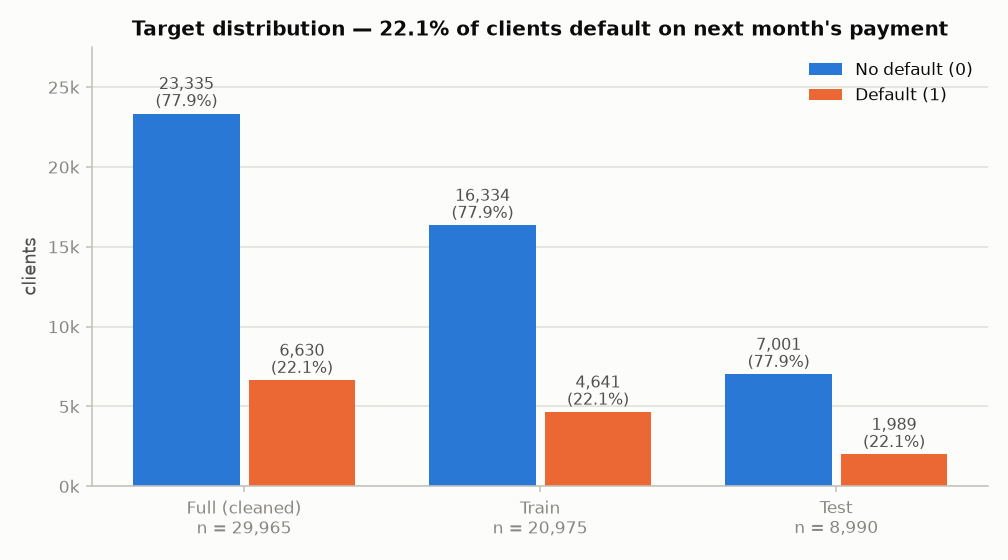
\includegraphics[width=0.92\linewidth]{eda_target_distribution.png}
  \caption{Class balance of the cleaned sample and of the stratified training and test partitions.}
  \label{fig:eda-target-distribution}
\end{figure}

\begin{figure}[htbp]
  \centering
  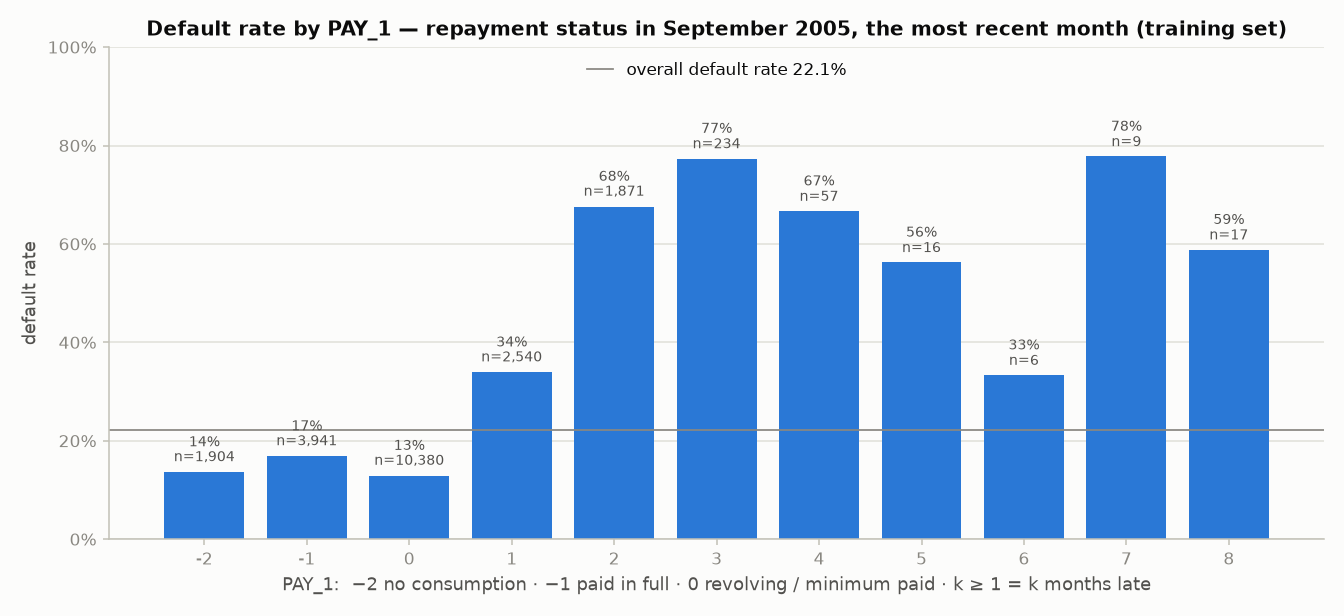
\includegraphics[width=0.92\linewidth]{eda_default_rate_by_pay1.png}
  \caption{Default rate by the most recent repayment status, training partition.}
  \label{fig:eda-default-rate-by-pay1}
\end{figure}

\begin{figure}[htbp]
  \centering
  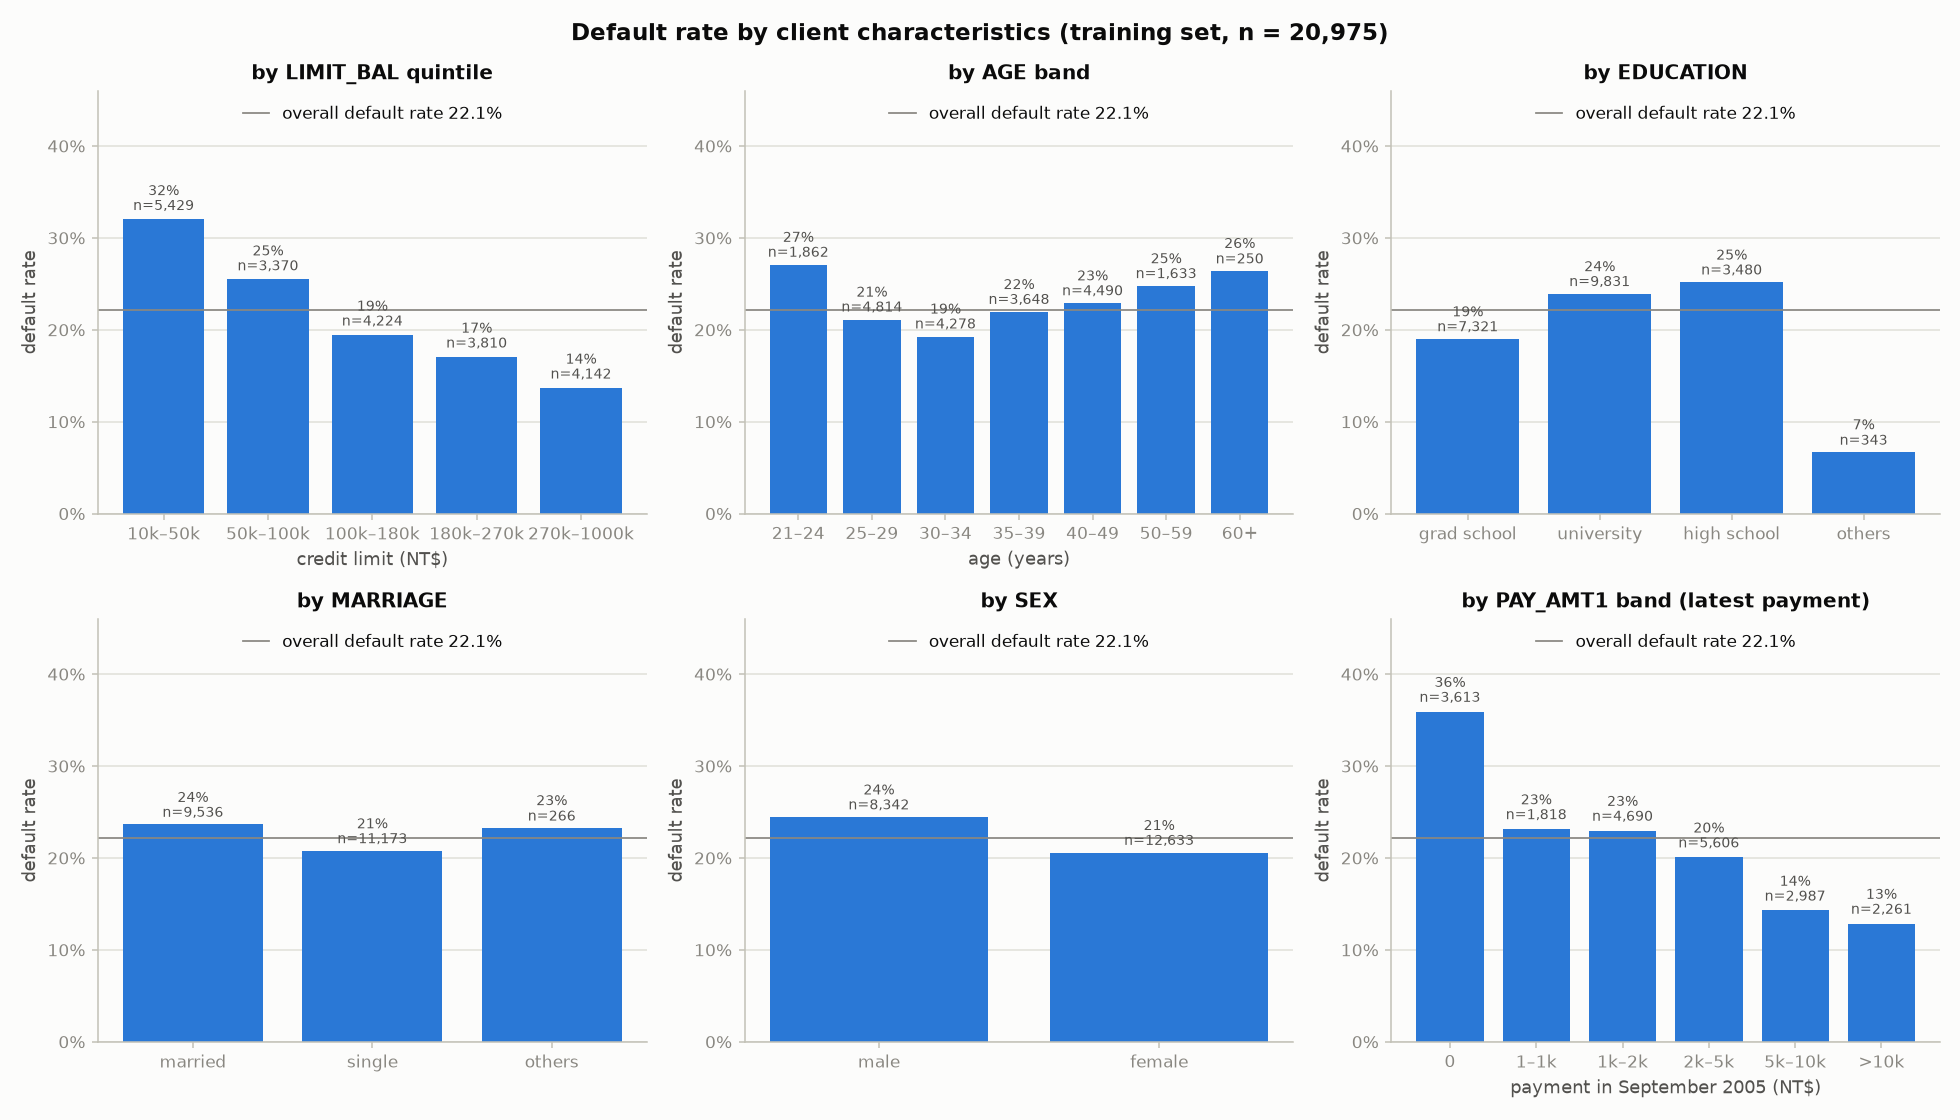
\includegraphics[width=0.92\linewidth]{eda_default_rate_by_groups.png}
  \caption{Training-partition default rate by credit-limit quintile, age band, education, marriage and sex.}
  \label{fig:eda-default-rate-by-groups}
\end{figure}

\begin{figure}[htbp]
  \centering
  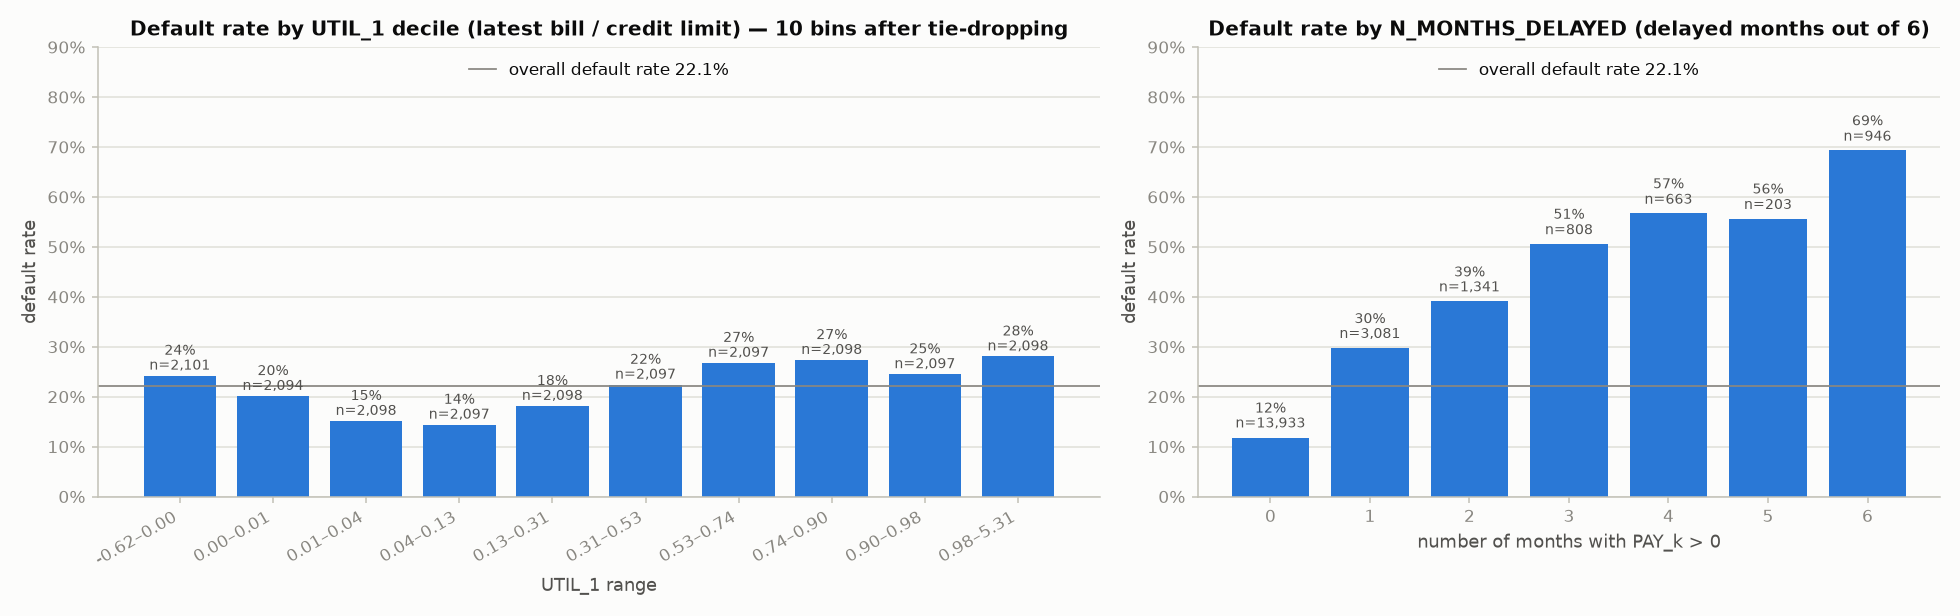
\includegraphics[width=0.92\linewidth]{eda_default_rate_util_delay.png}
  \caption{Default rate by utilisation decile and by number of months in arrears, training partition.}
  \label{fig:eda-default-rate-util-delay}
\end{figure}

\begin{figure}[p]
  \centering
  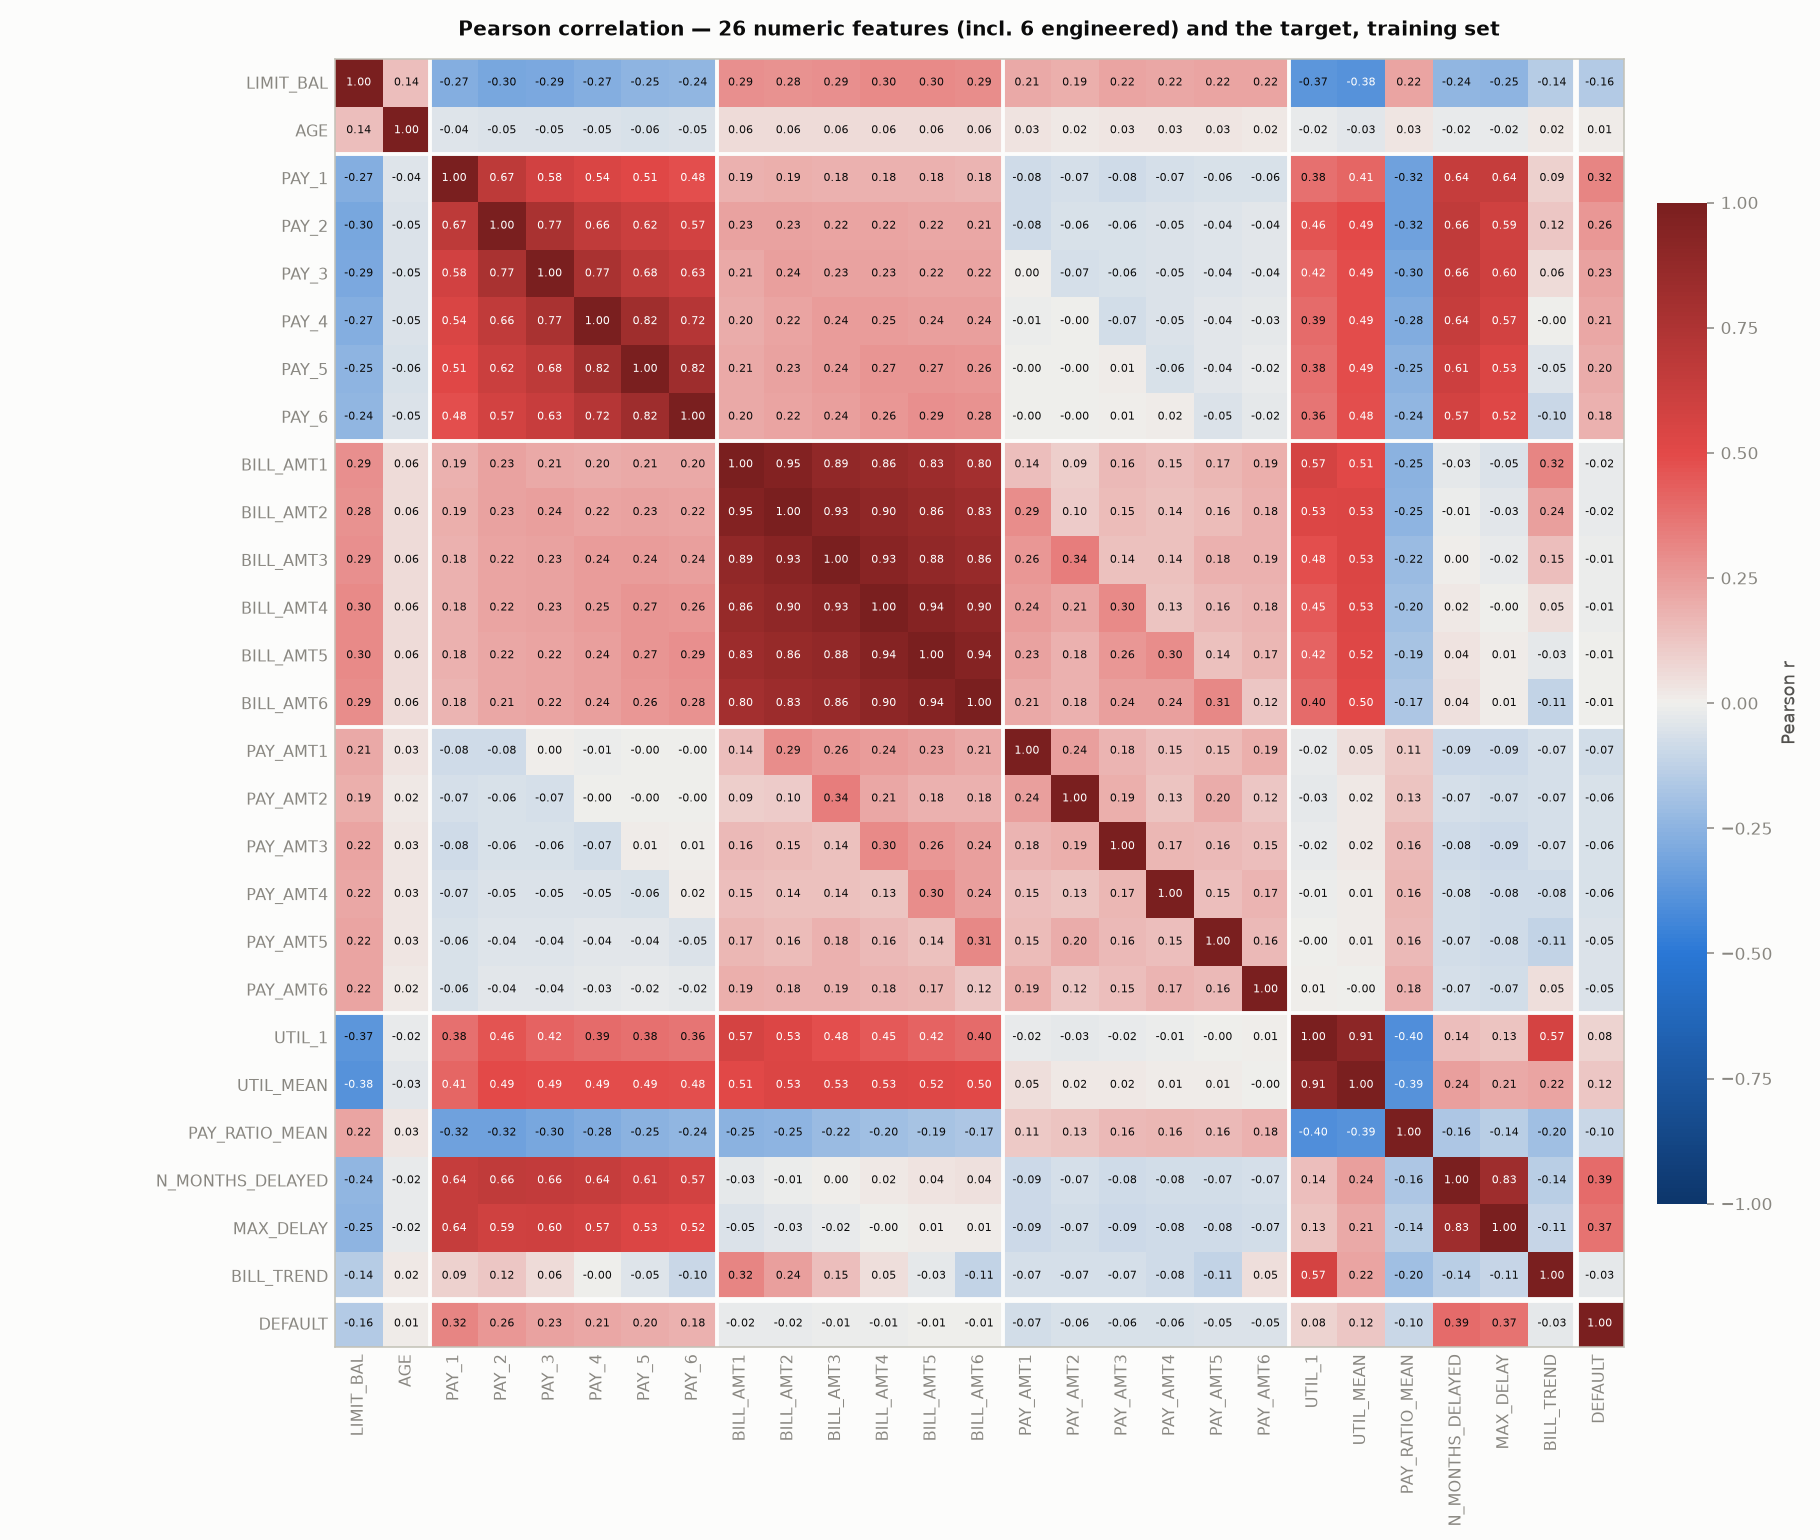
\includegraphics[width=1.0\linewidth]{eda_correlation_heatmap.png}
  \caption{Correlation heat-map of the 29 predictors and the target.}
  \label{fig:eda-correlation-heatmap}
\end{figure}

\begin{figure}[htbp]
  \centering
  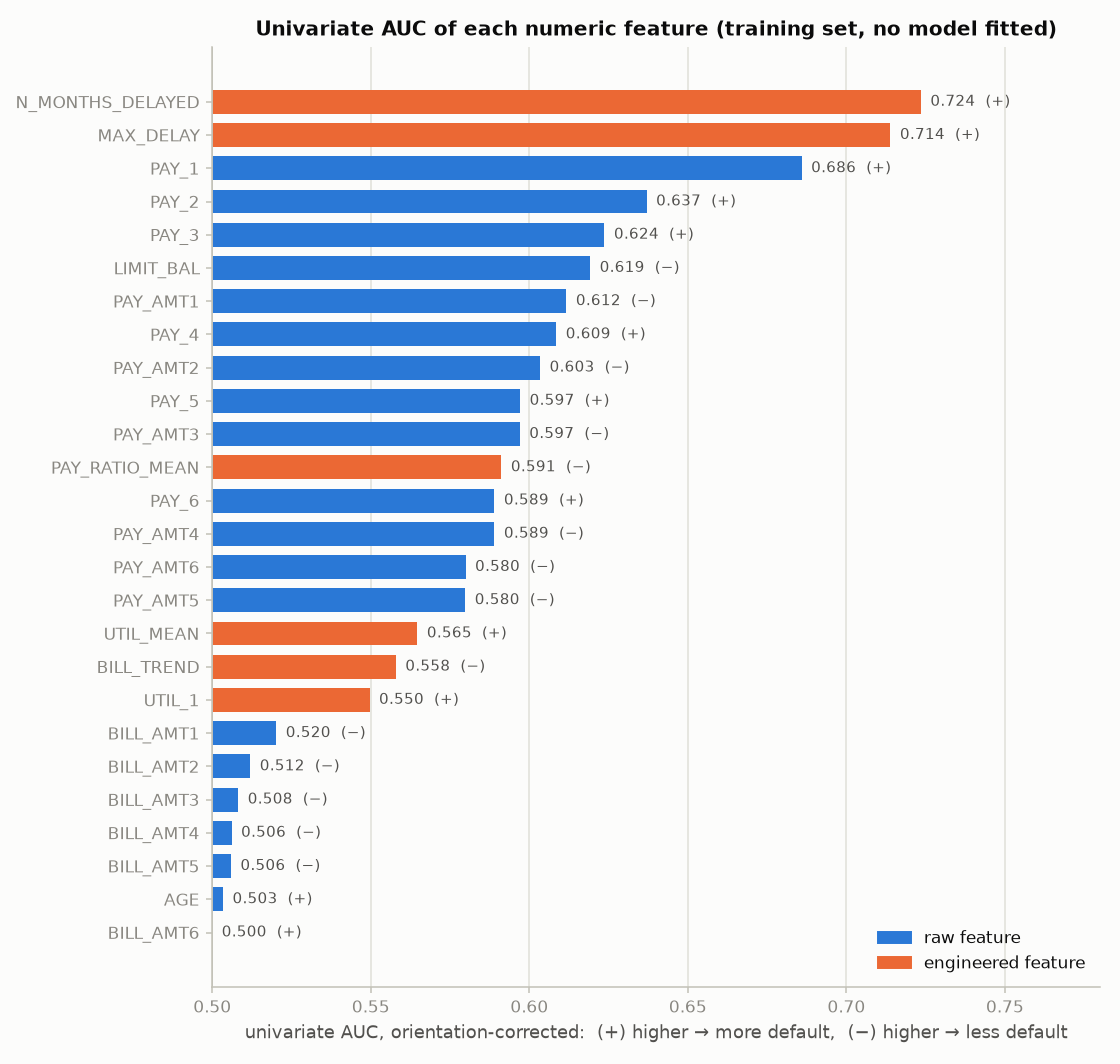
\includegraphics[width=0.92\linewidth]{eda_univariate_strength.png}
  \caption{Univariate strength of every predictor, as an oriented AUC.}
  \label{fig:eda-univariate-strength}
\end{figure}
\clearpage

\begin{figure}[htbp]
  \centering
  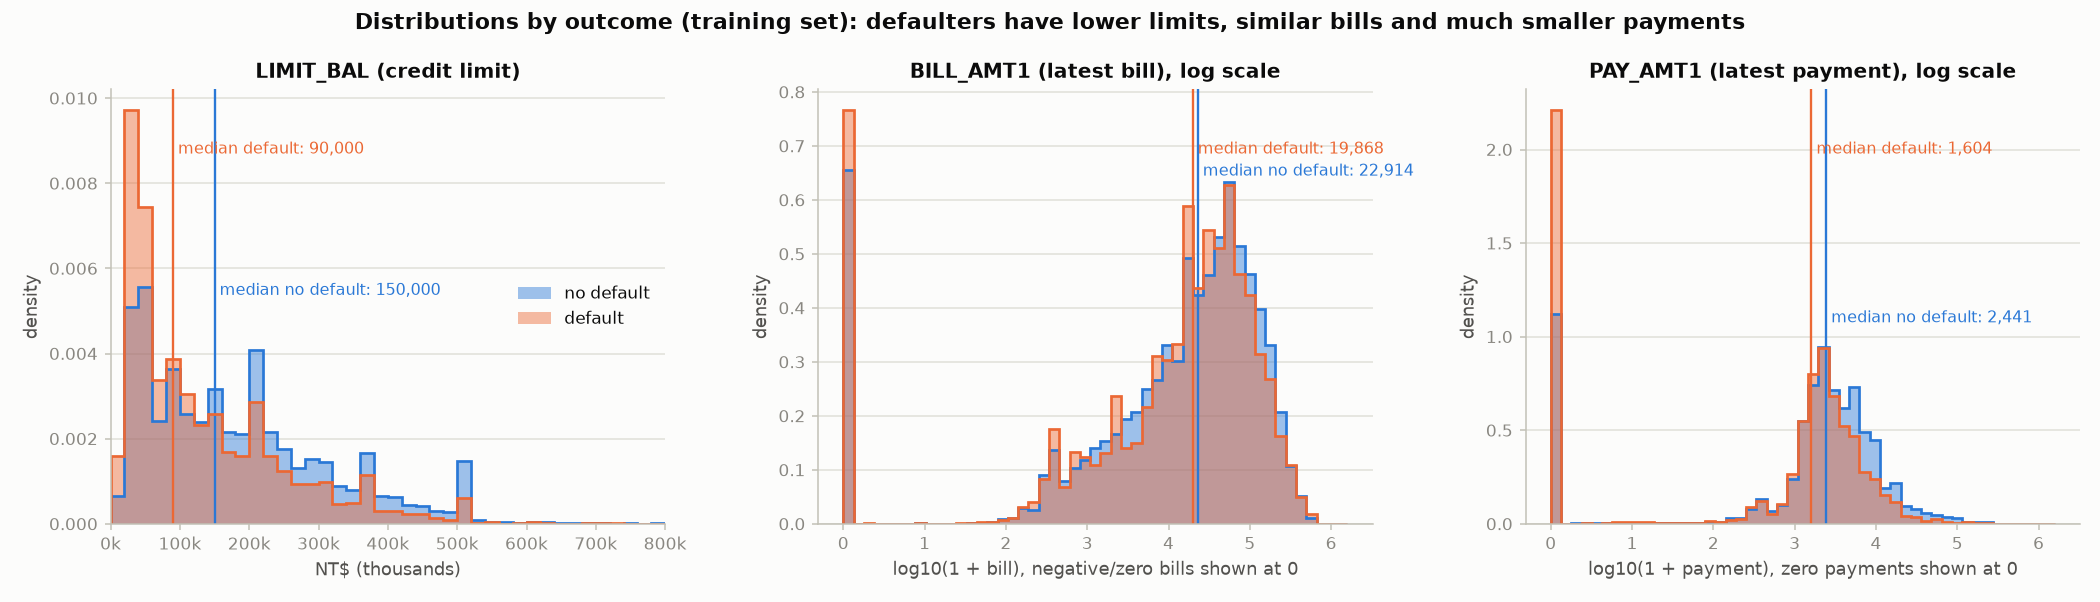
\includegraphics[width=0.92\linewidth]{eda_distributions_by_default.png}
  \caption{Distributions of the main numeric features by class, training partition.}
  \label{fig:eda-distributions-by-default}
\end{figure}

\clearpage
\subsection{Model comparison}

\begin{figure}[htbp]
  \centering
  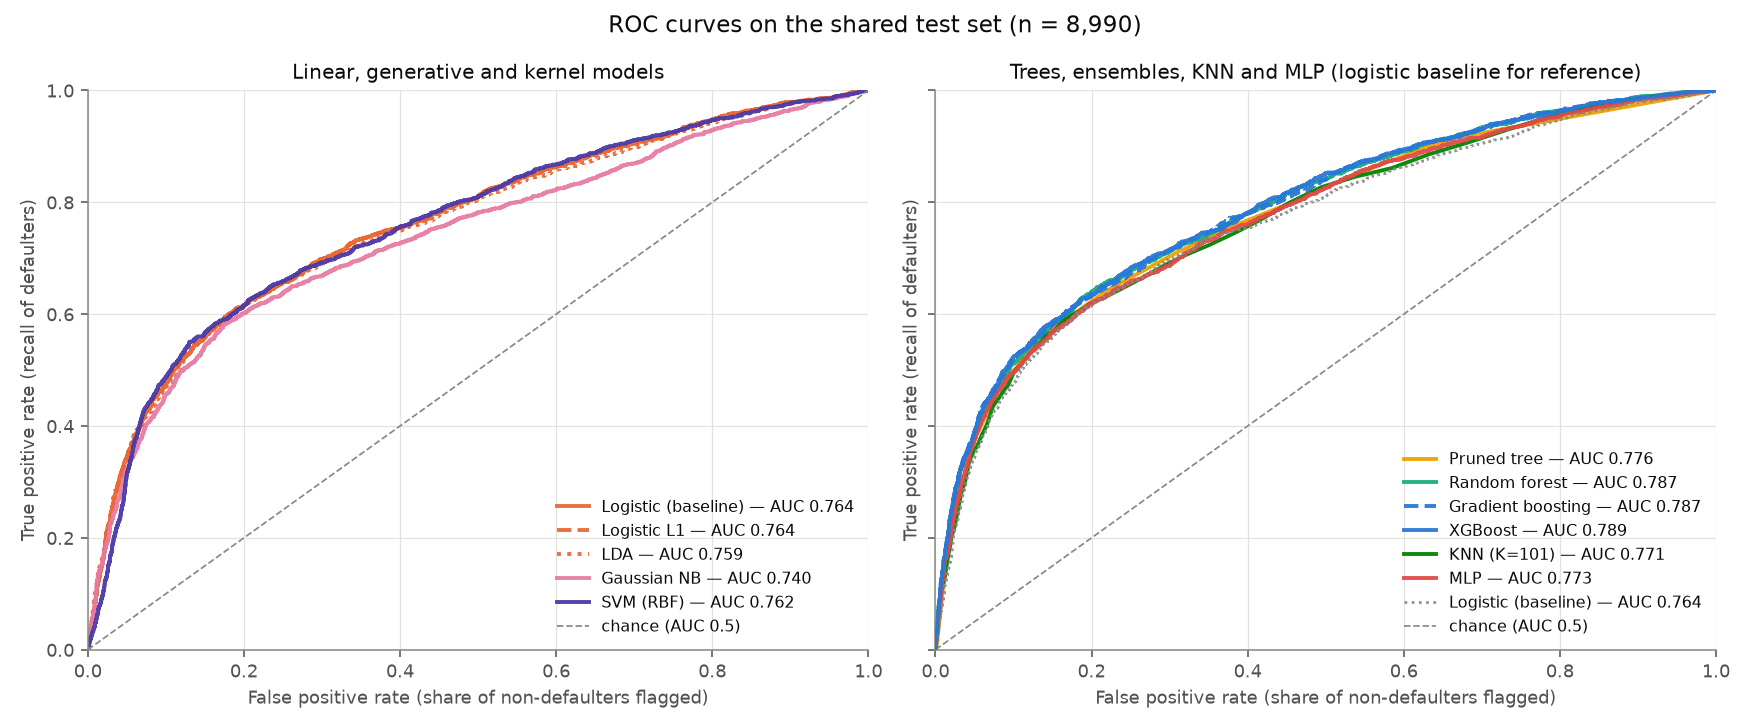
\includegraphics[width=0.92\linewidth]{all_roc.png}
  \caption{Test-set ROC curves of the headline models.}
  \label{fig:all-roc}
\end{figure}

\begin{figure}[htbp]
  \centering
  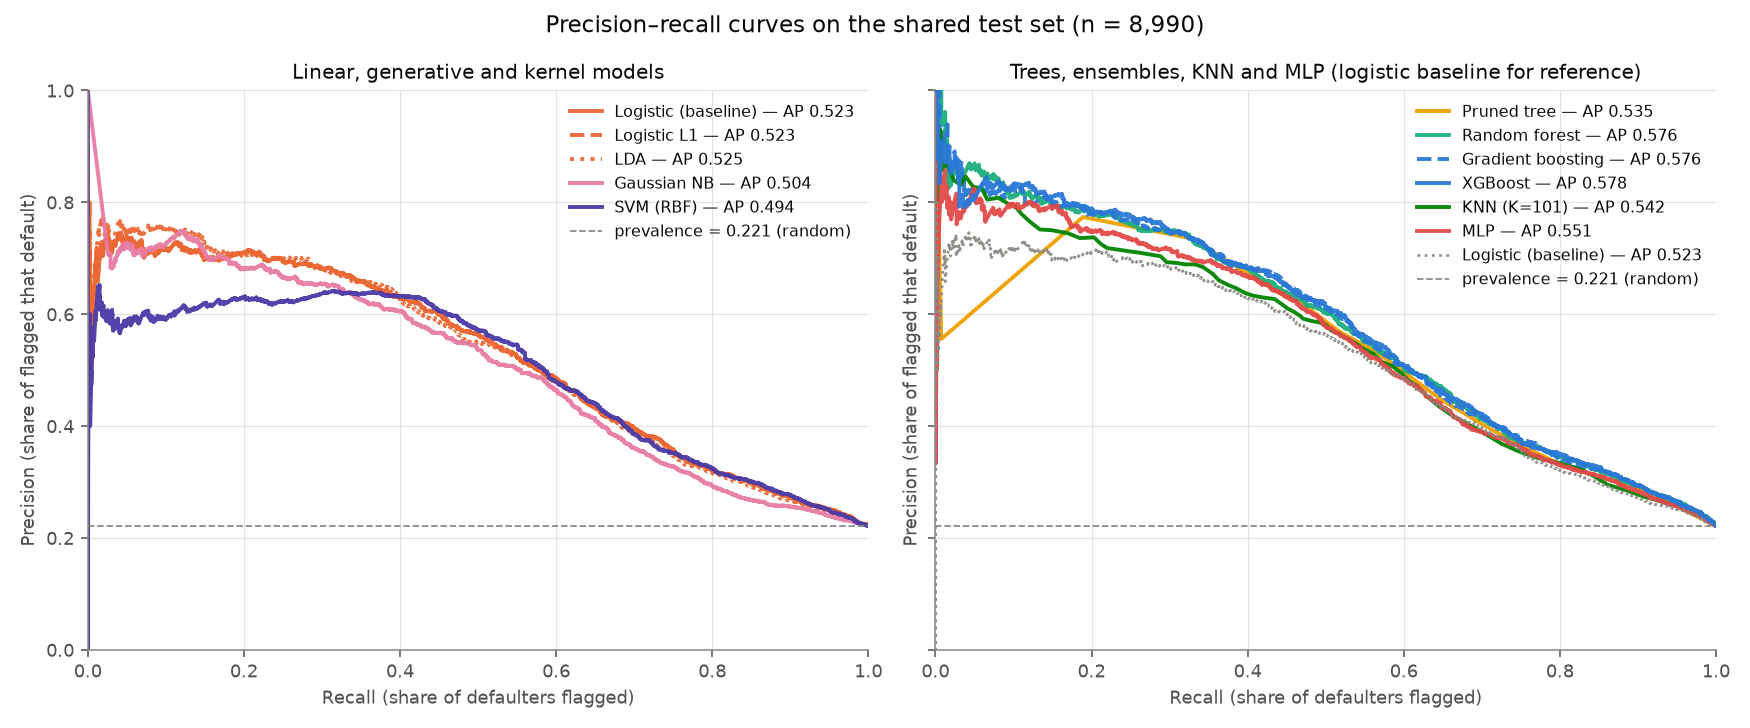
\includegraphics[width=0.92\linewidth]{all_pr.png}
  \caption{Test-set precision--recall curves; the horizontal line is the prevalence.}
  \label{fig:all-pr}
\end{figure}

\begin{figure}[htbp]
  \centering
  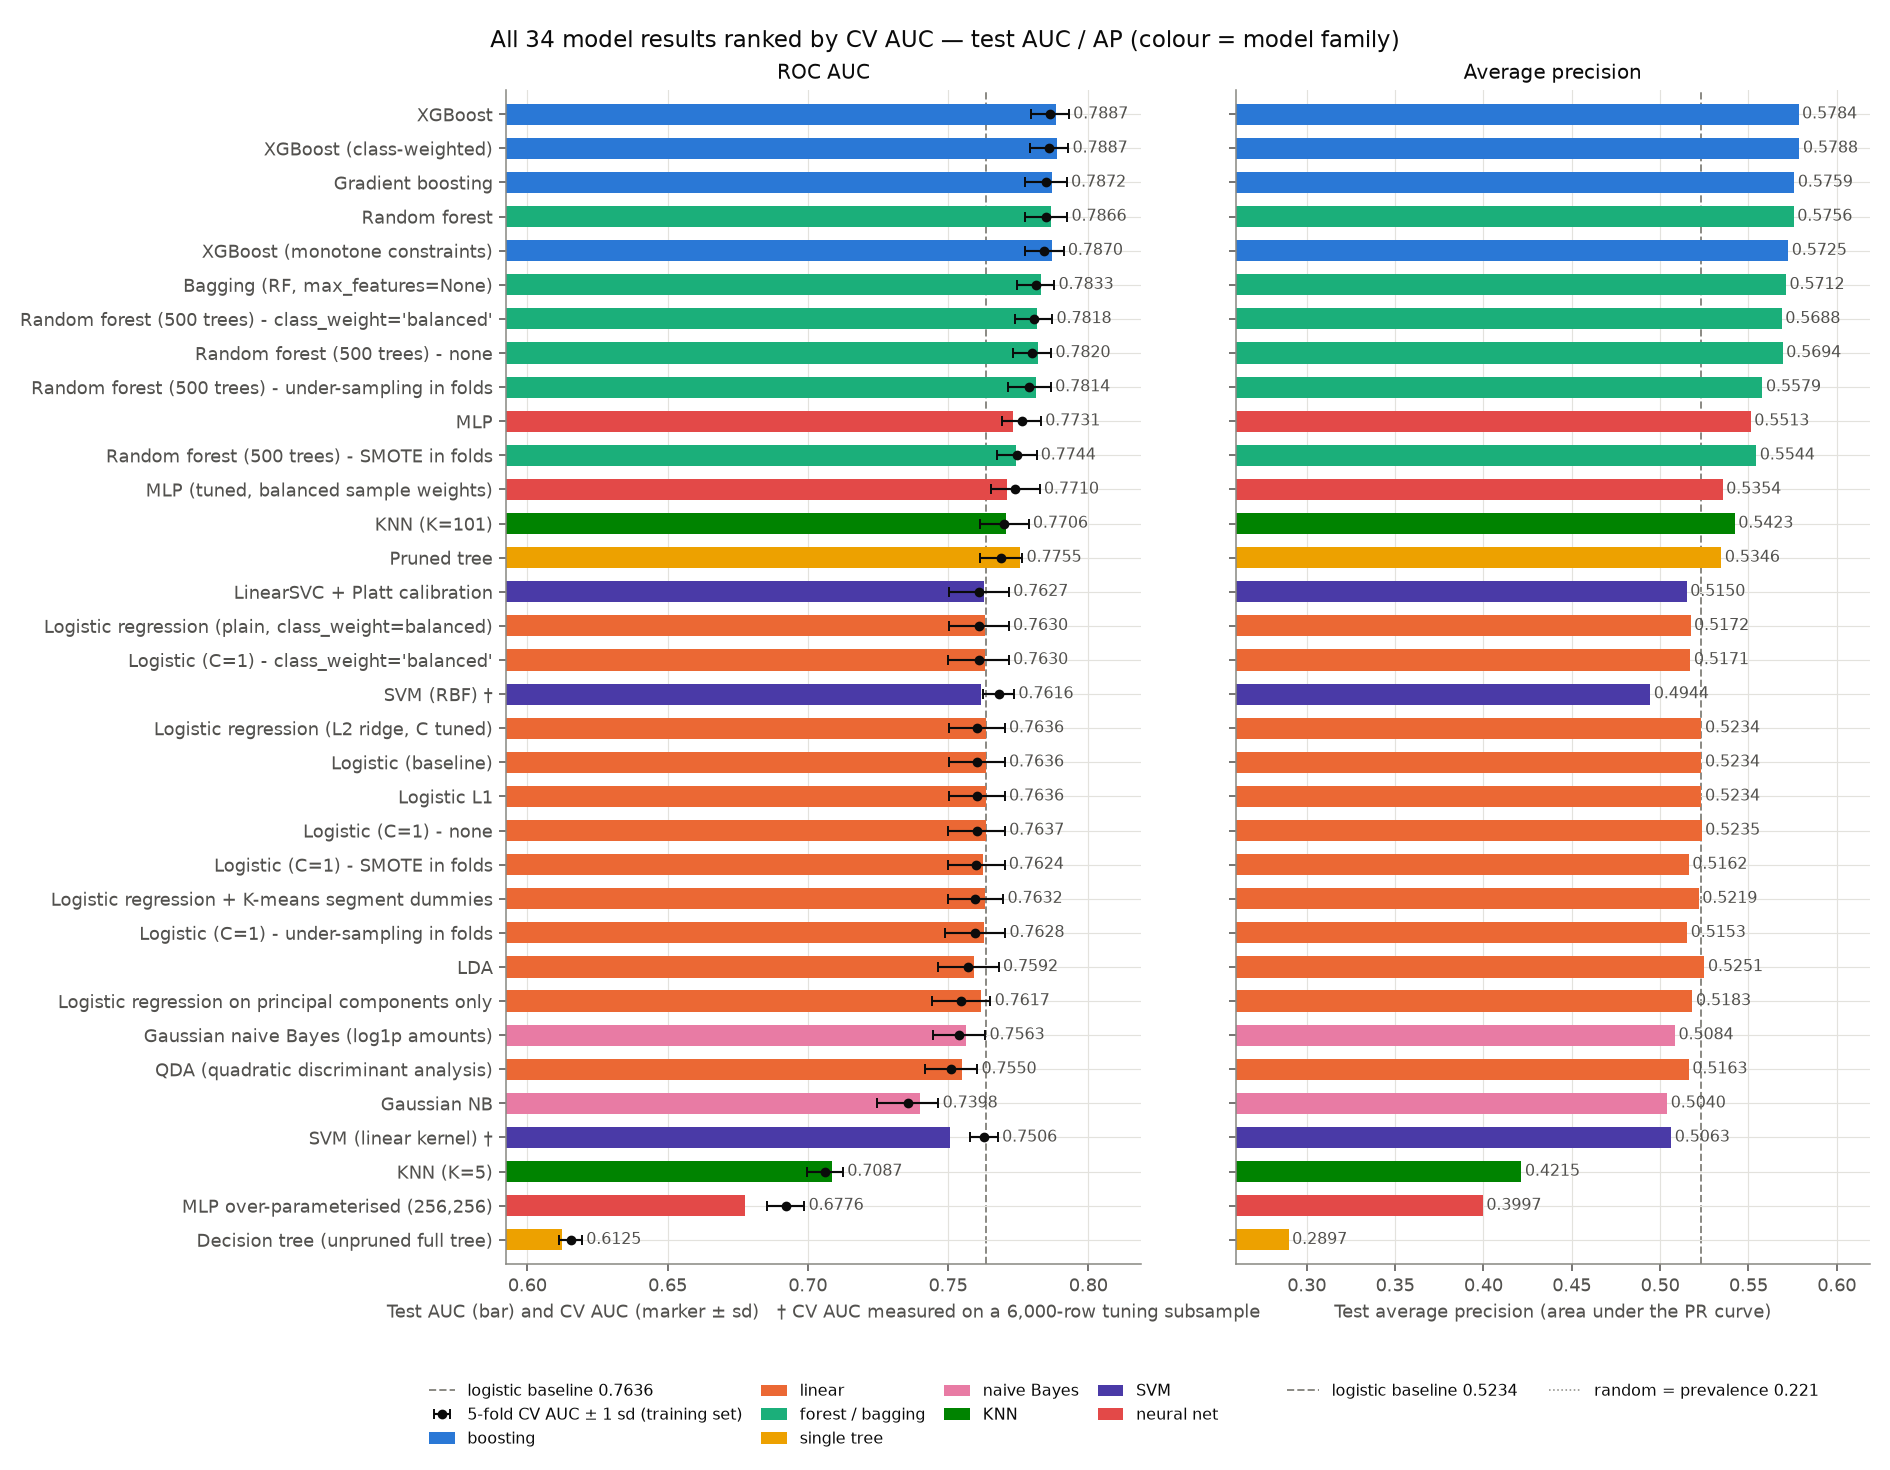
\includegraphics[width=0.92\linewidth]{all_auc_bar_full.png}
  \caption{Test AUC of every model variant fitted, ordered by CV AUC, with the benchmark marked.}
  \label{fig:all-auc-bar-full}
\end{figure}

\begin{figure}[htbp]
  \centering
  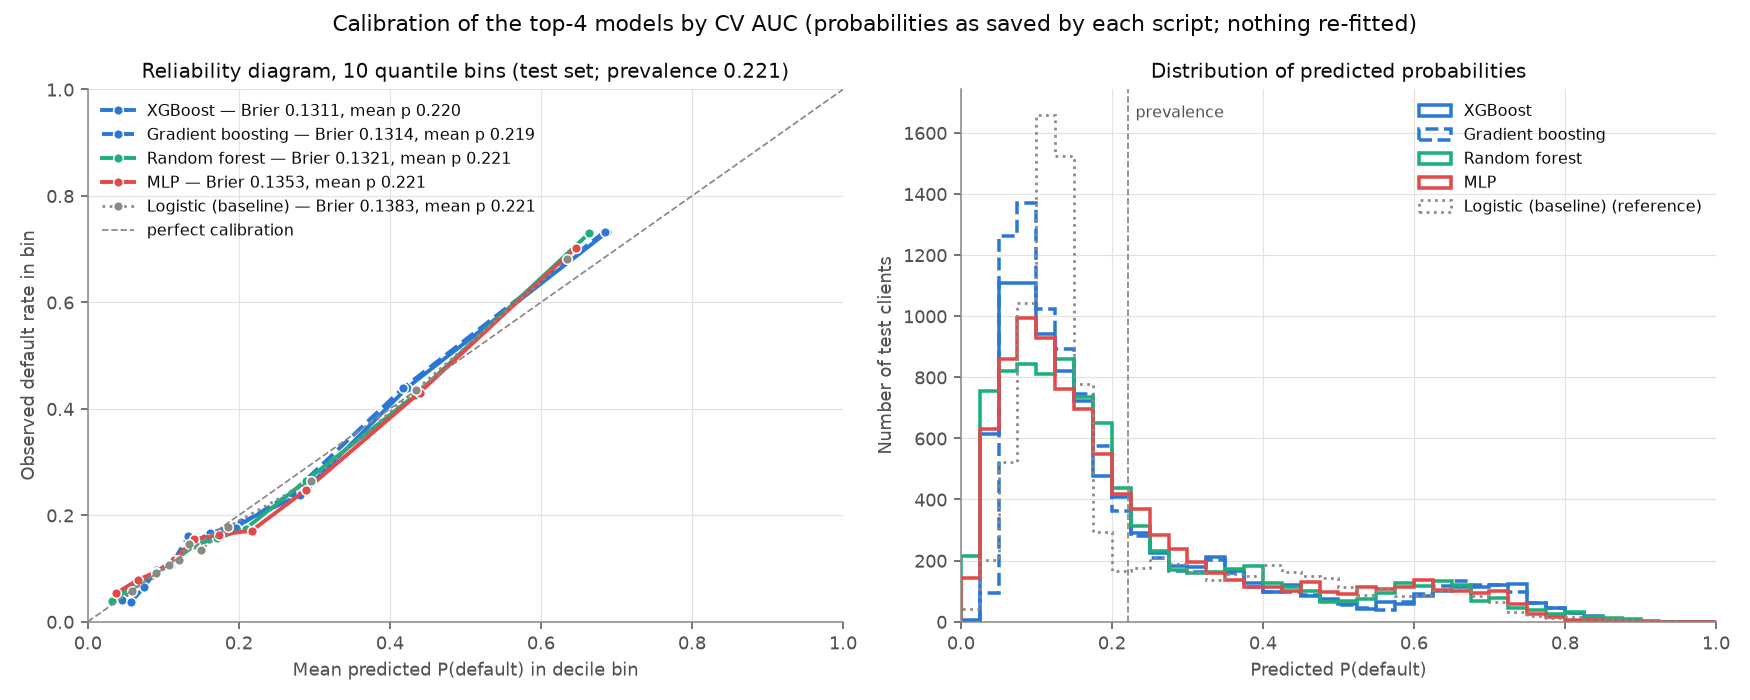
\includegraphics[width=0.92\linewidth]{calibration.png}
  \caption{Calibration curves of the four models with the highest CV AUC: predicted against observed default rate by decile of score.}
  \label{fig:calibration}
\end{figure}

\begin{figure}[htbp]
  \centering
  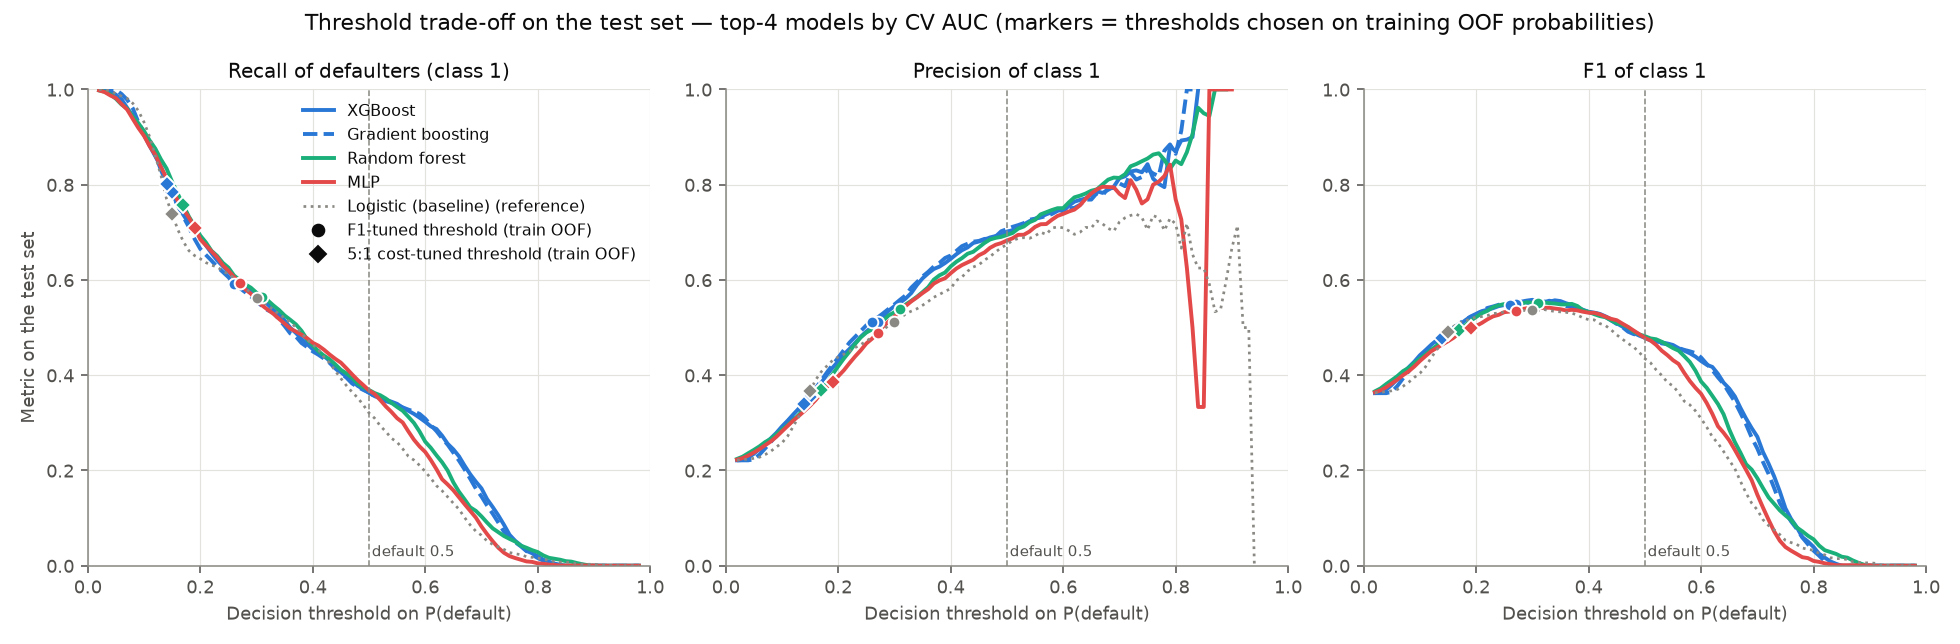
\includegraphics[width=0.92\linewidth]{threshold_curves.png}
  \caption{Recall, precision and F1 against the decision threshold.}
  \label{fig:threshold-curves}
\end{figure}
\clearpage

\begin{figure}[htbp]
  \centering
  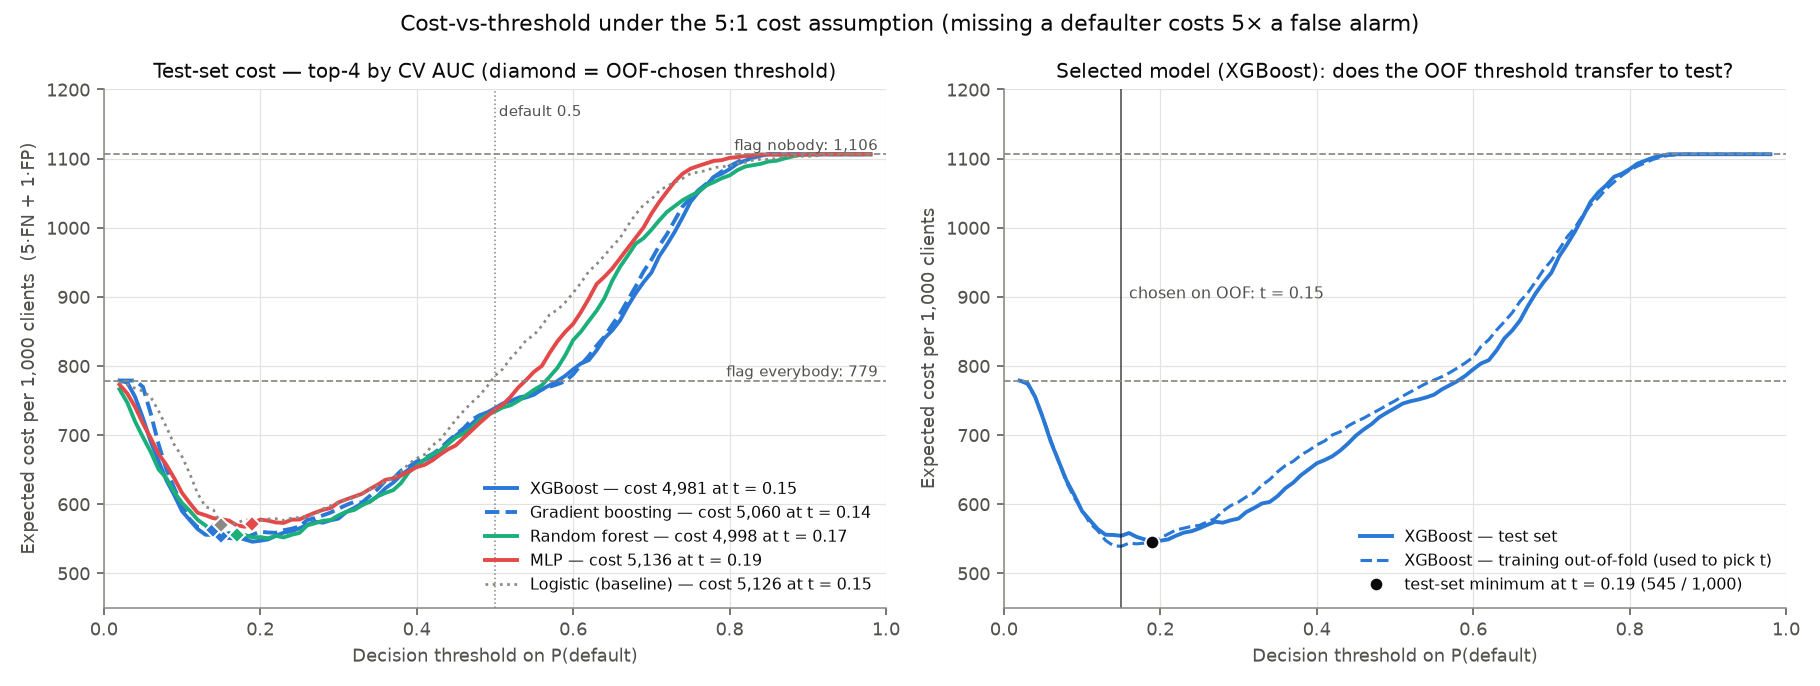
\includegraphics[width=0.92\linewidth]{cost_curves.png}
  \caption{Expected cost against the decision threshold at a 5:1 ratio.}
  \label{fig:cost-curves}
\end{figure}

\begin{figure}[htbp]
  \centering
  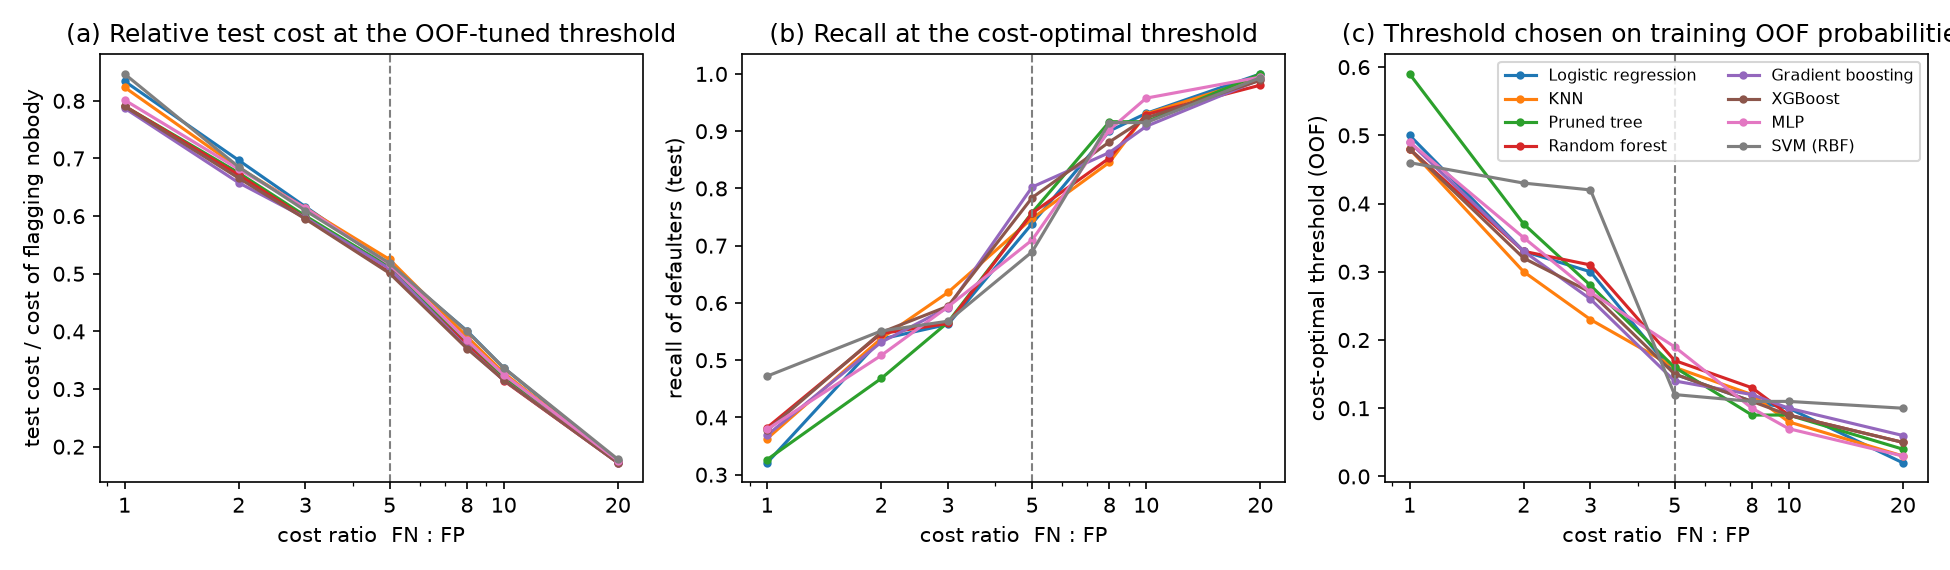
\includegraphics[width=0.92\linewidth]{cost_sensitivity.png}
  \caption{Cost-minimising threshold and cost as the cost ratio varies from 1:1 to 20:1.}
  \label{fig:cost-sensitivity}
\end{figure}

\begin{figure}[htbp]
  \centering
  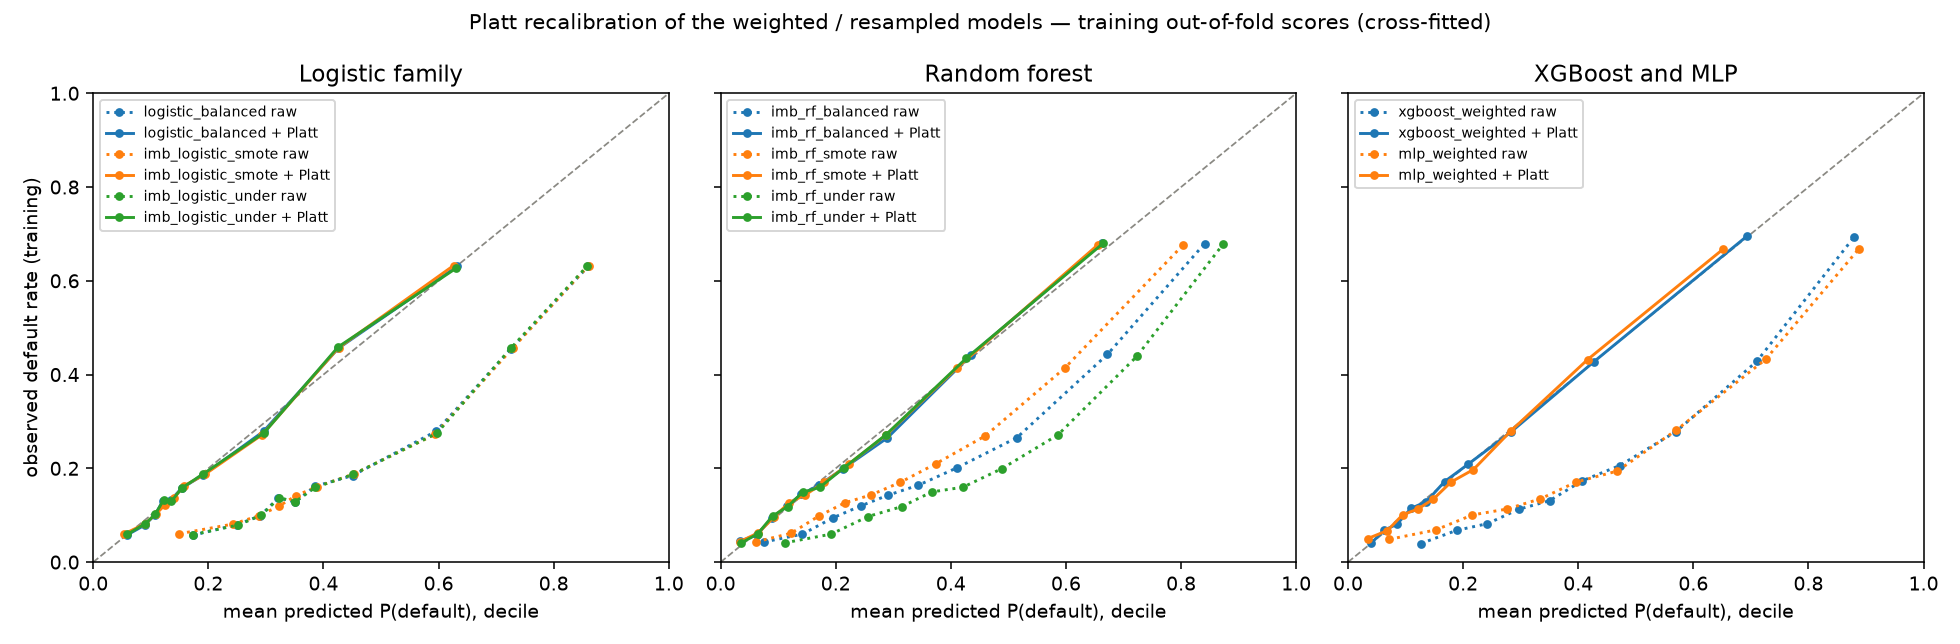
\includegraphics[width=0.92\linewidth]{recalibration.png}
  \caption{Reliability of the nine weighted or resampled models before and after Platt recalibration, on training out-of-fold scores.}
  \label{fig:recalibration}
\end{figure}

\clearpage
\subsection{Interpretation}

\begin{figure}[htbp]
  \centering
  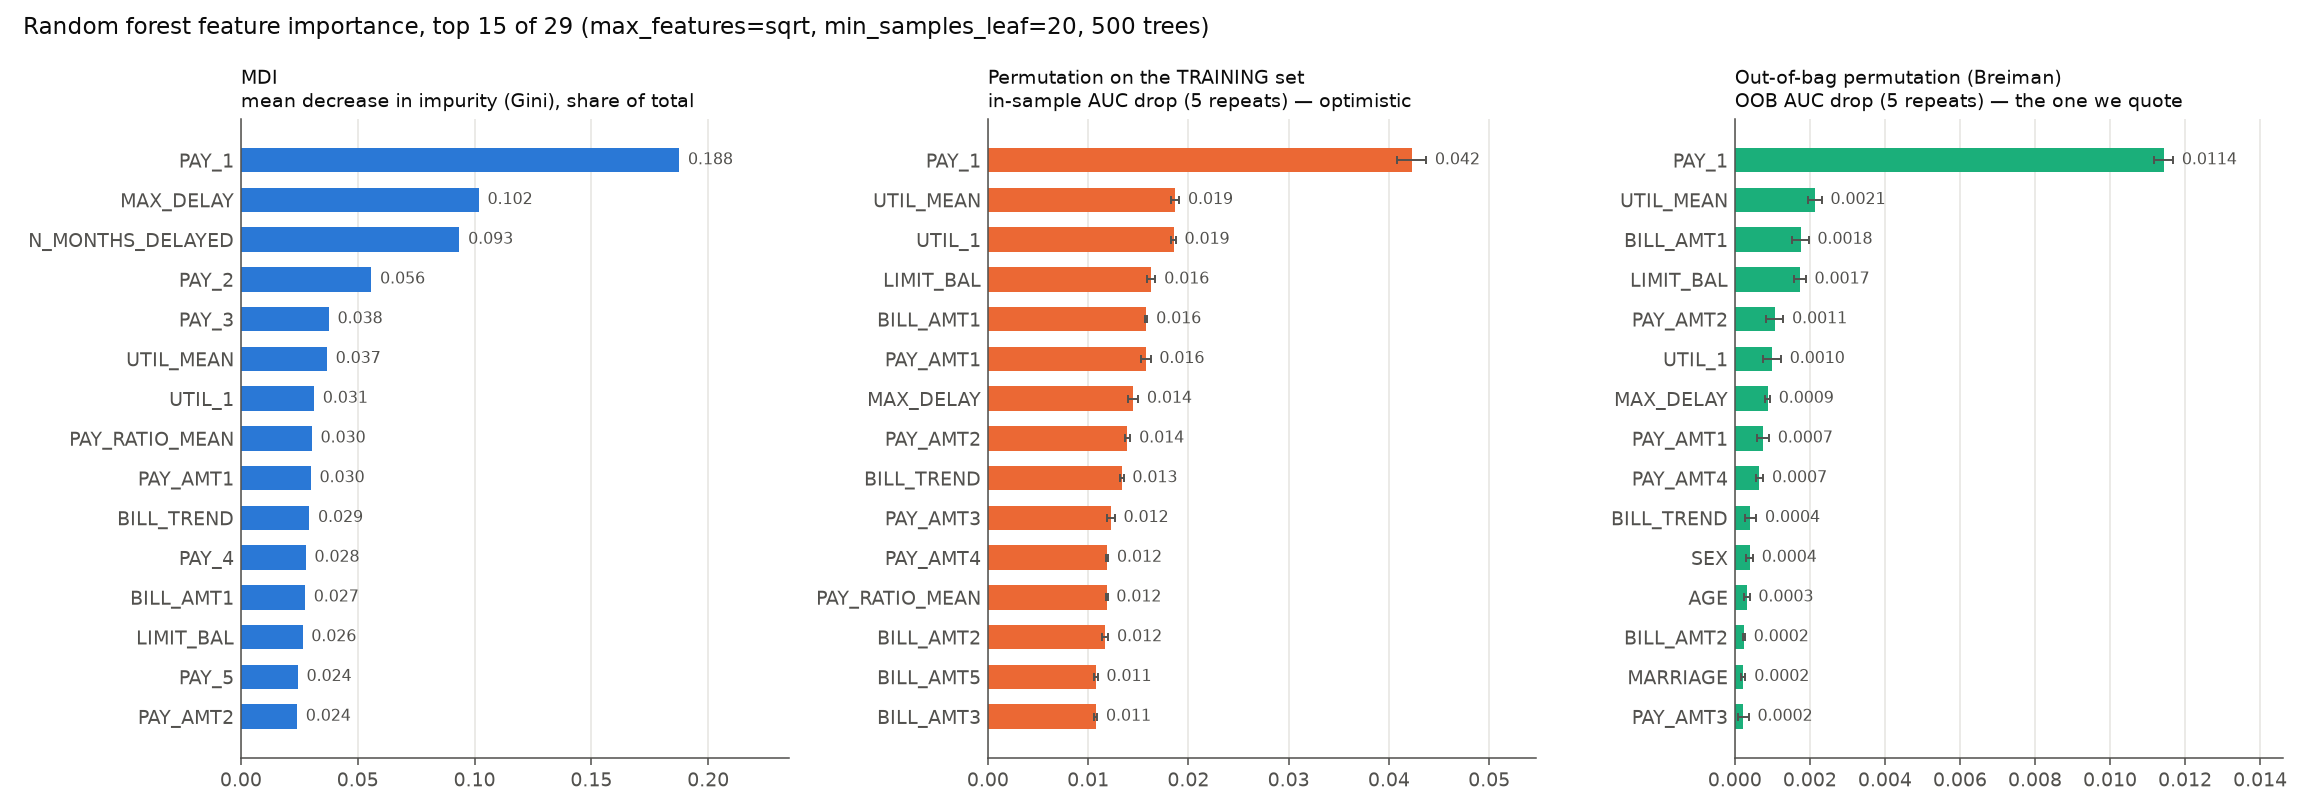
\includegraphics[width=0.92\linewidth]{rf_importance.png}
  \caption{Random forest importances: impurity decrease, training-set permutation and out-of-bag permutation, side by side.}
  \label{fig:rf-importance}
\end{figure}

\begin{figure}[htbp]
  \centering
  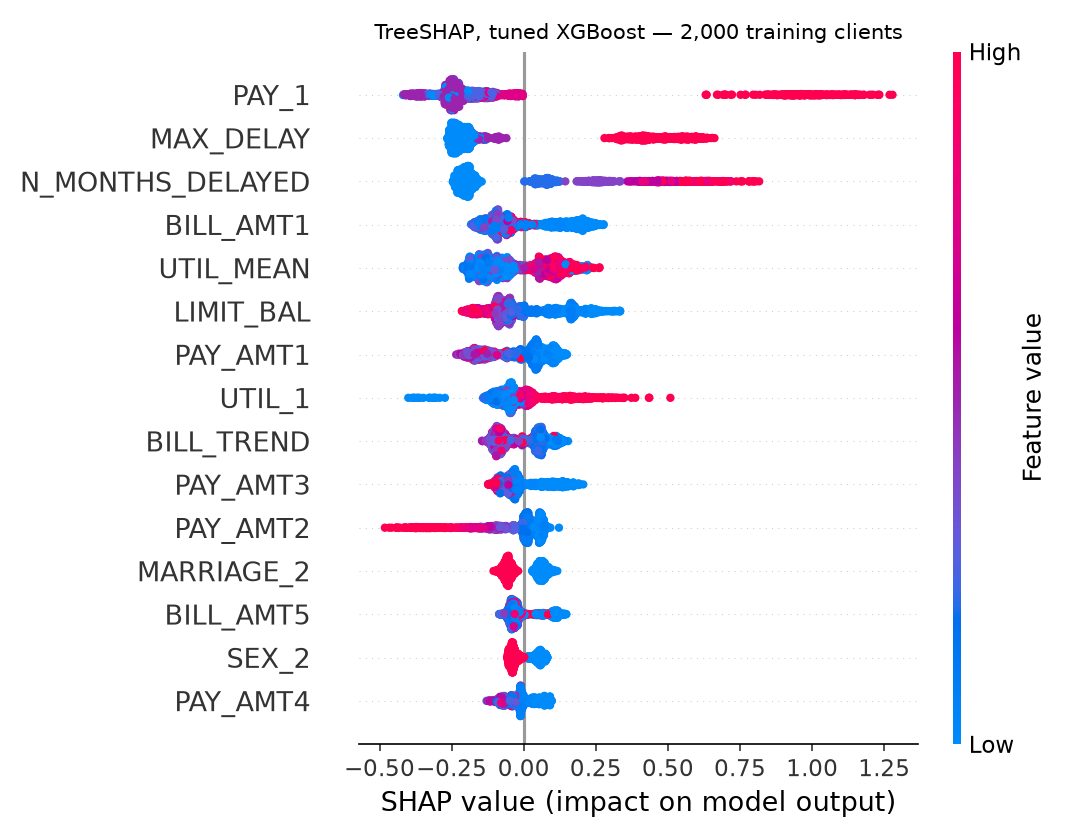
\includegraphics[width=0.92\linewidth]{shap_beeswarm.png}
  \caption{TreeSHAP beeswarm for the tuned XGBoost over training clients.}
  \label{fig:shap-beeswarm}
\end{figure}

\begin{figure}[htbp]
  \centering
  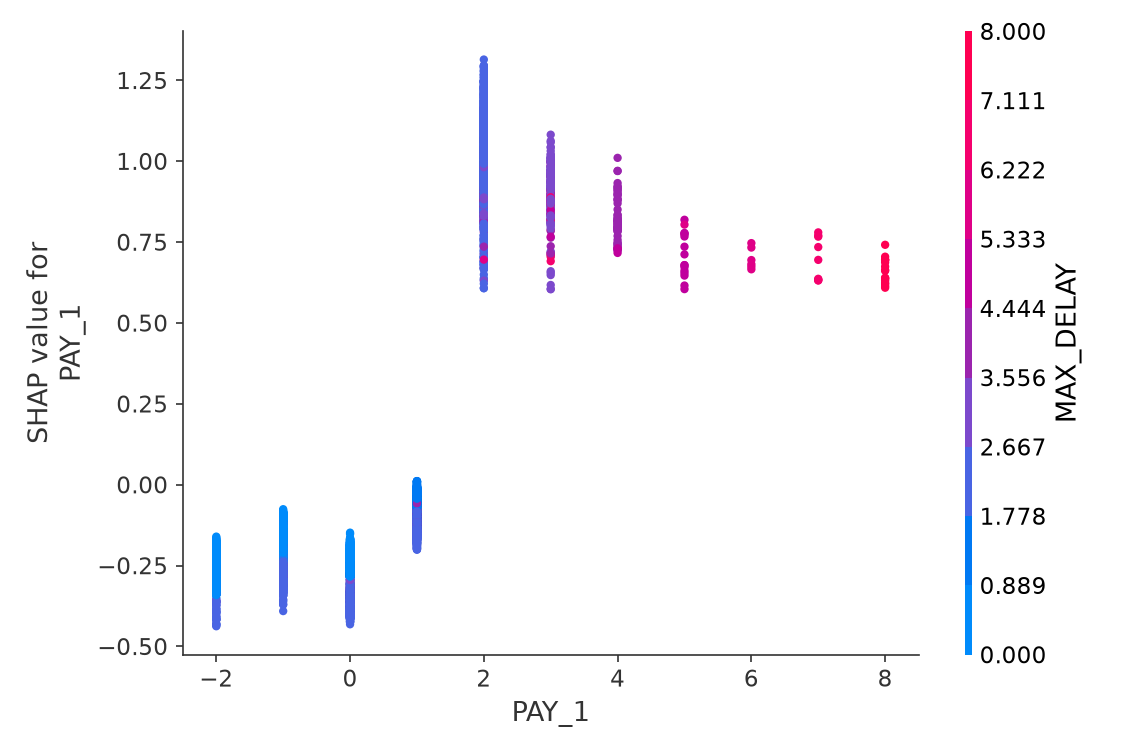
\includegraphics[width=0.92\linewidth]{shap_dependence_pay1.png}
  \caption{TreeSHAP dependence plot for the most recent repayment status.}
  \label{fig:shap-dependence-pay1}
\end{figure}
\clearpage

\begin{figure}[htbp]
  \centering
  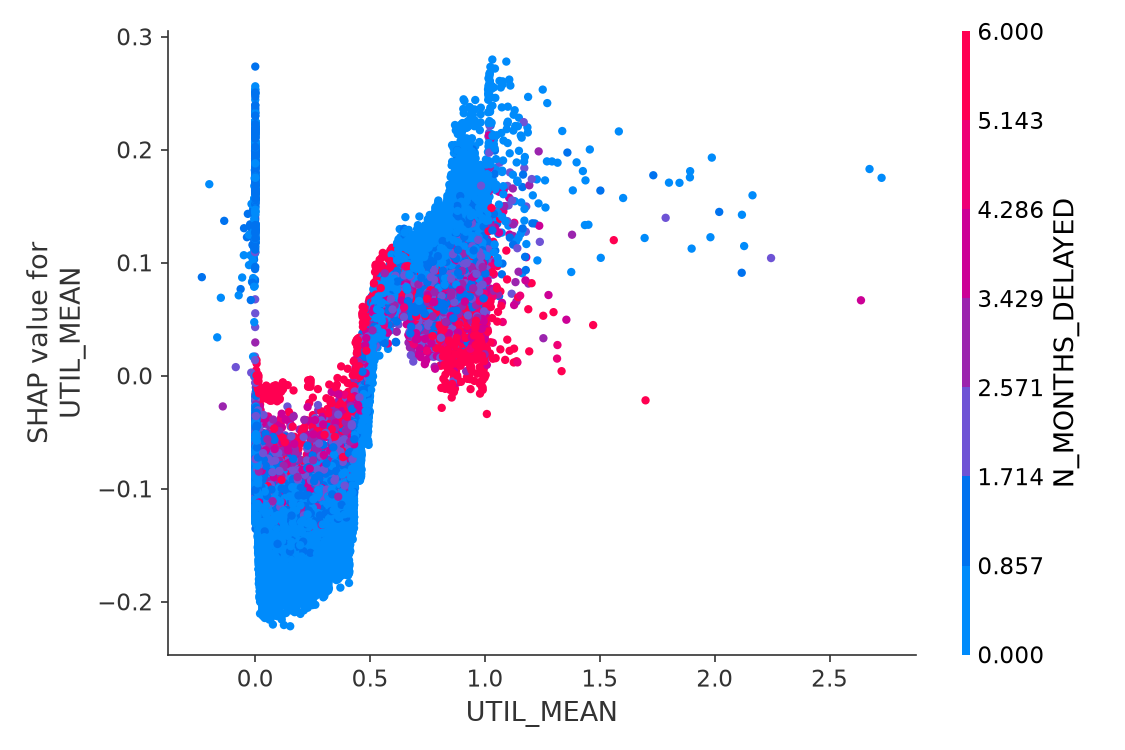
\includegraphics[width=0.92\linewidth]{shap_dependence_util_mean.png}
  \caption{TreeSHAP dependence plot for mean utilisation.}
  \label{fig:shap-dependence-util-mean}
\end{figure}

\begin{figure}[htbp]
  \centering
  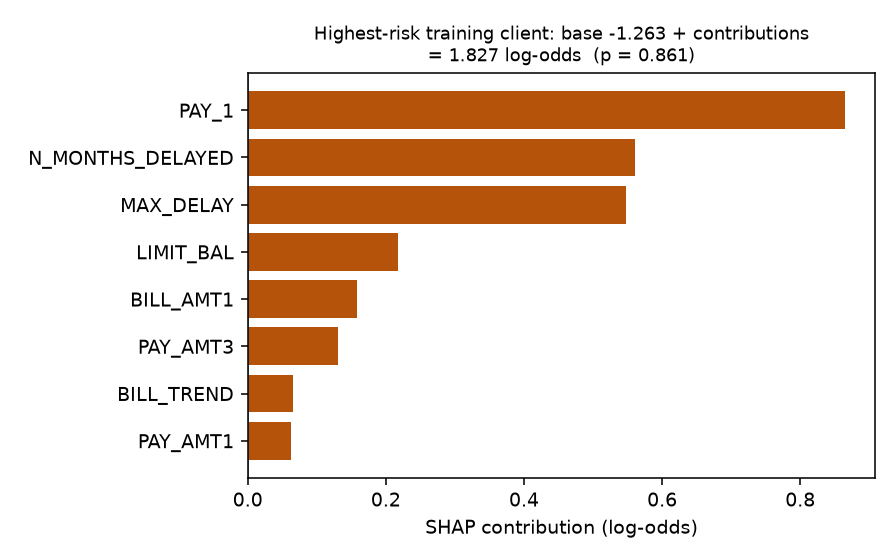
\includegraphics[width=0.92\linewidth]{shap_waterfall.png}
  \caption{One client decomposed: base value plus each feature's contribution.}
  \label{fig:shap-waterfall}
\end{figure}

\begin{figure}[p]
  \centering
  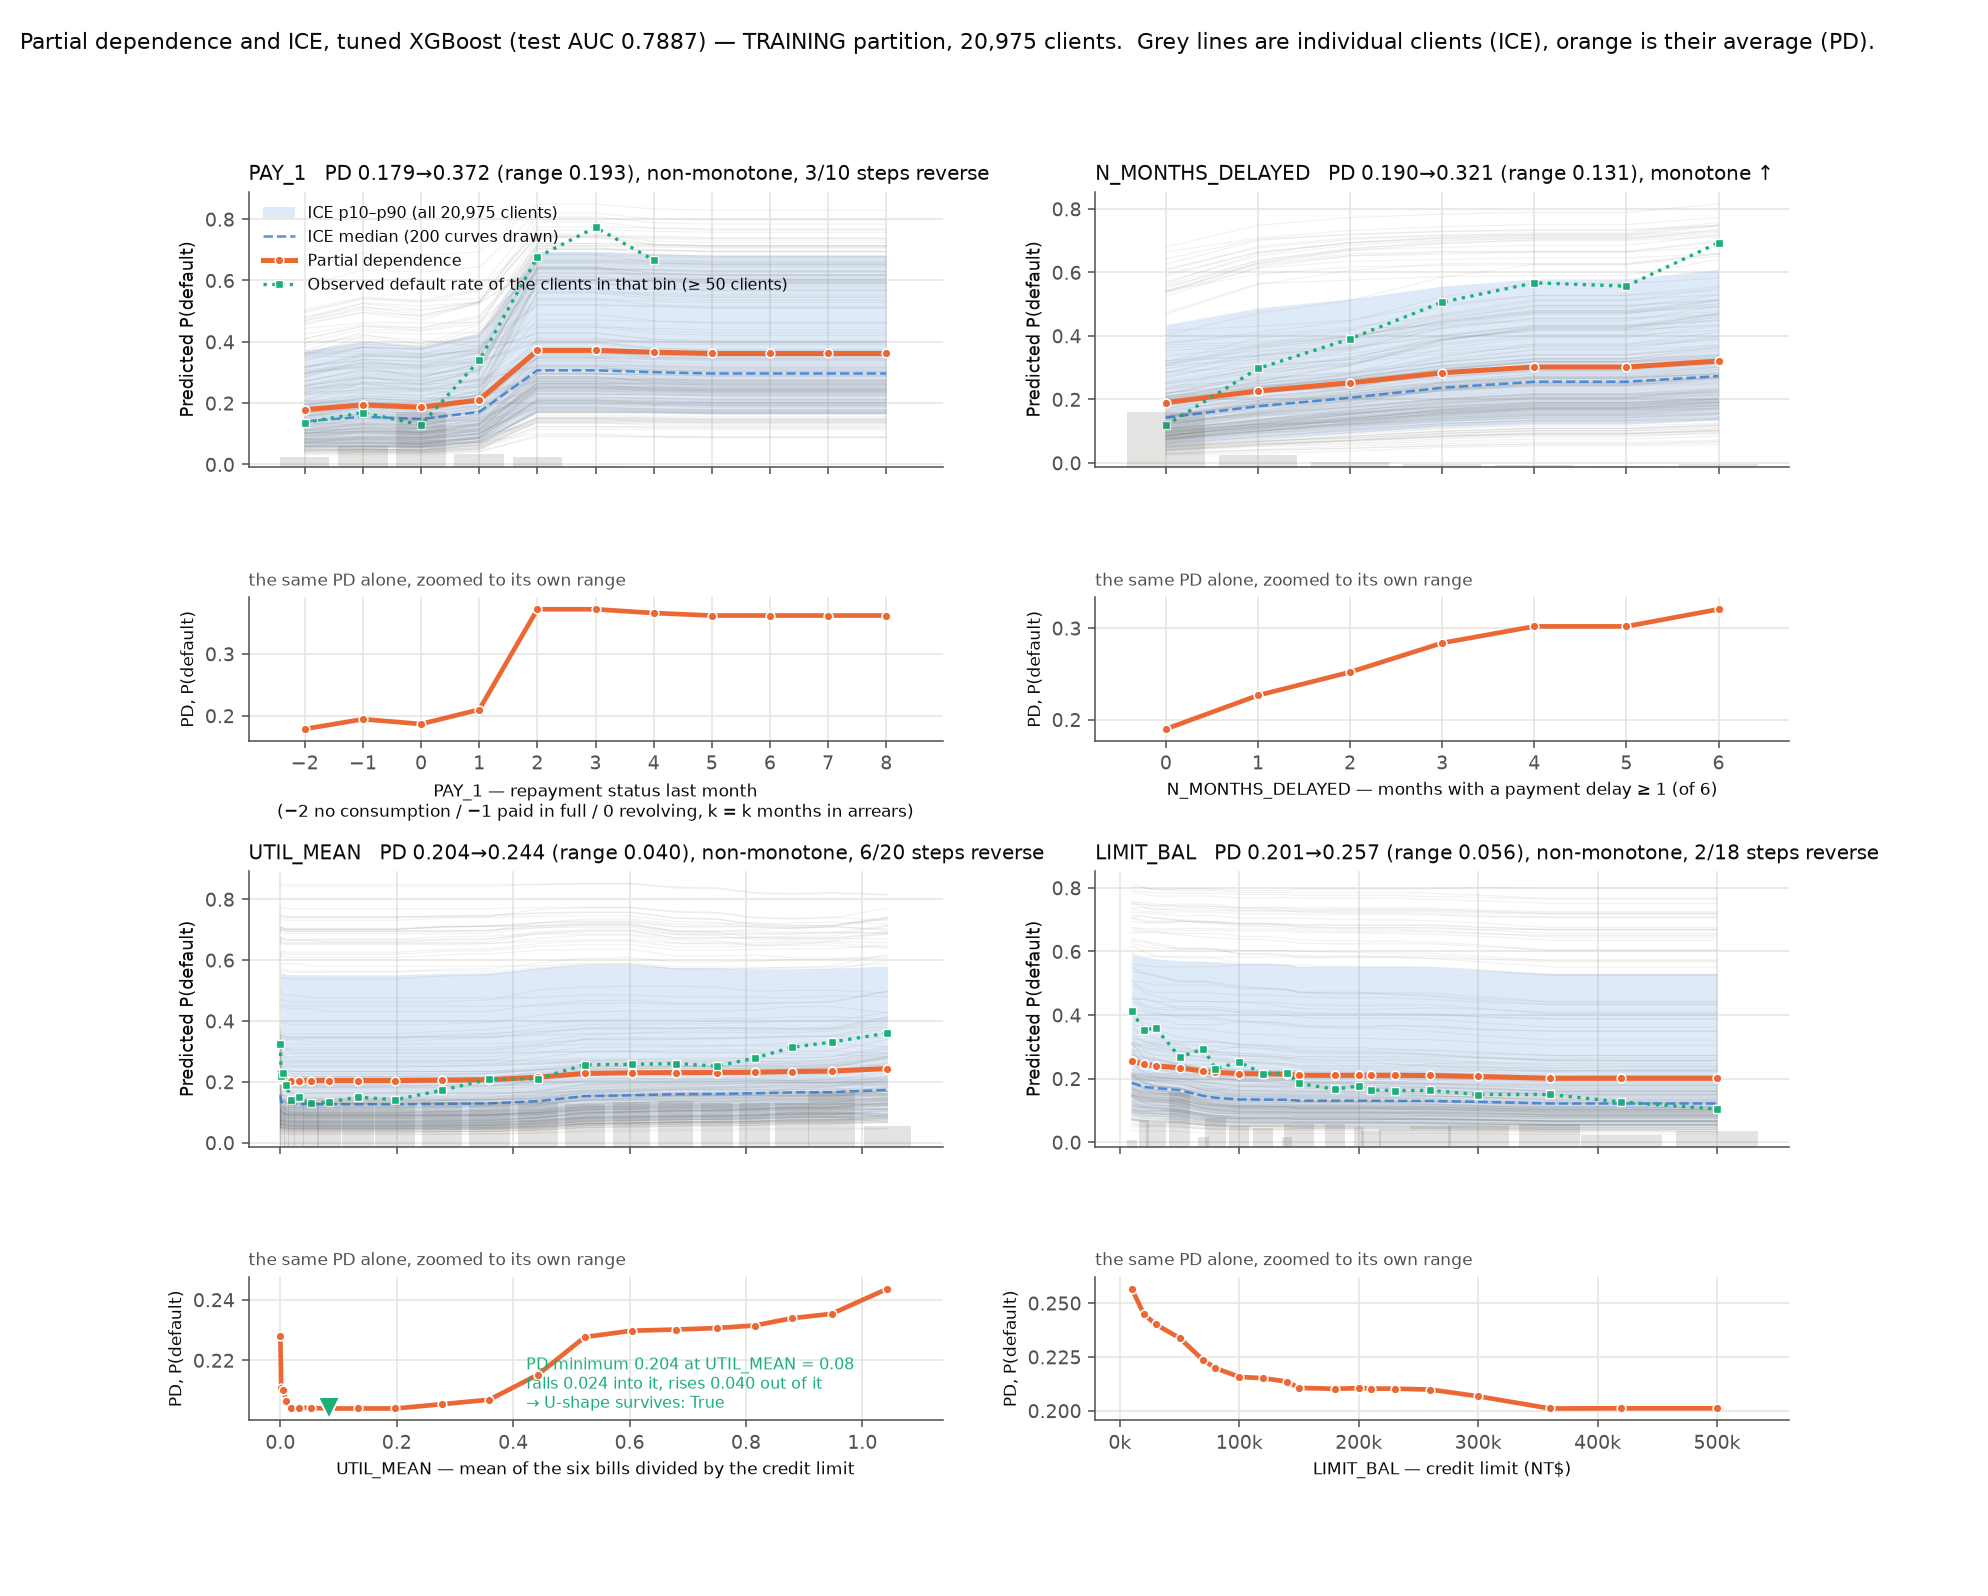
\includegraphics[width=1.0\linewidth]{pdp_main.png}
  \caption{Partial dependence with ICE curves for the four features that matter.}
  \label{fig:pdp-main}
\end{figure}

\begin{figure}[p]
  \centering
  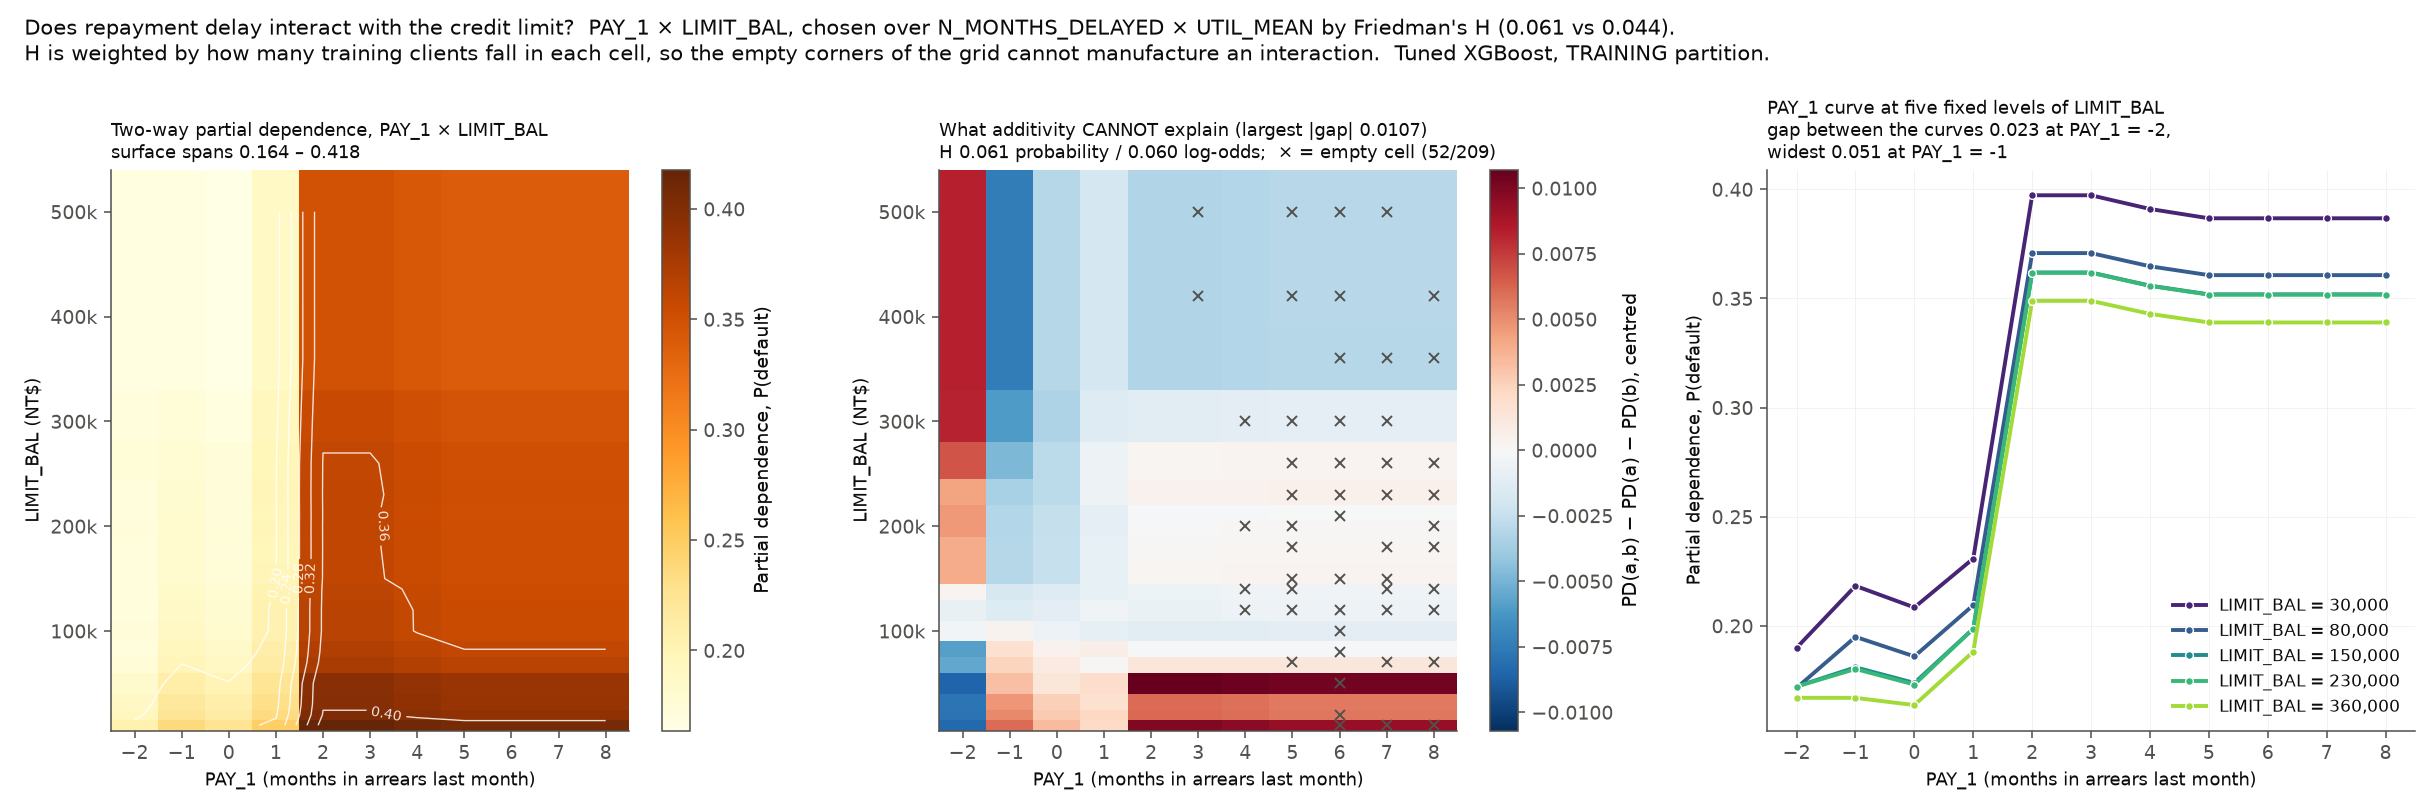
\includegraphics[width=1.0\linewidth]{pdp_interaction.png}
  \caption{Two-way partial dependence; cells with no training client are crossed.}
  \label{fig:pdp-interaction}
\end{figure}

\begin{figure}[htbp]
  \centering
  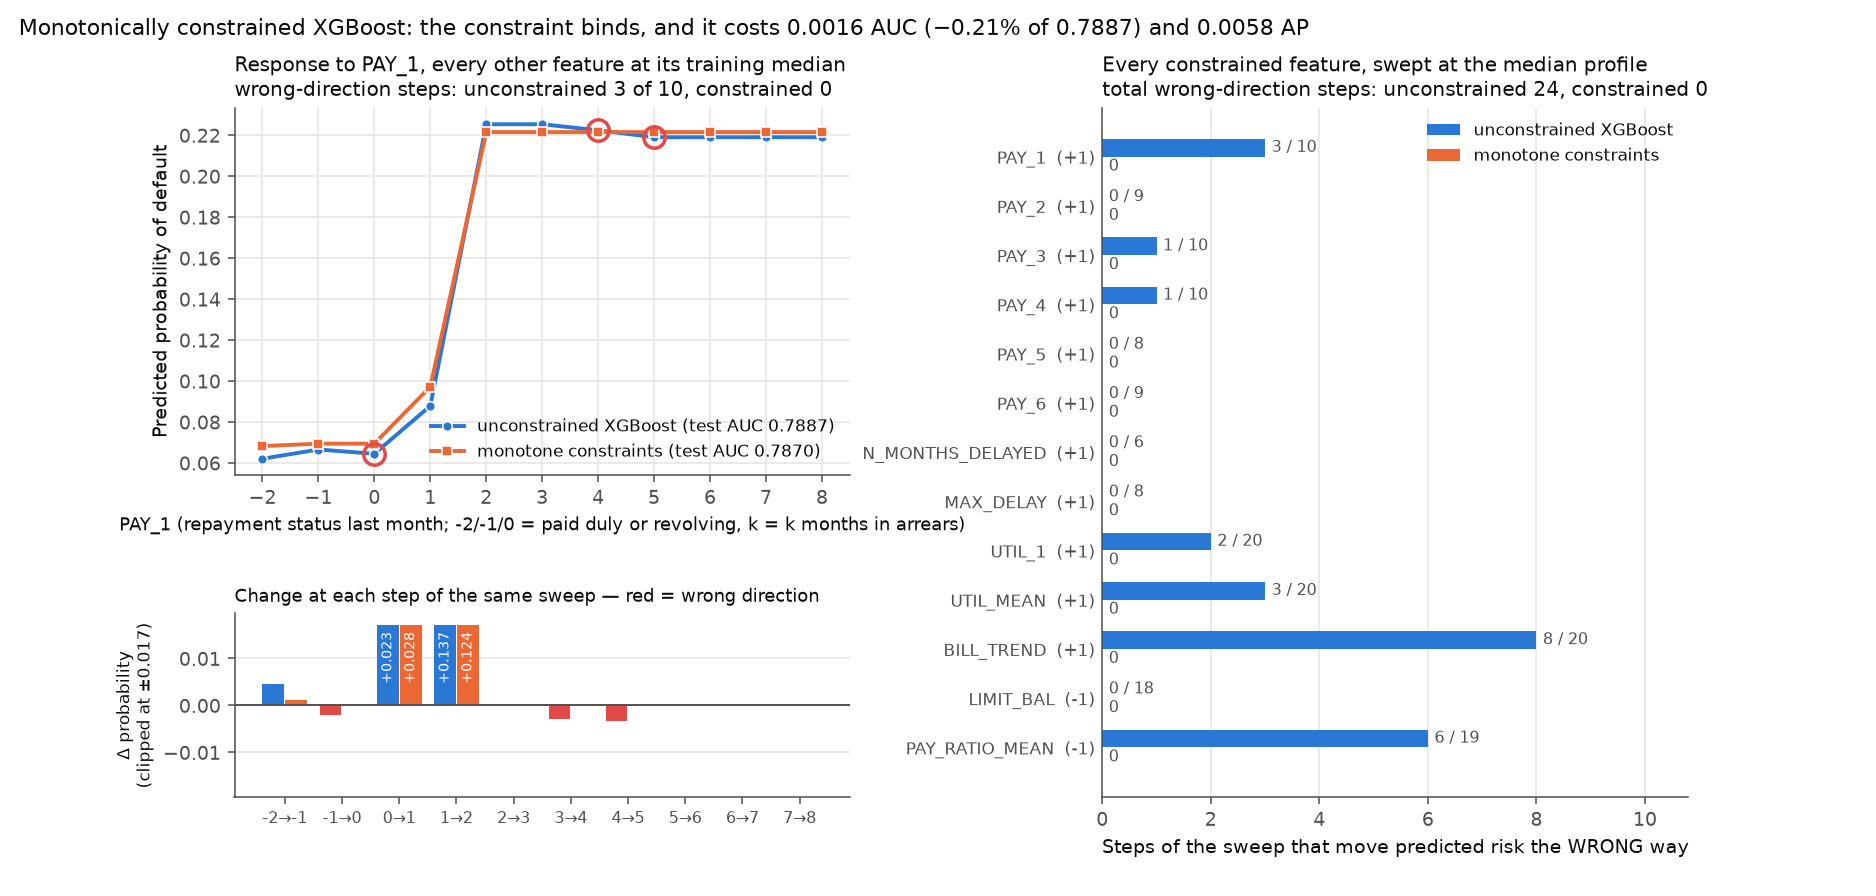
\includegraphics[width=0.92\linewidth]{monotone_pay1.png}
  \caption{Predicted probability against the most recent repayment status, with and without monotone constraints.}
  \label{fig:monotone-pay1}
\end{figure}

\begin{figure}[htbp]
  \centering
  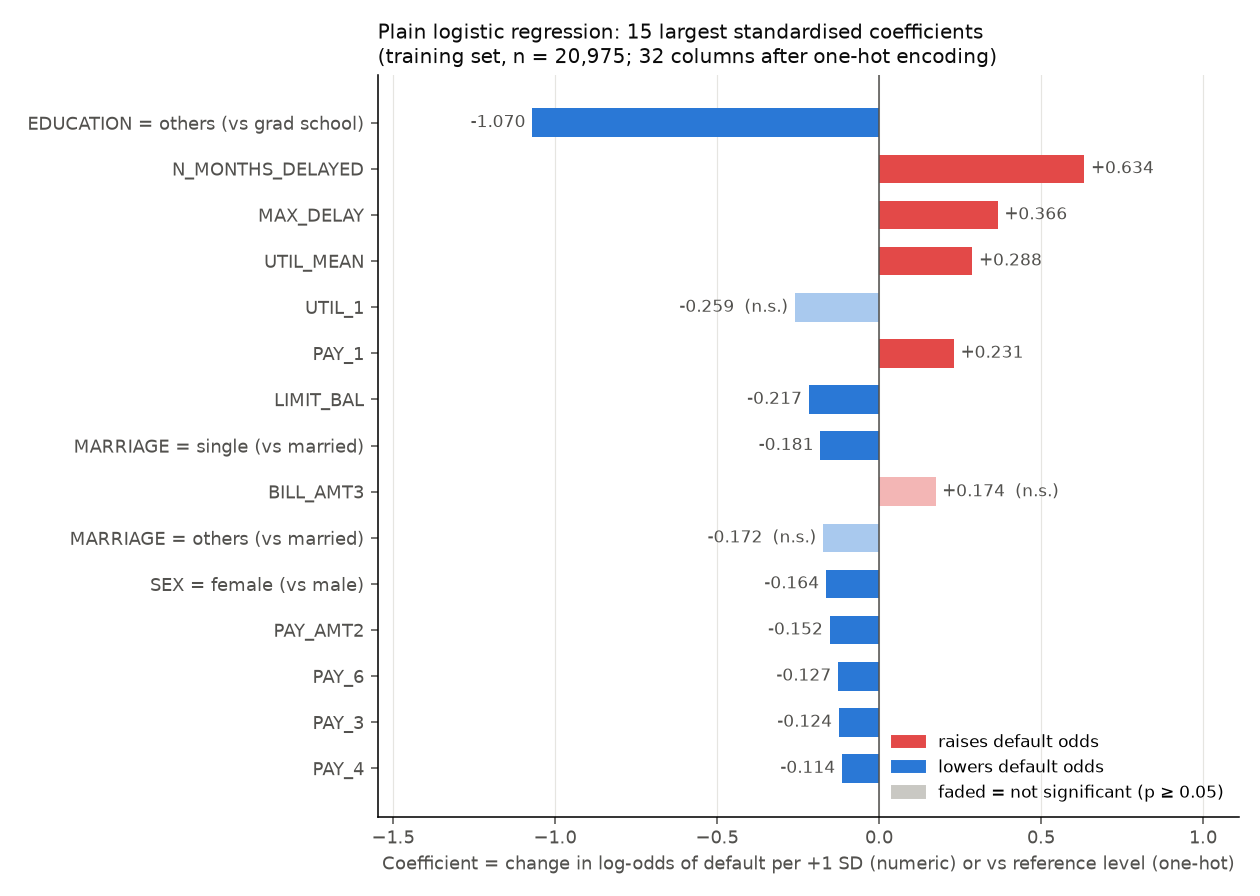
\includegraphics[width=0.92\linewidth]{logistic_coefficients.png}
  \caption{Standardised logistic coefficients.}
  \label{fig:logistic-coefficients}
\end{figure}
\clearpage

\begin{figure}[htbp]
  \centering
  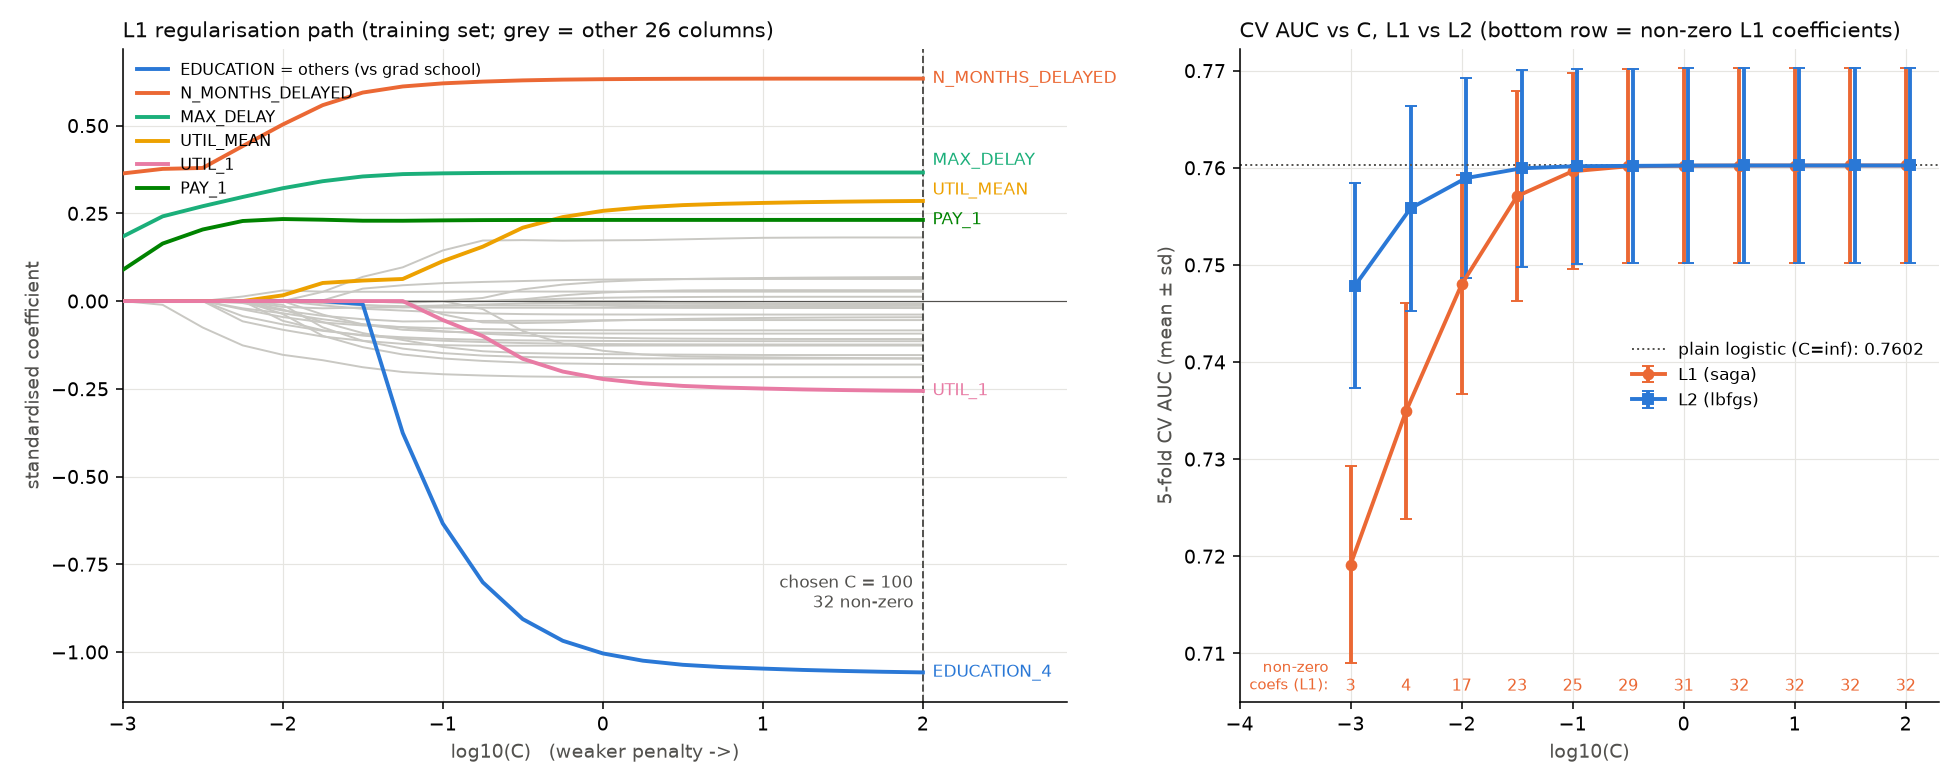
\includegraphics[width=0.92\linewidth]{logistic_l1_path.png}
  \caption{Lasso path: order of entry of the predictors as the penalty is relaxed.}
  \label{fig:logistic-l1-path}
\end{figure}

\begin{figure}[htbp]
  \centering
  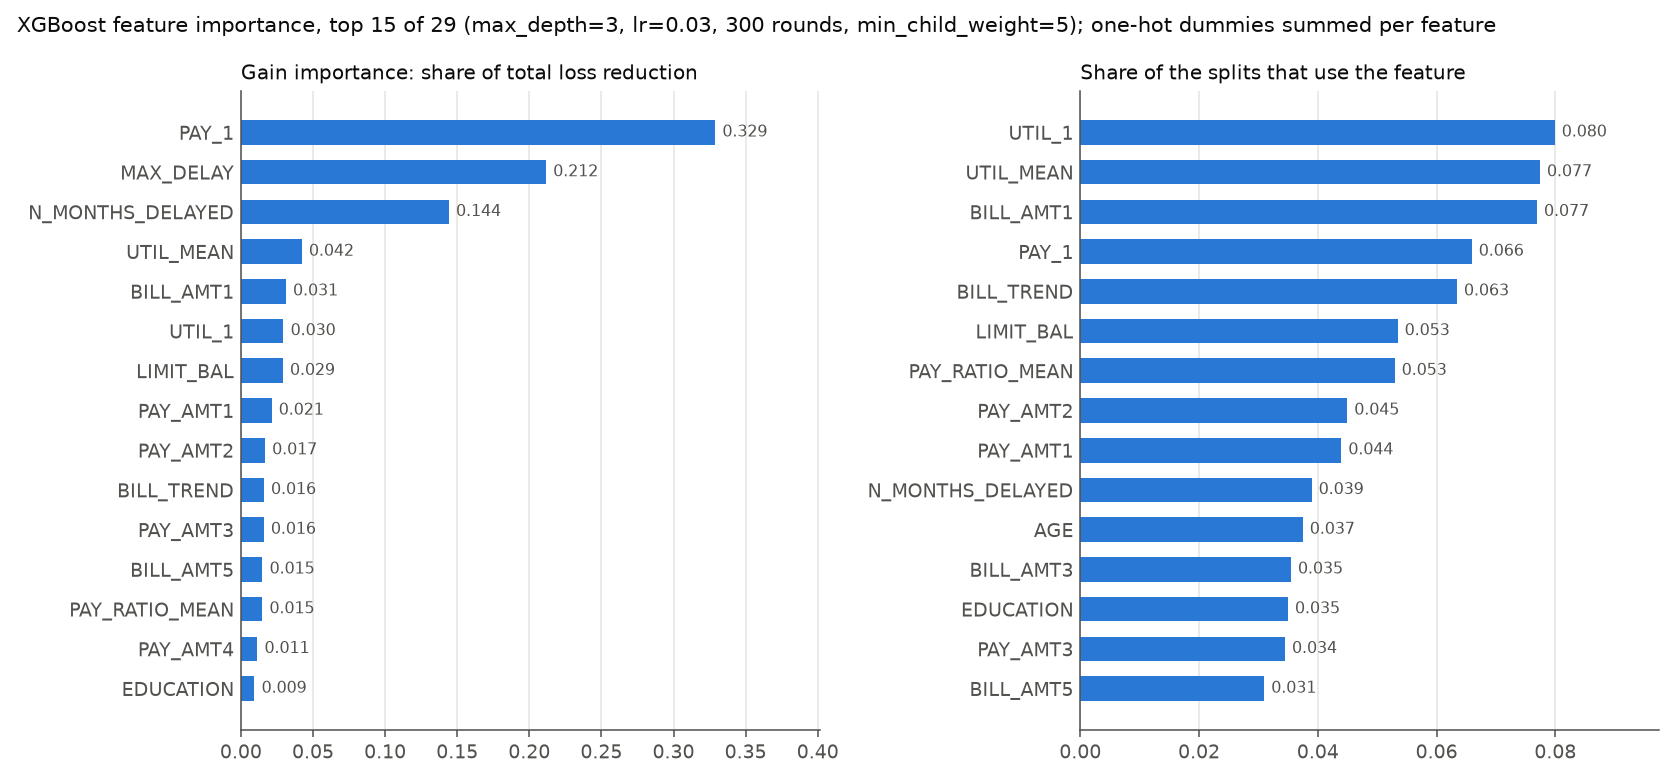
\includegraphics[width=0.92\linewidth]{xgb_importance.png}
  \caption{XGBoost gain-based importance.}
  \label{fig:xgb-importance}
\end{figure}

\begin{figure}[htbp]
  \centering
  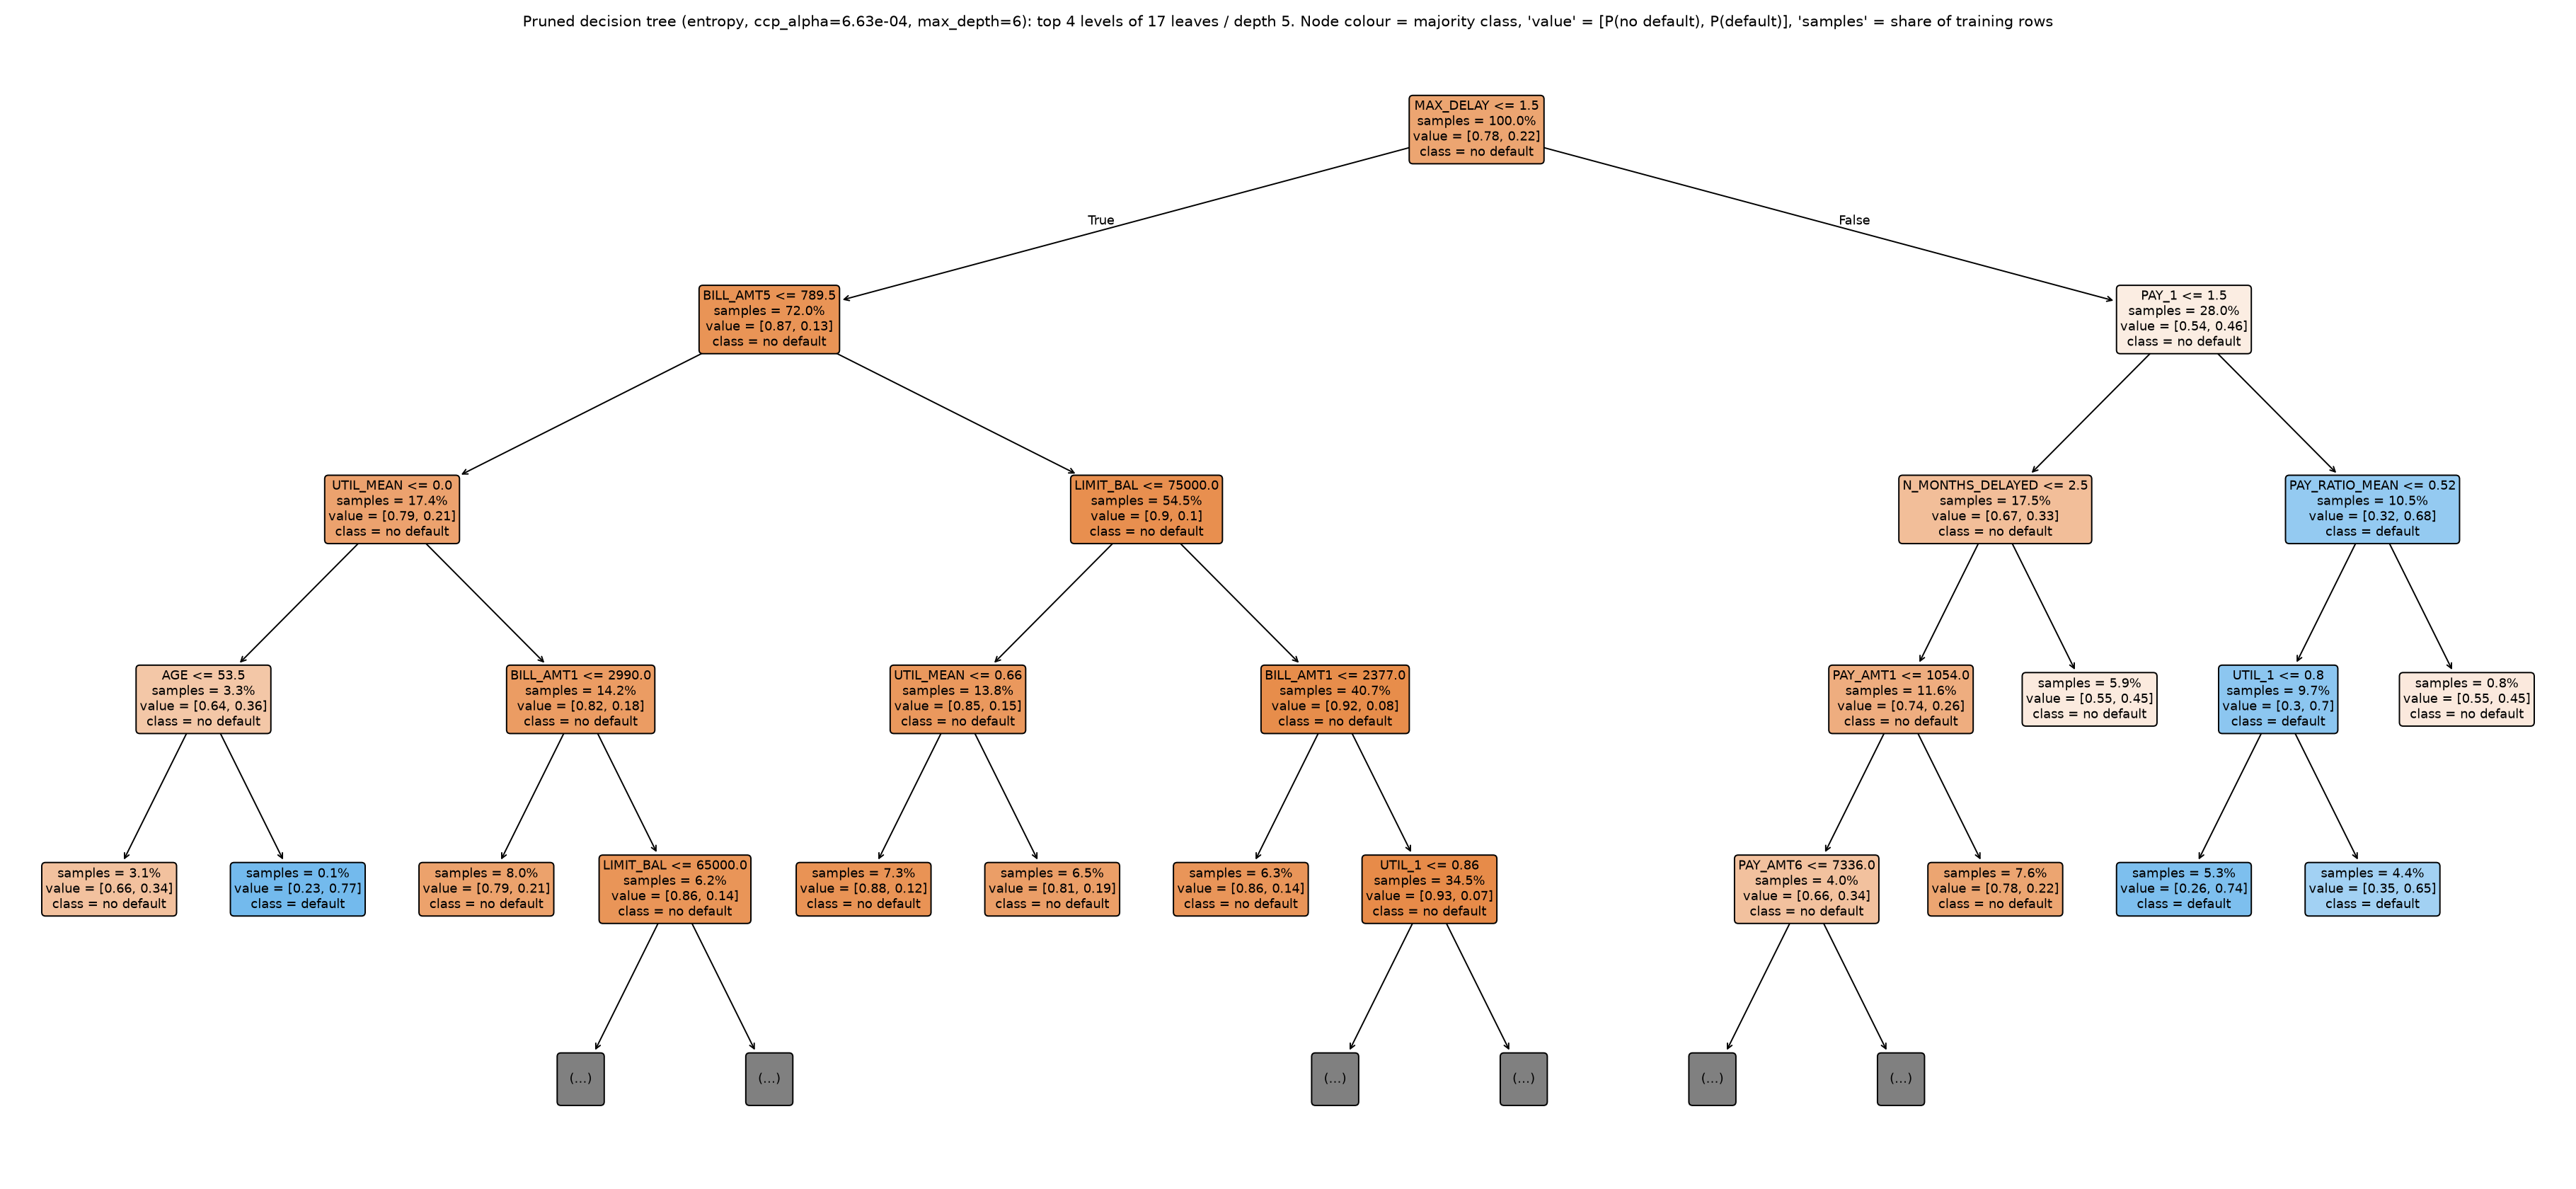
\includegraphics[width=0.92\linewidth]{tree_pruned.png}
  \caption{The pruned decision tree, top levels.}
  \label{fig:tree-pruned}
\end{figure}

\clearpage
\subsection{Class imbalance and the leakage demonstration}

\begin{figure}[htbp]
  \centering
  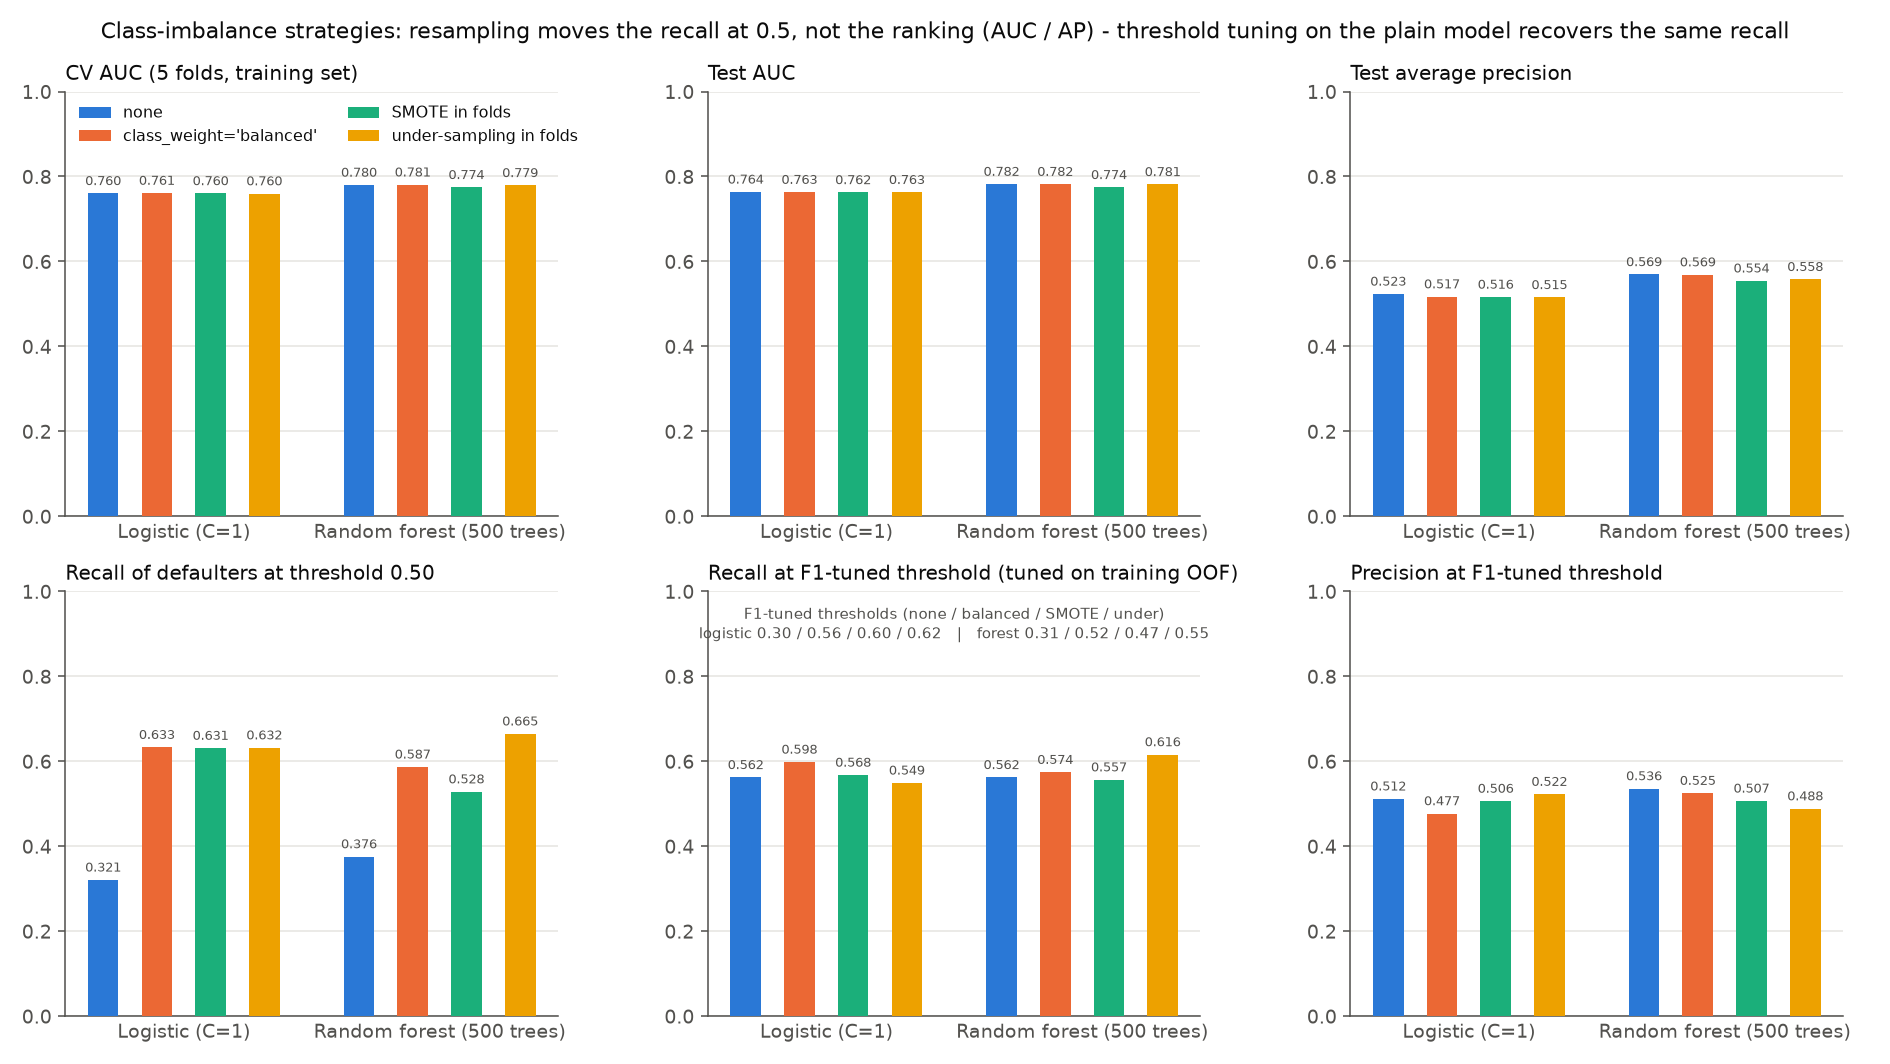
\includegraphics[width=0.92\linewidth]{imbalance_comparison.png}
  \caption{Resampling strategies applied inside the folds: AUC is unchanged, the operating point moves.}
  \label{fig:imbalance-comparison}
\end{figure}

\begin{figure}[htbp]
  \centering
  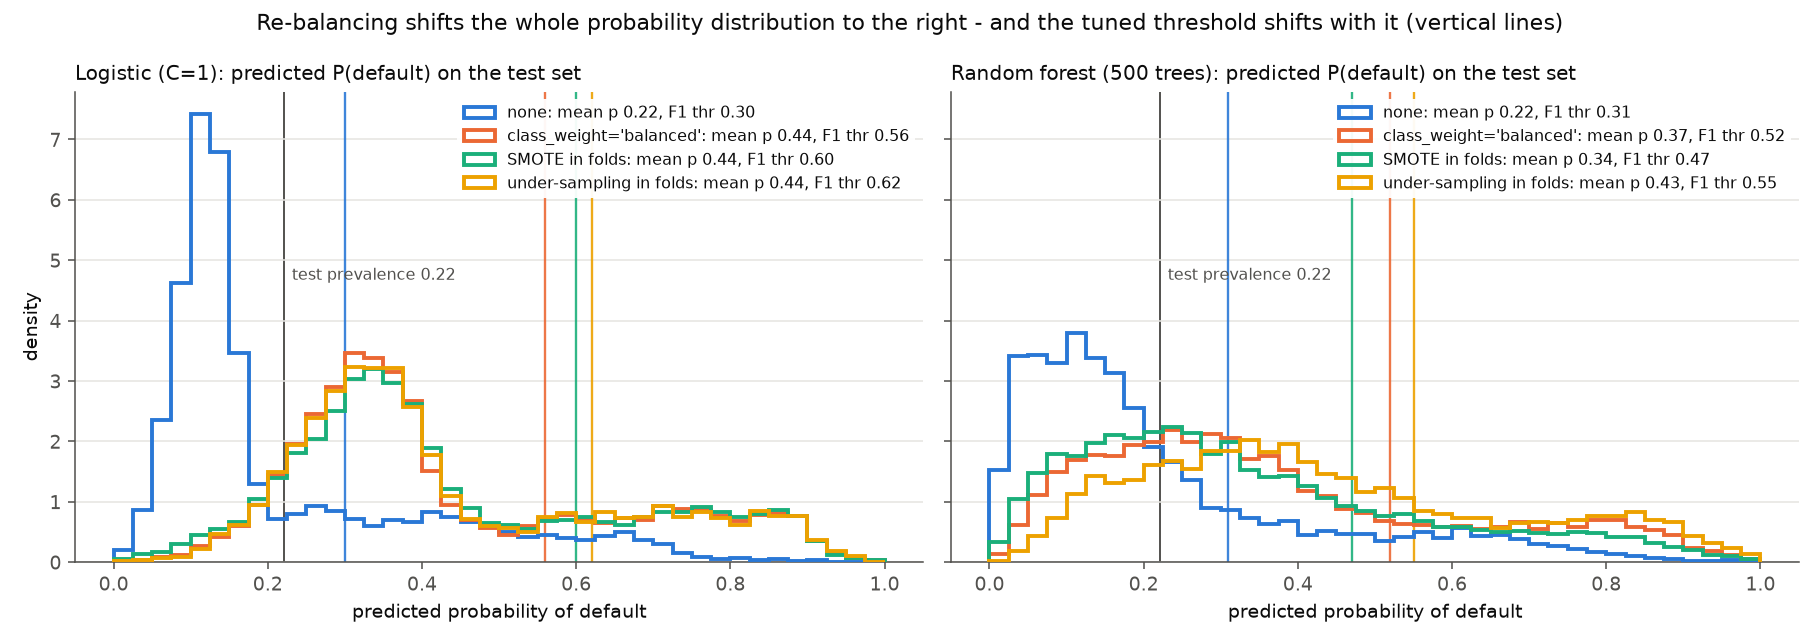
\includegraphics[width=0.92\linewidth]{imbalance_threshold_shift.png}
  \caption{Where each resampling strategy puts the tuned threshold.}
  \label{fig:imbalance-threshold-shift}
\end{figure}

\begin{figure}[htbp]
  \centering
  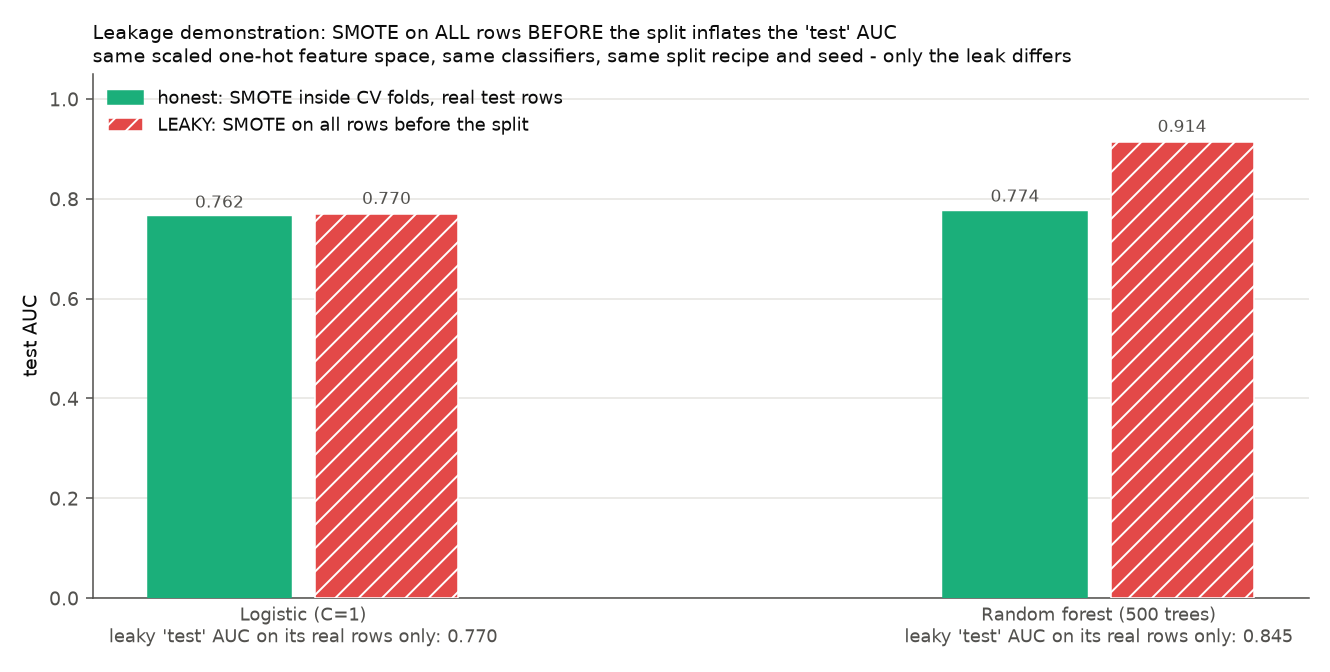
\includegraphics[width=0.92\linewidth]{imbalance_leakage_demo.png}
  \caption{Negative control: SMOTE applied before the split inflates the apparent test AUC.}
  \label{fig:imbalance-leakage-demo}
\end{figure}
\clearpage

\clearpage
\subsection{Model selection diagnostics}

\begin{figure}[htbp]
  \centering
  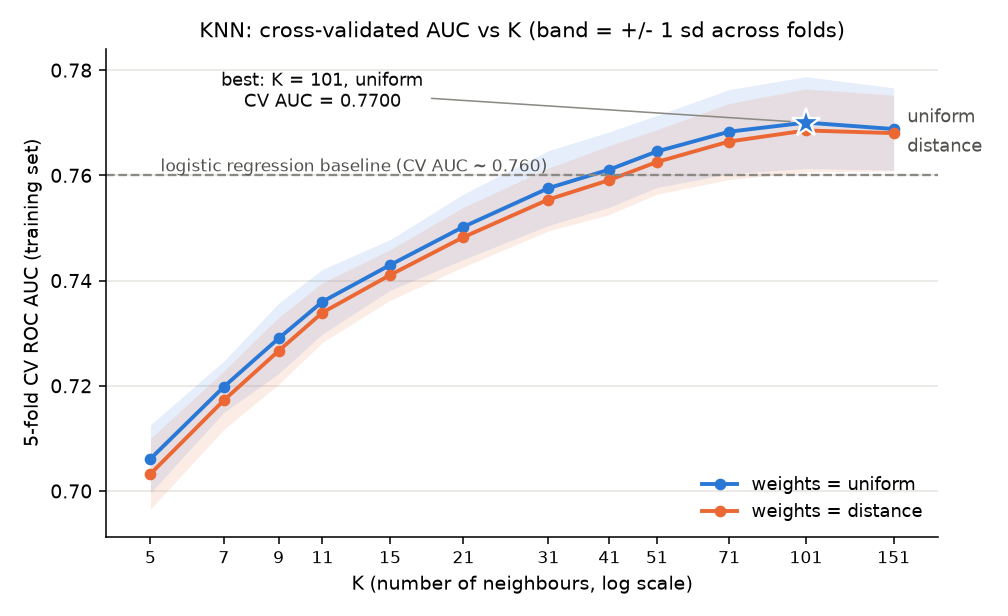
\includegraphics[width=0.92\linewidth]{knn_cv_auc_vs_k.png}
  \caption{KNN: cross-validated AUC against $K$.}
  \label{fig:knn-cv-auc-vs-k}
\end{figure}

\begin{figure}[htbp]
  \centering
  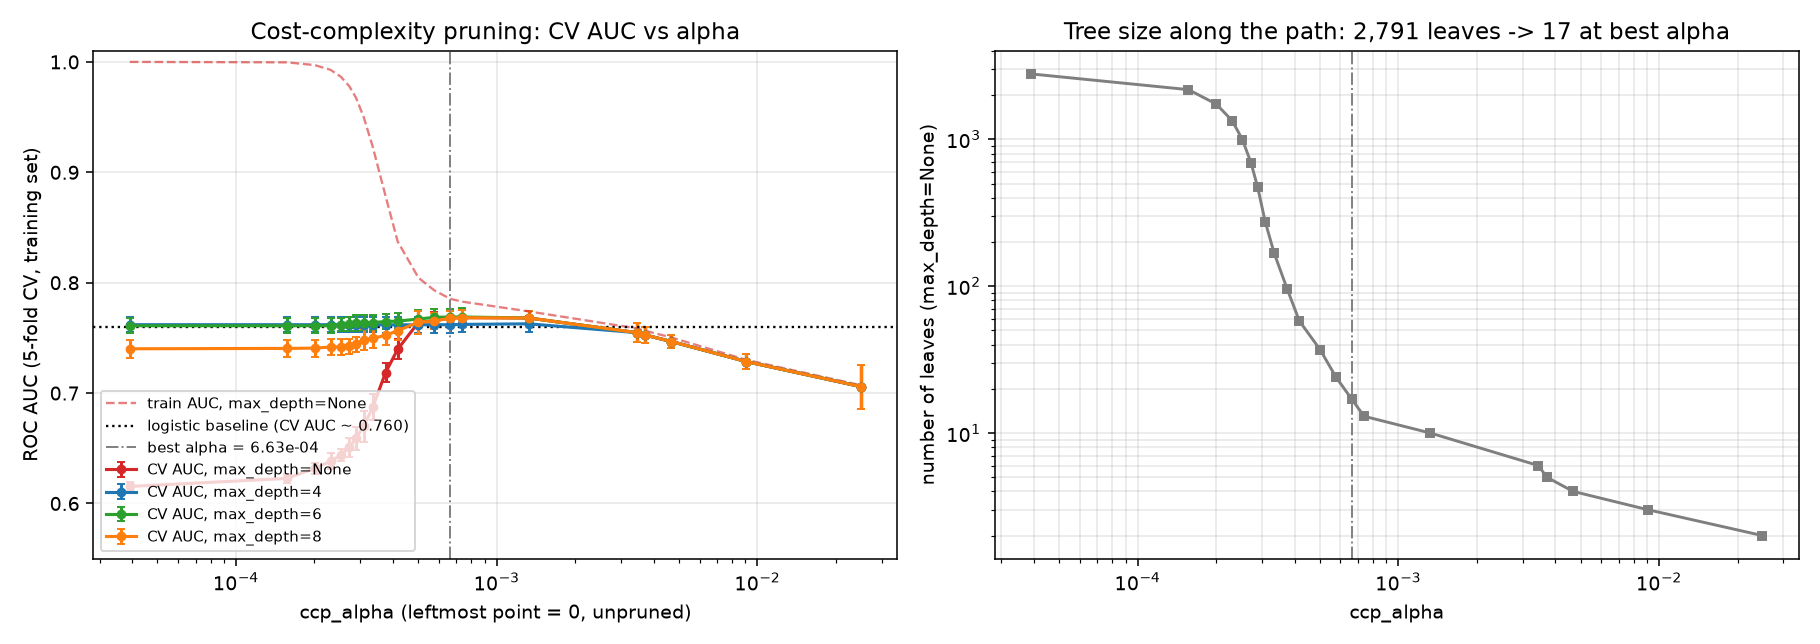
\includegraphics[width=0.92\linewidth]{tree_cv_auc_vs_alpha.png}
  \caption{Cost-complexity pruning path.}
  \label{fig:tree-cv-auc-vs-alpha}
\end{figure}

\begin{figure}[htbp]
  \centering
  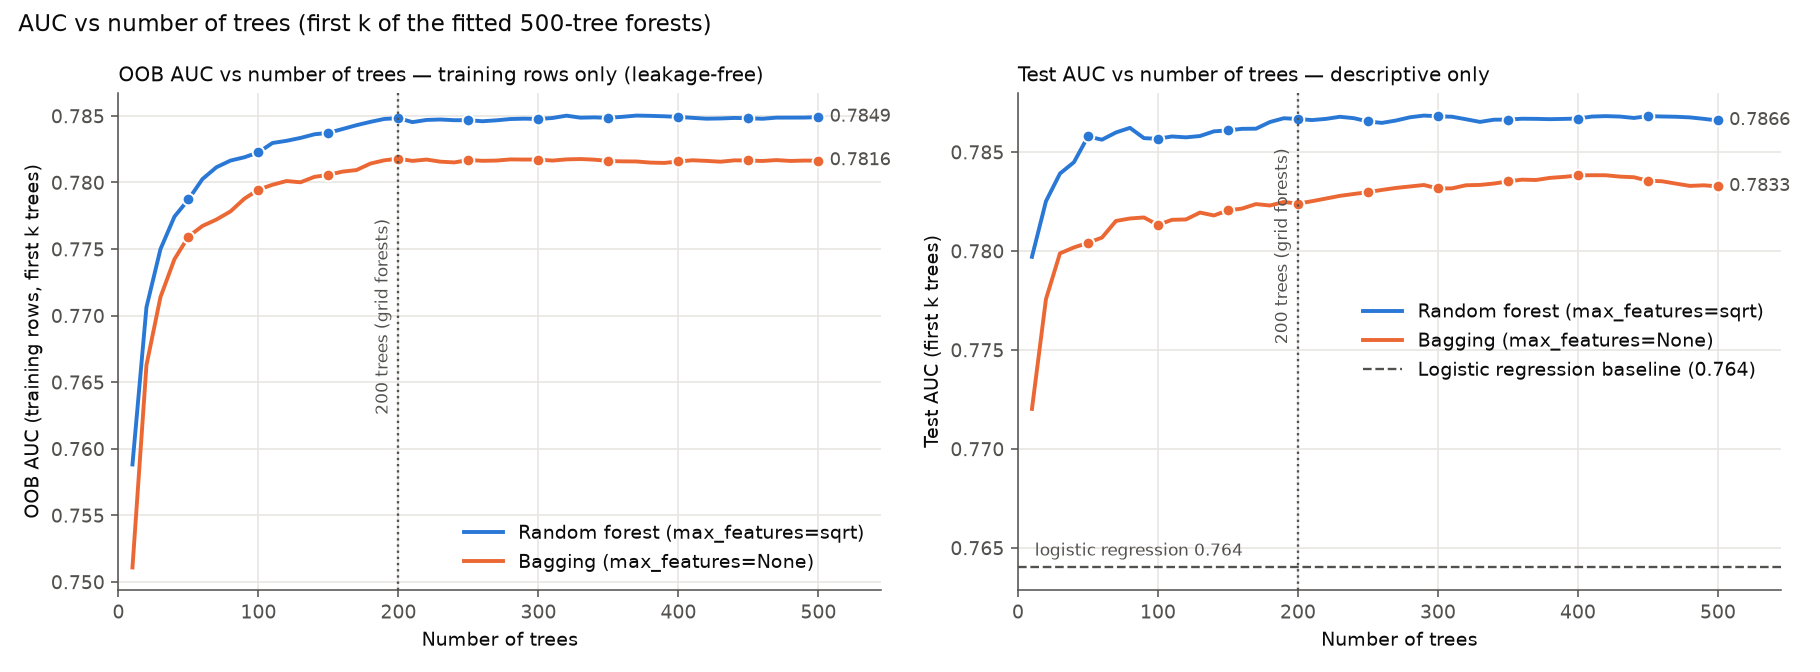
\includegraphics[width=0.92\linewidth]{rf_auc_vs_ntrees.png}
  \caption{Random forest: out-of-bag and test AUC against the number of trees.}
  \label{fig:rf-auc-vs-ntrees}
\end{figure}

\begin{figure}[htbp]
  \centering
  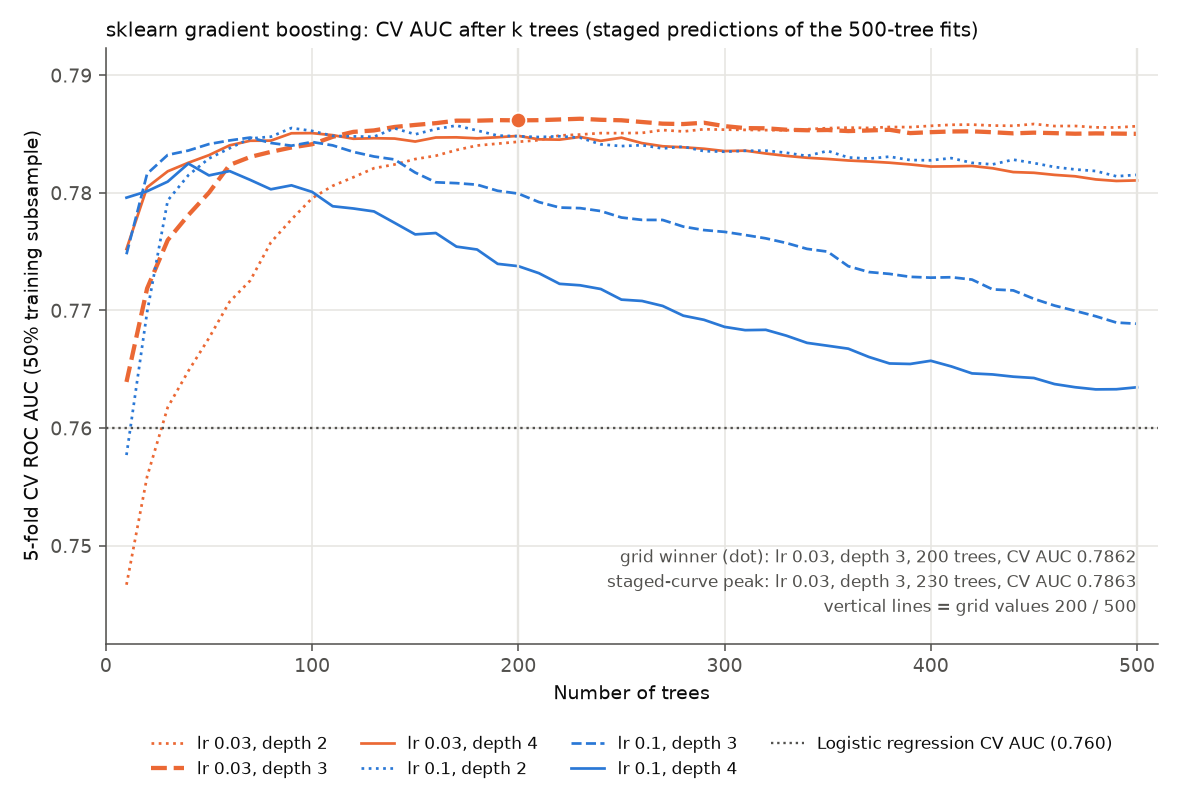
\includegraphics[width=0.92\linewidth]{gbm_learning_curve.png}
  \caption{Gradient boosting: cross-validated AUC against the number of rounds.}
  \label{fig:gbm-learning-curve}
\end{figure}

\begin{figure}[htbp]
  \centering
  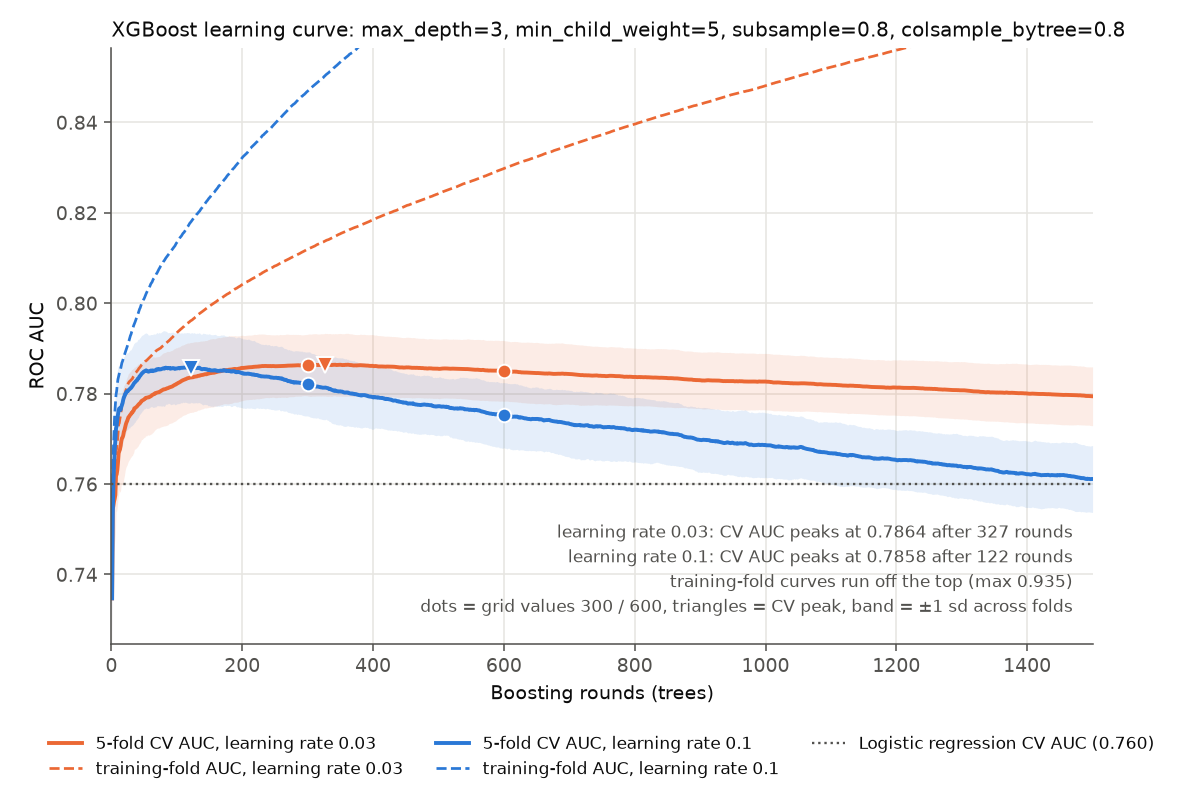
\includegraphics[width=0.92\linewidth]{xgb_learning_curve.png}
  \caption{XGBoost learning curves at two learning rates.}
  \label{fig:xgb-learning-curve}
\end{figure}

\begin{figure}[htbp]
  \centering
  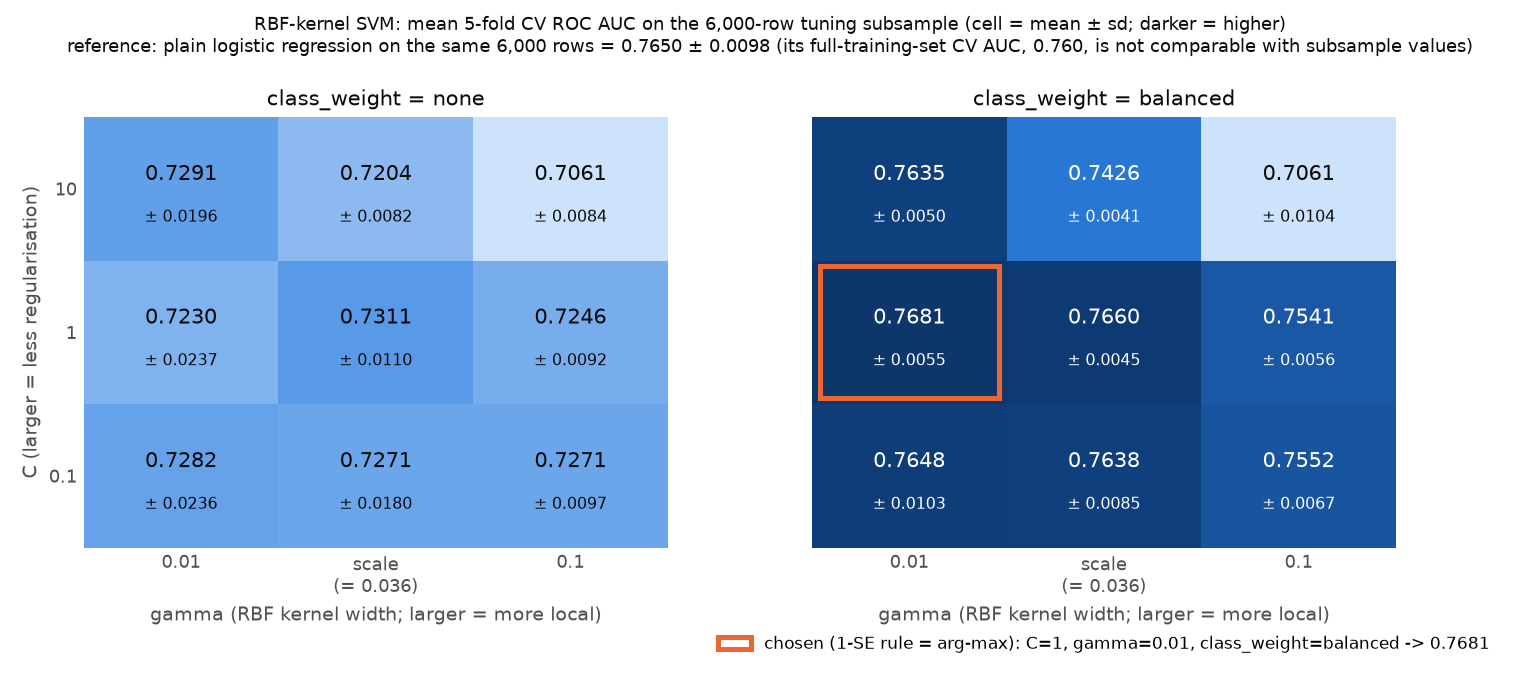
\includegraphics[width=0.92\linewidth]{svm_rbf_cv_heatmap.png}
  \caption{RBF support-vector machine: cross-validated AUC over $C$ and $\gamma$.}
  \label{fig:svm-rbf-cv-heatmap}
\end{figure}
\clearpage

\begin{figure}[htbp]
  \centering
  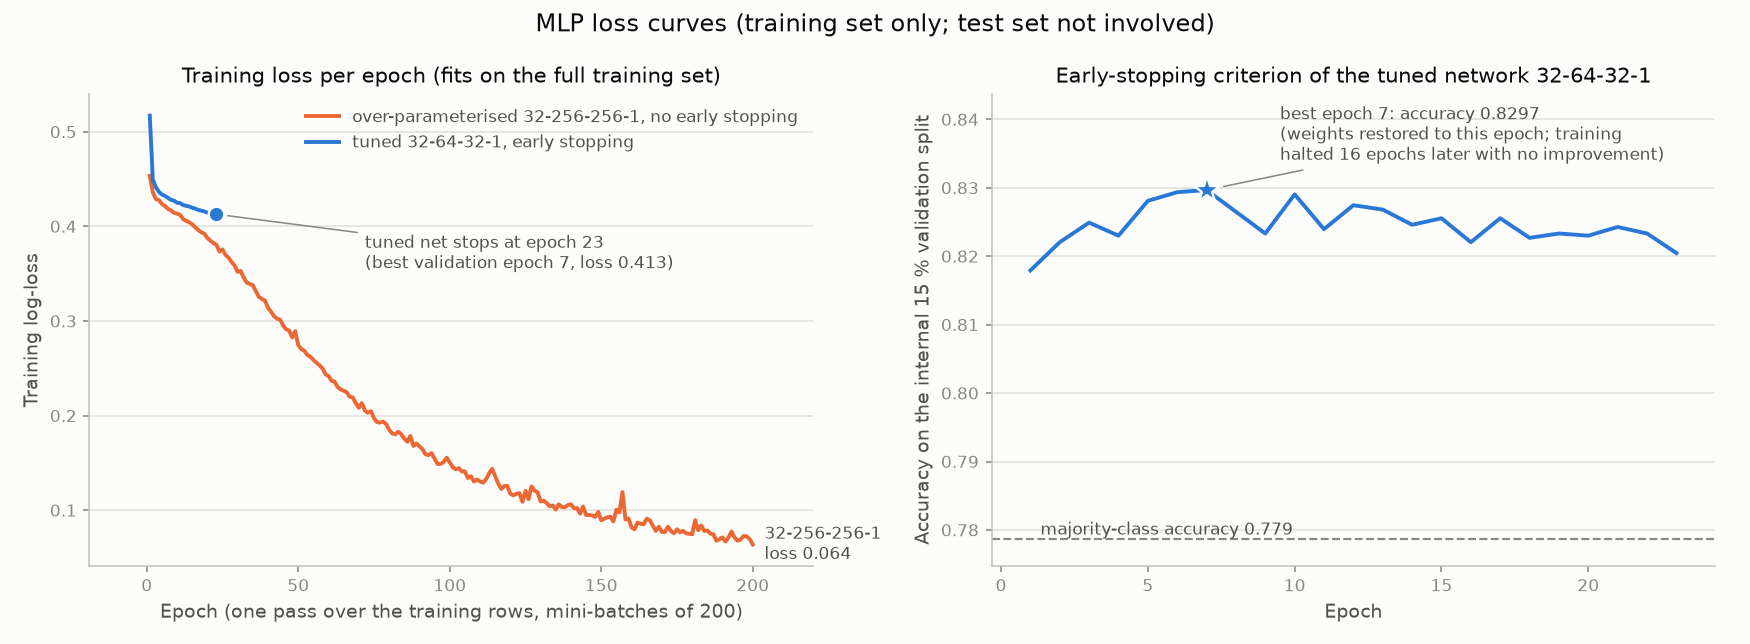
\includegraphics[width=0.92\linewidth]{mlp_loss_curve.png}
  \caption{Neural network: training loss and validation AUC by epoch.}
  \label{fig:mlp-loss-curve}
\end{figure}

\begin{figure}[htbp]
  \centering
  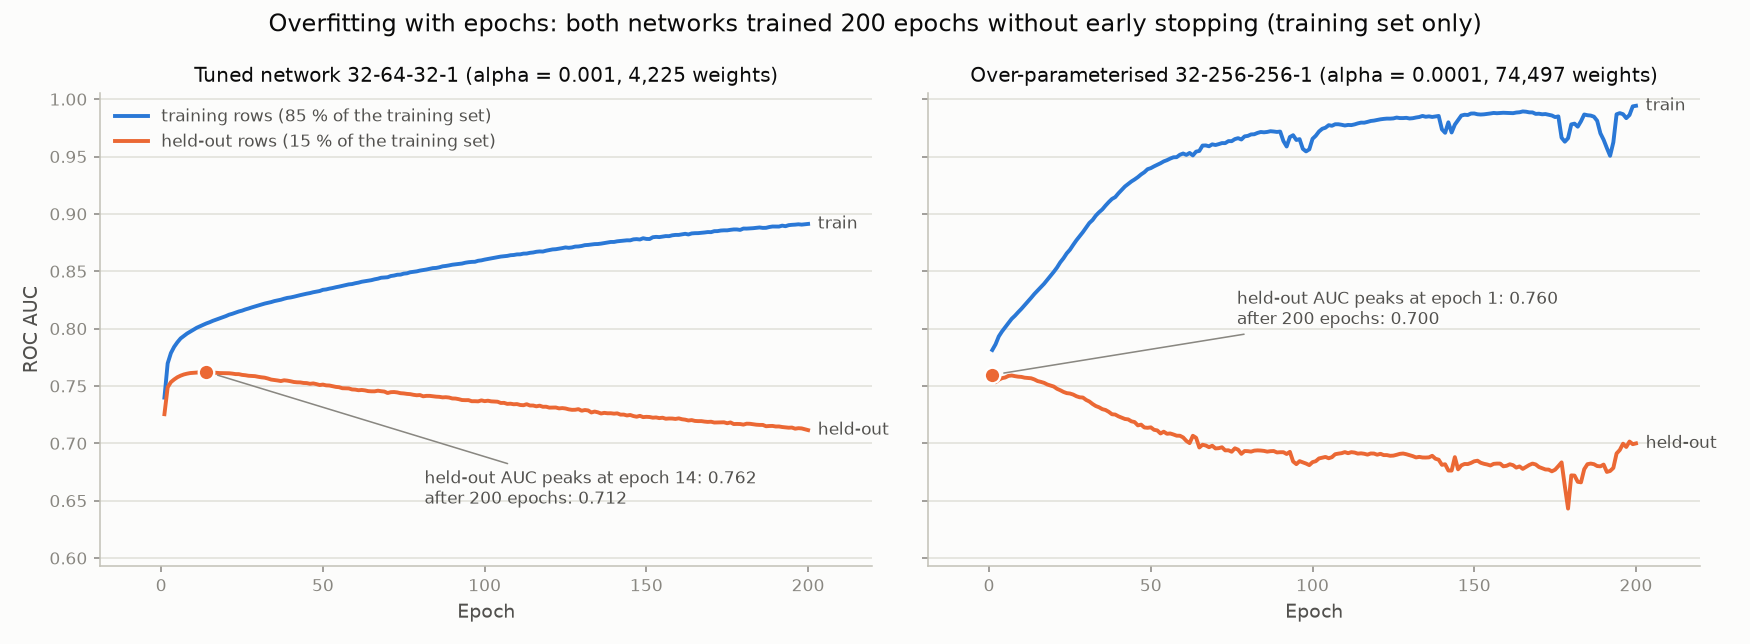
\includegraphics[width=0.92\linewidth]{mlp_overfit_epochs.png}
  \caption{Over-parameterised network: the over-fitting diagnostic.}
  \label{fig:mlp-overfit-epochs}
\end{figure}

\begin{figure}[htbp]
  \centering
  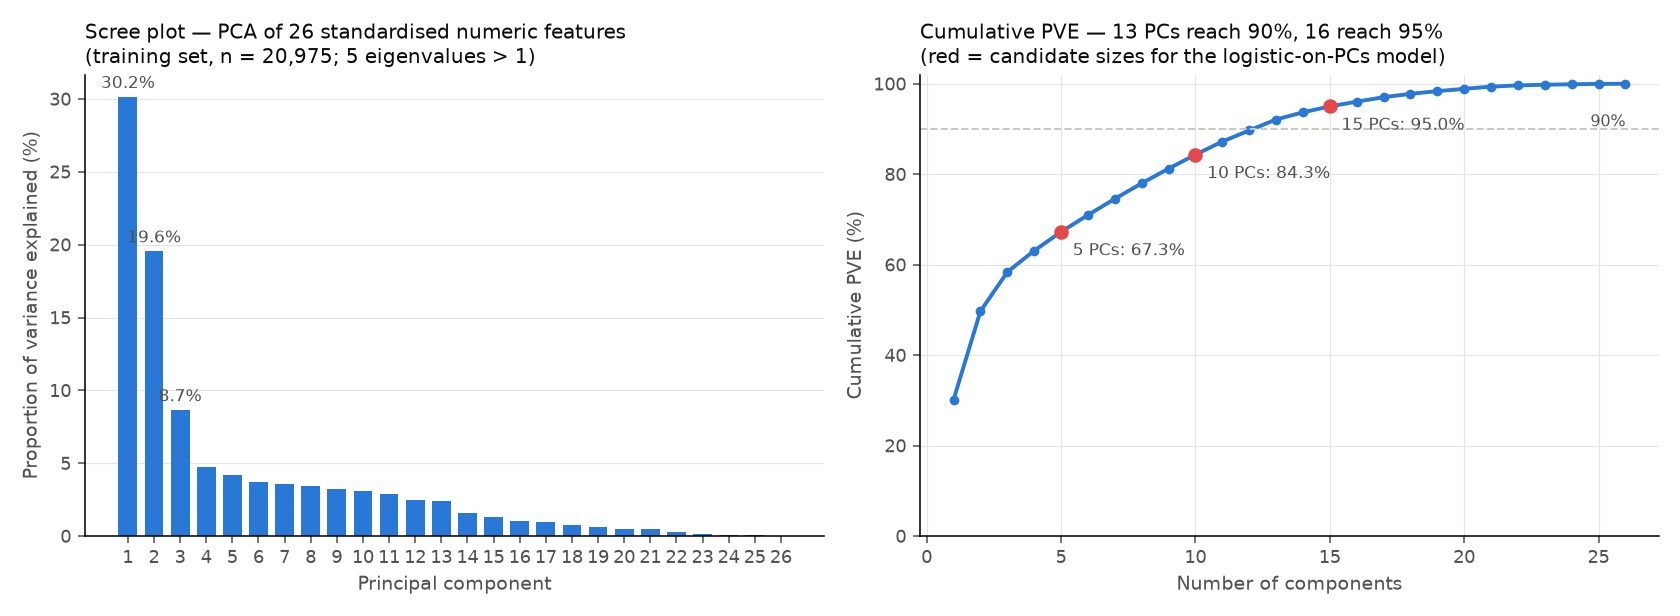
\includegraphics[width=0.92\linewidth]{pca_scree.png}
  \caption{PCA scree plot and cumulative variance explained.}
  \label{fig:pca-scree}
\end{figure}

\begin{figure}[p]
  \centering
  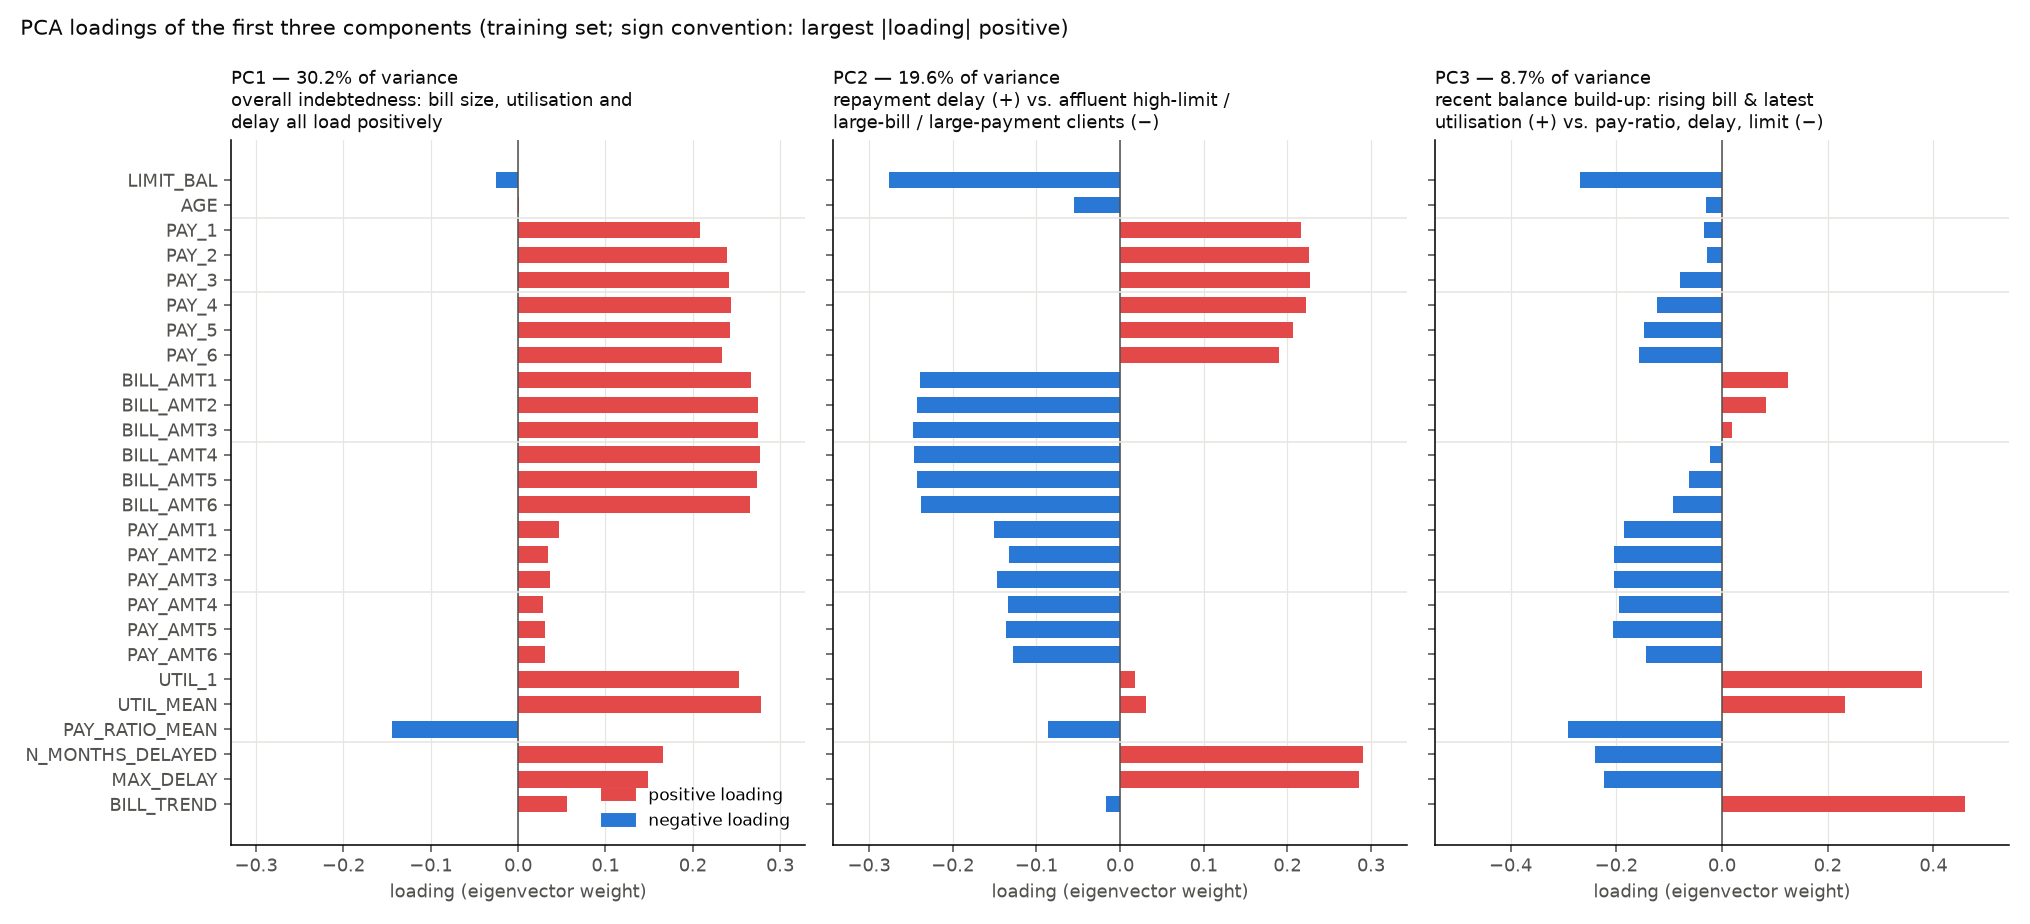
\includegraphics[width=1.0\linewidth]{pca_loadings.png}
  \caption{Loadings of the first three principal components.}
  \label{fig:pca-loadings}
\end{figure}

\begin{figure}[htbp]
  \centering
  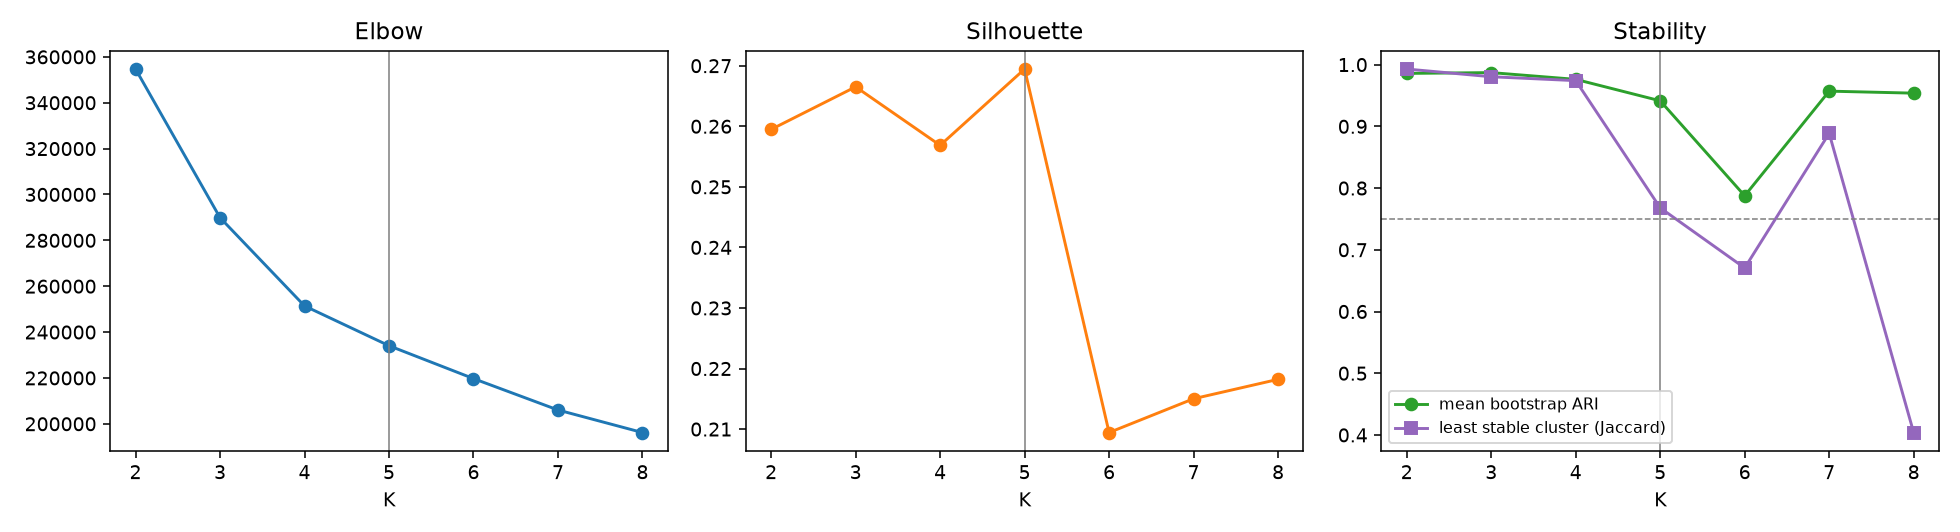
\includegraphics[width=0.92\linewidth]{kmeans_selection_repro.png}
  \caption{K-means on the first 10 principal components: silhouette, bootstrap ARI and minimum cluster Jaccard against $K$ (Table~\ref{tab:a-kselect}); reproduction on 21 October of RUAN Hangjing's 30 September analysis, training partition only.}
  \label{fig:kmeans-selection-repro}
\end{figure}



\end{document}
